\chapter[Hadron production in pion-carbon interactions]{Hadron production in pion-carbon interactions}
\label{sec:hadron}

\note{Introduction}

\note{Make it clear what was previously done}

%%%%%%%%%%%%%%%%%%%%%%%%%%%%%%%%%%%%%%%%
\section{Dataset and simulations}
\label{sec:hadron:data}

\note{DONE}

The $\pi^-$-C data were collected by \NASixtyOne in 2009 at two beam energies:
158 and 350 \GeVc. The $\pi^-$ beam was a secondary one
produced by the collisions of a 400 \GeVc proton beam against
a 10 cm long beryllium target. The carbon target consisted of
an isotropic graphite plate with 2 cm thickness along the beam axis.
For more details about the $\pi^-$-C dataset see Ref.\cite{\RhoPaper}.

Two trigger modes are relevant for the present analysis: the beam and
interaction trigger, which are denominated by T1 and T2 respectively.
The definition of T1 is
$\text{S1}\wedge\text{S2}\wedge\overline{\text{V0}}\wedge\overline{\text{V1}}\wedge\overline{\text{V1}'}$
and T2 is
$\text{T1}\wedge\overline{\text{S4}}$.
While the T1 assures that a beam particle
reached the target position,
the T2 is suppose to eliminate events in which a beam particle
crossed the target without interacting. Because of the position of
the S4 detector, it can also be reached 
by high energy particles produced by the inelastic interaction at the target,
causing the removal of events which are desirable for the analysis.
It was verified that the rate of this events is very small and they do not
produce a significant bias on our results.
For more details about the trigger modes see Ref.~\cite{MartinThesis}.
The standard calibration algorithm applied to \NASixtyOne
data is described in Ref.~\cite{Abgrall:2008zz}.

To estimate and remove from the particle spectra the contribution
of interactions that do not occur at the target, a set of data
were also taken with the target removed. The amount of target
removed data is approximately 10\% of the total data taken.
In~\cref{sec:hadron:spec} we describe 
the procedure for the target removed subtraction.

The Monte Carlo simulation sets were generated by first generating
the primary interactions using hadronic interaction models and
then by passing the produced particles through a detailed
detector simulation based on \GeantThree package~\cite{Brun:1994aa}.
Three hadronic interaction models were used: \EposLong~\cite{\EposPaper},
\DPMJetLong~\cite{\DPMJetPaper} and \QGSJetLong~\cite{\QGSJetPaper}.
For each beam energy and hadronic interaction model,
a simulation set was produced with approximately the same event
number as the datasets. 
Both the data and the simulations were reconstructed by the standard
\NASixtyOne reconstruction chain~\cite{Abgrall:2011ae}. 

%%%%%%%%%%%%%%%%%%%%%%%%%%%%%%%%%%%%%%%%
\section{Event selection}
\label{sec:hadron:event}

\note{DONE}

The first step of the event selection is the upstream cuts,
which are based on the information from the beam detectors.  
The upstream cuts are:
\begin{enumerate}[label=(\roman*)]
\item CEDAR cut  to identify the beam particle type and then remove
  the contributions from non-pion particles.
\item WFA cut  that uses the time information from the S1 detector
  to exclude events in which a second beam particle was detected
  with a time difference shorter than 2 $\mu$s.
\item BPD cut that uses the information from the three BPD detectors
  to assure a good quality measurements of the beam position at the
  target plan. These measurements are important to constraint the
  main vertex position during the event reconstruction.
\end{enumerate}
More details about the upstream cuts can be found in Ref.~\cite{MartinThesis}.
\note{more refs}
Since the beam detectors are not implemented in the simulations,
the upstream cuts are applied only to the data.

The second step is the event cuts, which are applied both to data
and simulations. The three event cuts are:
\begin{enumerate}[label=(\roman*)]
\item Trigger cut  that selects events which are
  defined as T2 trigger type (see~\cref{sec:hadron:data}
  for the trigger definitions).
\item Main vertex cut to remove events in which the main vertex
  is not fitted during the event reconstruction.
\item Vertex Z cut  to remove events in which the z coordinate of the fitted
  main vertex is farer than 17 cm from the main vertex position measured
  by the BPD detectors. This cut is meant to reduce the contribution from
  out-of-target interactions. 
\end{enumerate}
In~\cref{tab:hadron:stat} we show the number of available events
after the event selection for the data and simulation sets.

\warning{include target removed in the table}

\begin{table}
  \begin{center}
    \begin{tabular}{|l|c|c|} \hline
                  & 158 GeV/c       & 350 GeV/c \\ \hline
      Data        & 3.46 $10^6$     & 3.04 $10^6$ \\
      \EposLong   & 3.71 $10^6$     & 3.12 $10^6$ \\
      \DPMJetLong & 3.92 $10^6$     & 3.47 $10^6$ \\
      \QGSJetLong & 3.71 $10^6$     & 3.06 $10^6$ \\ \hline
    \end{tabular}
    \caption{}
    \label{tab:hadron:stat}
  \end{center}
\end{table}

%%%%%%%%%%%%%%%%%%%%%%%%%%%%%%%%%%%%%%%%
\section{Track selection}
\label{sec:hadron:trackselection}

\note{DONE}

\note{define labels identified spectra and \vzero analysis}

The following selection criteria were applied to the measured tracks
for the identified spectra analysis:
\begin{enumerate}[label=(\roman*)]
\item The reconstructed track must be contained in the detector acceptance,
  that is basically defined as regions in ($\phi$,\pp,\pT) phase space
  in which the selection efficiency is larger than 90\%. A second effect
  that is also accounted in the definition of the acceptance is the tracks that
  hit directly the S4 detector and are not removed by the T2 trigger selection.
  While the selection efficiency contribution is estimated with Monte Carlo simulation,
  the directly hits on S4 are removed based on the measured tracks.
  The full description of the acceptance selection can be found in Ref.\cite{MartinThesis}.
\item The total number of clusters on the track must be greater than or equal to 25.
\item The sum of clusters on both VTPCs must be greater than or equal to 12, or
  the number of cluster on the GTPC must be greater than of equal to 6.
\item The distance between the extrapolated track to the interaction plane and the
  interaction point, that is called impact parameter, must be smaller than 4 cm
  in the both horizontal and vertical plane.
\end{enumerate}
\note{some explanations on the idea of the acceptance cut}
More details about the track selection
can be found in Ref.~\cite{MartinThesis}.

\warning{paragraph with RST and WST definitions}


%%%%%%%%%%%%%%%%%%%%%%%%%%%%%%%%%%%%%%%%
\section{\vzero selection}
\label{sec:hadron:vzeroselection}

\note{DONE}

The \vzero selection criteria used for the \vzero analysis
is the following:
\begin{enumerate}[label=(\roman*)]
\item The selected vertex must be identified as a \vzero type vertex.
\item The number of daughter tracks of the vertex must be equal to 2.
\item Both daughter tracks must be of opposite charges.
\item The total number of cluster has to be greater than 30 for both tracks
\item At least one track has to have more than 15 clusters in the VTPCs
\end{enumerate}
These selection criteria are standard ones in \NASixtyOne analysis.
Further cuts on the \vzeros will be applied at the signal extraction
step (see~\cref{sec:hadron:signal:cuts}).

Since it is not possible to define the detector acceptance for
the \vzeros analogously to what is done for the tracks, the possible
discrepancies between data and simulations on the borders of the acceptance
will be accounted on the systematic uncertainties (see~\cref{sec:hadron:spec:syst}).
Because these tracks on the borders have small number of clusters,
the systematic uncertainty will be estimated by changing the minimum number
of clusters on both tracks from 30 to 20. 


%%%%%%%%%%%%%%%%%%%%%%%%%%%%%%%%%%%%%%%%
\section{Phase space binning}

\note{DONE}

Both identified spectra and \vzero analysis were done
by splitting the data in bins in a 2-dimensional
phase space of the \pp and \pT variables. For the
identified spectra analysis only one phase space
binning configuration is defined. The intervals in \pp
are nearly uniform in $\log p$, with small adjustments in a way
that moves the crossing points of the energy deposit function
of different particles closer to the center of the bins.
Since some of these bins in the crossing regions
will be removed from the analysis (see~\cref{sec:hadron:dedx:sde}),
this strategy has shown effective to reduce the number of
removed bins. The average width of the \pp intervals is
$\Delta\log\pp=0.1$. Concerning the \pT intervals, the bin width
increases with \pT, being the width of the shorter and the longer one
$\Delta \pT=0.1$ and  $\Delta\pT=0.5$, respectively.  
In~\cref{fig:hadron:binning:dedx} we show the binning configuration
for the identified spectra analysis.


%%%%%%%%%%%%%% BINNING DEDX %%%%%%%%%%%%%%%
\begin{figure}[!ht]
  \centering
  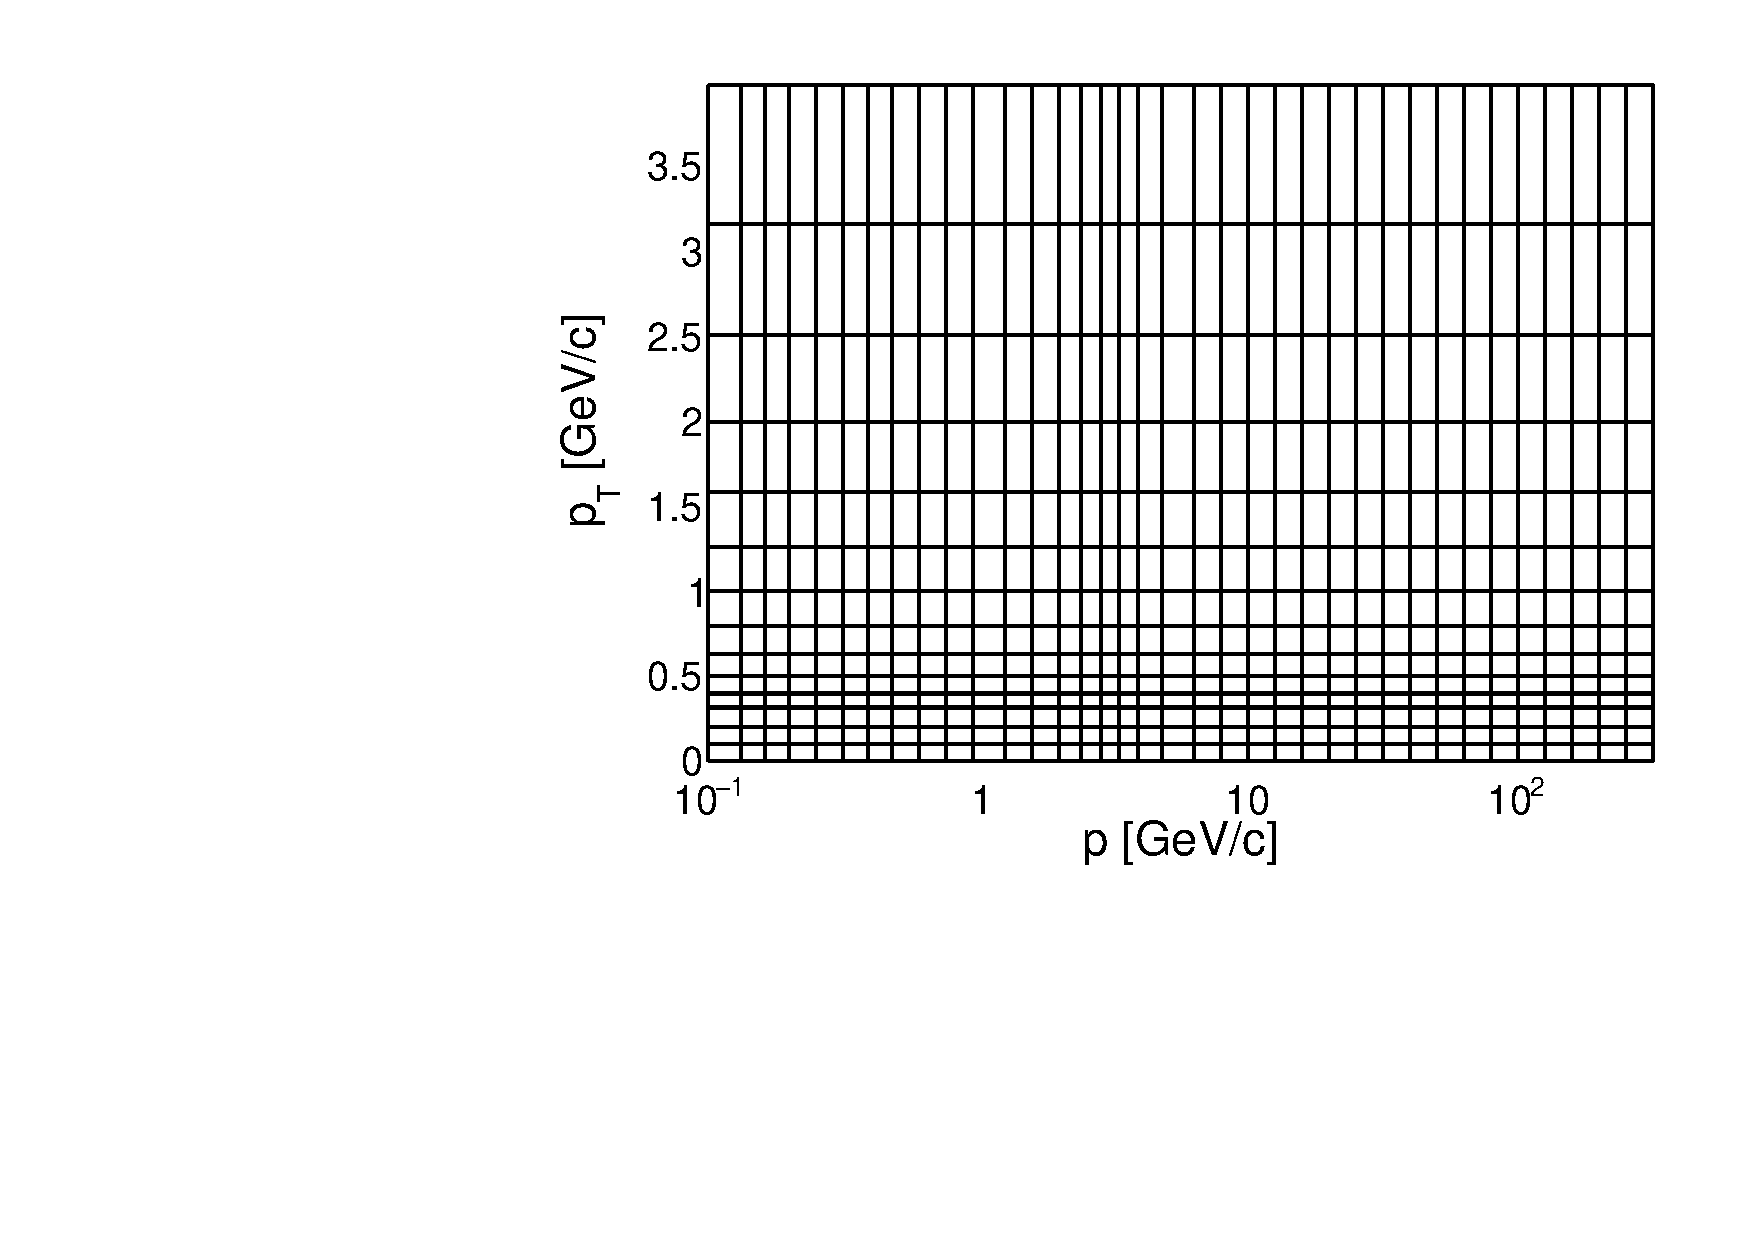
\includegraphics[clip, rviewport=0 0 1 1,width=0.5\textwidth]{DedxBinning}
  \caption{}
  \label{fig:hadron:binning:dedx}
\end{figure}

Since the \vzero analysis is done independently for the three target particles,
the phase space binning is not required to be unique. Because of statistics,
the number of bins defined for the \lamb and \antilamb is the same and
for \kzeros is larger than for the former ones.
In~\cref{fig:hadron:binning:vzero} we show the two
binning configuration for the \vzero analysis.

%%%%%%%%%%%%%% BINNING V0 %%%%%%%%%%%%%%%
\begin{figure}[!ht]
  \centering
  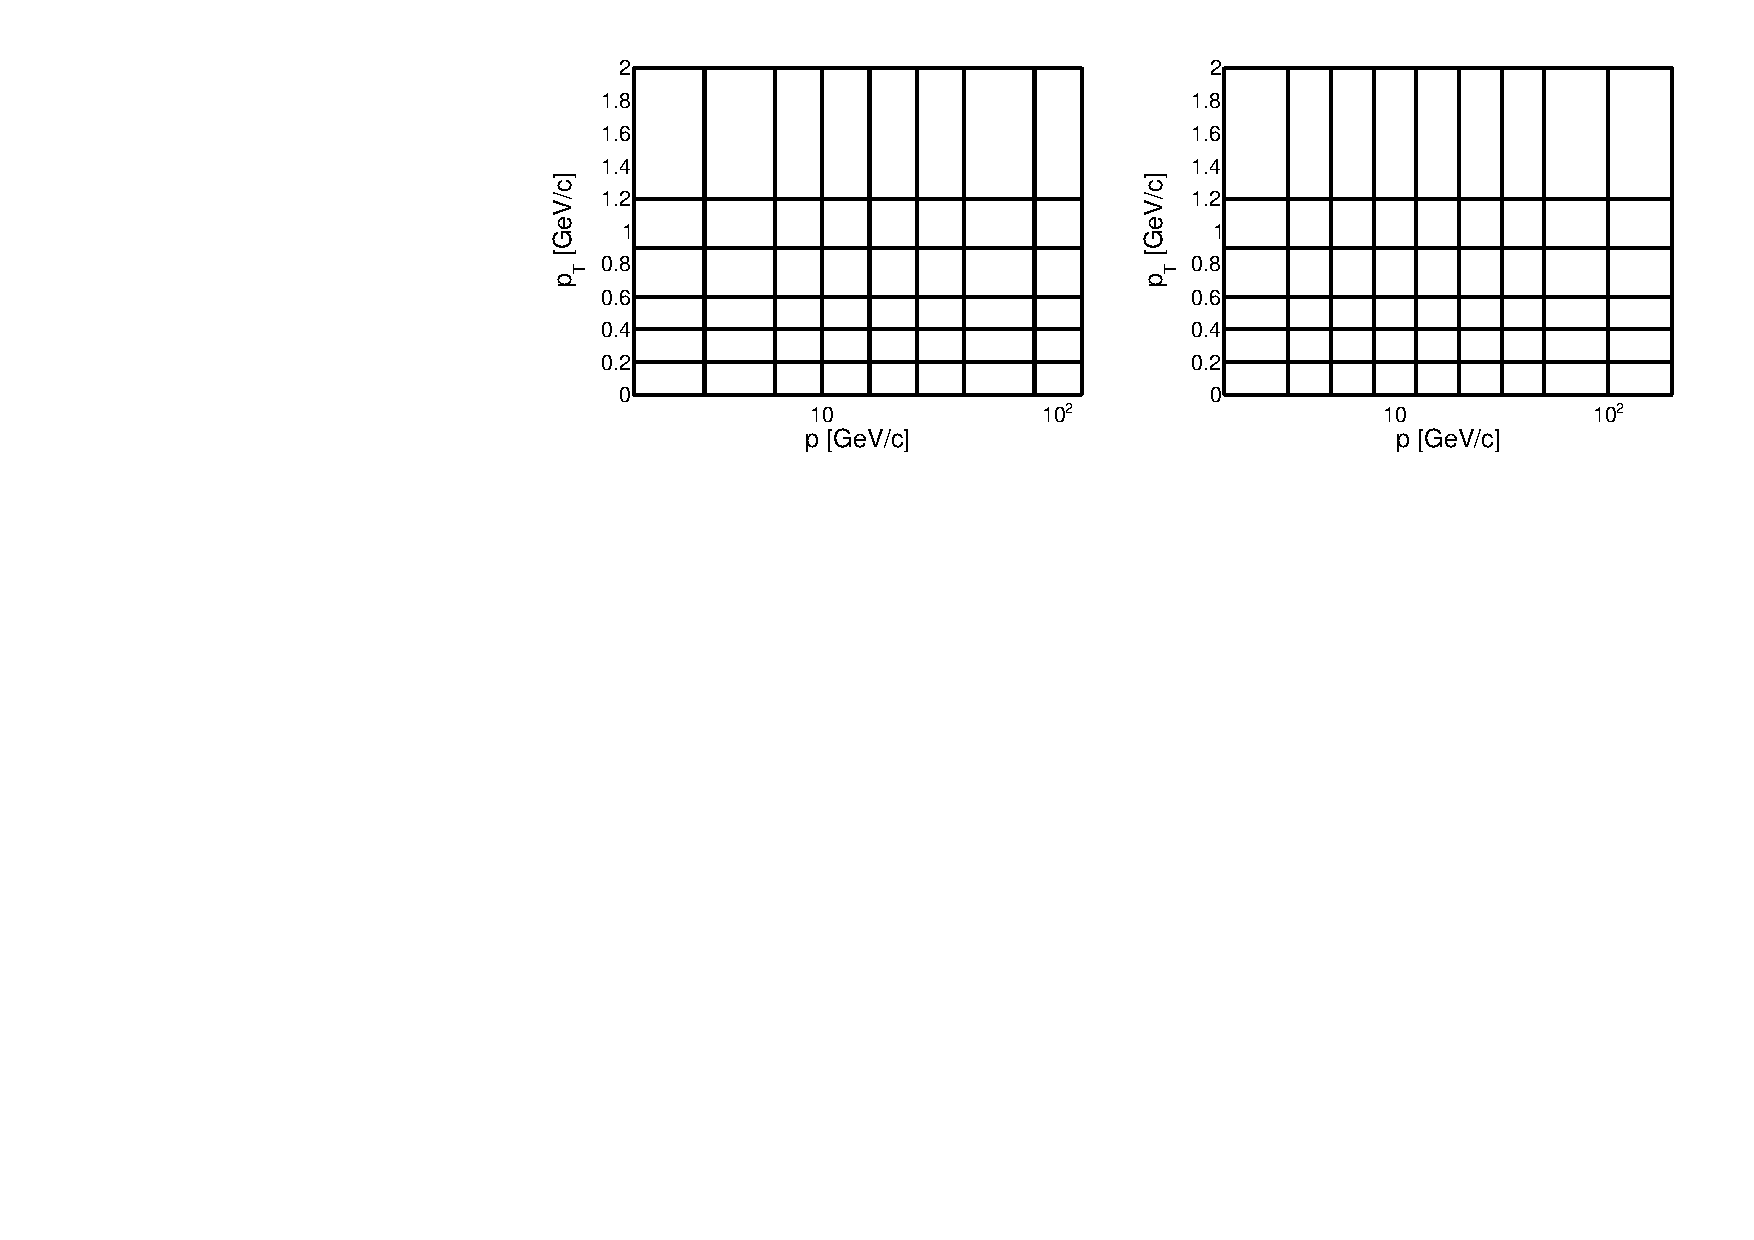
\includegraphics[clip, rviewport=0 0 1 1,width=0.8\textwidth]{V0Binning}
  \caption{}
  \label{fig:hadron:binning:vzero}
\end{figure}


%%%%%%%%%%%%%%%%%%%%%%%%%%%%%%%%%%%%%%%%
\section{Particle identification for the identified spectra}

\note{DONE}

In this section we present the particle identification
analysis for the identified spectra of \pions, \kaons and \protons.
This step is done in a track basis through the \dedx measurements,
being the aim here to determine the fraction of tracks which
correspond to each particle type on every phase space bin.
A brief overview of the \dedx measurements is first given
in~\cref{sec:hadron:dedx:meas}.

The \dedx measurements only allow the particle identification
to be done statistically by fitting
the \dedx distributions with a combination of particle
types. Because of the complicated dependence of the \dedx
distributions on the particle momentum,
features of the measured track (e.g. number of clusters) and
detector properties (e.g. resolution and calibration),
the \dedx fit turns to be very challenging. The first
requirement to perform this step is the development
of a appropriate \dedx model,
which is shown in~\cref{sec:hadron:dedx:model}.

Having in hands the \dedx model, the measured \dedx
distributions can be fitted to determine the particle
fractions. However, the usual large number of
model parameters, added to the
overlap of the \dedx distributions
of different particles in certain regions of momentum,
can make the this fit very hard to perform.
Our fit strategy to overcome these difficulties is shown
in~\cref{sec:hadron:dedx:fit}. A new tool
developed in this work to evaluate the fit performance
and estimate bias and statistical uncertainties of the fit
is presented in~\cref{sec:hadron:dedx:sde}. This
tool is called Simulated Data Emsembles and
it is also used to define cuts on the problematic
phase space bins and to compute correction factors.
Finally, in~\cref{sec:hadron:dedx:fitresults} we show the results
of the particle identification analysis, which include
the particle fractions of \pions, \kaons and \protons
after applying the cuts and corrections.


%%%---------------------------------%%%%
\subsection{\dedx measurements}
\label{sec:hadron:dedx:meas}

\note{DONE}

The \dedx is defined as the energy lost by the
particle to the medium per unit of length. 
In \NASixtyOne the \dedx is measured by the TPCs, which collect the 
freed electrons from the ionization of the gas by the passage of the charged particles.
The determination of the \dedx from the signal recorded at the TPCs requires a complex and
detailed procedure that has been very well established by the \NAFortyNine and \NASixtyOne
experiment along the last decades. Since the detailed description 
is out of the scope of this text, only the general idea and the most important aspects
will be presented in the next paragraphs. More complete and detailed approaches
can be found in Refs.\cite{BlumBook,LeeuwenThesis,GaborVeresThesis}.

Several processes can contribute to the energy loss of charged particle due to
its interaction with atoms of the gas in the TPCs, being the emission of
electrons by ionization the most relevant one. The electrons emitted are
drifted through the chamber and collected in the readout pads, which records
the signal as ADC charges. A set of consecutive charges defines a cluster.
The 3-dimensional position of the cluster is determined by the position
and time distributions in which the charges reach the readout pad.
The position of all clusters are used to define the particle track.

The total charge measured for each cluster is related to the \dedx of each track.
However, numerous detector effects have to be corrected at the cluster level before
grouping the clusters in one unique \dedx value. The simplest correction accounts for
the geometrical differences due to the incident angle of the track in the pad and
the pad widths. More complicated corrections account for differences in the electronic
gain and gas pressure/temperature of the pads, differences in the sector gains and
losses of electrons during the drift in the chambers and in the readout pad.
A detailed description of the correction procedure can be found in Ref.~\cite{AntoniMThesis}.

The track \dedx is then determined by the combination of the corrected 
charges in all clusters. Because of the well known Landau-like shape of the
energy loss probability distribution, the average and the variance
of the measured charges are not well behaved for typical number of clusters
($\sim$ 20-150). This makes the simplest approach, by defining the track \dedx
as the average charge over all cluster, not suitable. 
To overcome this issue and obtain a satisfactory \dedx resolution,
the method of the truncated mean is applied, in which only a subset of the clusters
is selected to compute the average. The selected clusters are defined by ordering
the values of the charge and then selecting the ones inside a given fractional interval.
For the \NASixtyOne experiment it was found the optimal interval being the 50\%
of the clusters with the smallest charges~\cite{GaborVeresThesis}.


%%%---------------------------------%%%%
\subsection{\dedx model}
\label{sec:hadron:dedx:model}

\note{DONE}

To perform the particle identification by fitting the
measured \dedx, a model to describe the \dedx distributions
of different particle types as a function of their
momenta \pp is required. While experiments like
ALICE~\cite{\AlicePaper} and CMS~\cite{\CMSPaper} opt
for modeling the \dedx distributions
with templates~\cite{CorralesMorales:2017zty,Chatrchyan:2012qb},
the \NAFortyNine and \NASixtyOne experiments traditionally adopt
an analytic model, which will also be adopt by us.
Although the model chosen for our analysis is based on previous
studies from \NAFortyNine and \NASixtyOne
collaborations~\cite{LeeuwenThesis,GaborVeresThesis},
it contains particular features that were found
to be the most suitable for the present analysis. 

First, the notation adopted in this text has to be presented
for clarification. The particle types are indexed by
\ipart that can be one of the five options
considered here, $\ipart=e, \pi, K, p, d$. The charges are indexed by
\ich, being that $\ich = +$ or $-$. In addition, the number of
cluster measured in a track is represented by \ncl and the \dedx
is replaced by \eps for shortening.

Because the \dedx is obtained by averaging the measured charge
over a certain number of cluster, it is natural to assume 
the shape of the \eps distribution depends on the \ncl.
To be more precise, the \eps resolution should be 
larger for smaller \ncl and vice-versa. 
Additionally, the mean of the distribution is expected  
to change with the momentum of the particle \pp and the particle type
by following a Bethe-Bloch-like function.

The \eps distribution shape for a given \ncl and \pp
can be well described by an asymmetric Gaussian function.
Thus, the conditional probability density function $f(\eps|\pp,\ncl)$ for a 
\ipart and \ich is written as
\begin{equation}
  f_{\ipart,\ich}(\eps|\pp,\ncl) = \frac{1}{\sqrt{2\pi}\sigma_{\ipart,\ich}} \;
  \exp\left[-\frac{1}{2}\left(\frac{\eps-\mu_{\ipart,\ich}}{\delta \; \sigma_{\ipart,\ich}}\right)^2\right],
  \label{eq:hadron:dedx:model:pdf}
\end{equation}
with
\begin{equation}
  \delta =
  \begin{cases}
    & 1-d, \ \ \ \eps \le \mu_{\ipart,\ich} \\
    & 1+d, \ \ \ \eps > \mu_{\ipart,\ich}, \\
  \end{cases}
  \label{eq:hadron:dedx:model:asymm}
\end{equation}
where $\mu$ is the mode of the distribution, $\sigma$ is the resolution
and $d$ is the asymmetry parameter. The \pp and \ncl dependence is implicit
on the parameters $\mu$ and $\sigma$, as will be explained next.
The mode $\mu$ is related to the mean of \eps (\meaneps) by
\begin{equation}
  \mu_{\ipart,\ich} = \meaneps_{\ipart,\ich} - \frac{\sigma_{\ipart,\ich}}{\sqrt{2\pi}}
  \left[\left(1+d\right)^2 - \left(1-d\right)^2 \right].
  \label{eq:hadron:dedx:model:mu}
\end{equation}

The evolution of \meaneps with \pp is expected to follow
a Bethe-Bloch-like function. In this model, a reference
\meaneps(\pp) curve was defined by a data-based
parametrization using a generic function that is a
variation of the Bethe-Bloch one. The reference value
of \meaneps for a given \pp is denoted by \meanepsbb.
To account for deviations from the reference \meaneps,
our model includes a set of parameters called
\textit{calibration constants}, which are denoted by $X$.
These parameters act as logarithmic shifts of the \meaneps
around \meanepsbb and they can in principle be applied
to each particle and charge separately. However, to reduce the complexity
of the model, it is assumed here one global calibration constant
for each charge that follows the \meaneps of the $\pi$ distribution
and individual calibration constants for the other particle types,
which are common for both charges. In the end, the \meaneps for a
given \ipart and \ich is given by
\begin{equation}
  \meaneps_{\ipart,\ich} =
  \begin{cases}
    & \meaneps_{\ipart}^\text{BB} \; e^{X_{\ipart}^{\ich}} \ \ \ \ \ \ \ \ (i=\pi) \\
    & \meaneps_{\ipart}^\text{BB} \; e^{X_{\pi}^{\ich}} \; e^{X_{\ipart}^{\ich}} \ \ \ (i\neq\pi).
  \end{cases}
  \label{eq:hadron:dedx:model:cal}
\end{equation}
In total the model accounts for 6 calibration constants:
$X_{\pi}^{+}$, $X_{\pi}^{-}$, $X_{e}$, $X_{K}$, $X_{p}$ and $X_{d}$.

The \ncl dependence of the $\sigma$ is assumed to be of the form
$\sigma \sim 1/\sqrt{\ncl}$. $\sigma$ is also assumed to depend
on the \meaneps by a power law relation. Besides that,
the normalization parameter is called
$\sigma_0$ and it is defined separately for each charge ($\sigma_0^{\ich}$).
The final expression for the $\sigma$ is,
\begin{equation}
  \sigma_{\ipart,\ich} = \frac{\sigma_0^{\ich}}{\sqrt{\ncl}} \meaneps_{\ipart,\ich}^{\alpha},
  \label{eq:hadron:dedx:model:sigma}
\end{equation}
in which 3 more parameters are included: $\sigma_0^+$, $\sigma_0^-$ and $\alpha$. 

By combining
the~\cref{eq:hadron:dedx:model:asymm,eq:hadron:dedx:model:mu,eq:hadron:dedx:model:cal,eq:hadron:dedx:model:sigma}
with the~\cref{eq:hadron:dedx:model:pdf}, we obtain the probability density
function of \eps for each particle \ipart and charge \ich. Besides the 6 calibration constants,
the model includes 4 \textit{shape parameters}: $\sigma_0^+$, $\sigma_0^-$, $\alpha$ and $d$.
Altogether there are 10 parameters that can be set free to fit the model
to the measured \eps distributions.


%%%---------------------------------%%%%
\subsection{\dedx fit strategy}
\label{sec:hadron:dedx:fit}

\note{DONE}

The fitting procedure is performed by means of a binned maximum-likelihood method.
In the general case 10 particle fractions (5 particle types and 2 charges) and
10 model parameters are taken as free parameters of the fit. Special cases
in which one or more particle fraction are fixed to zero will be described later.

The \eps data is first divided in bins of $\log_{10}$\eps of width $\Delta\log_{10}$\eps$=0.01$.
The index \ieps will be used to indicate these $\log_{10}$\eps bins.
By using the standard Poissonian probability distribution function in which
$n_{\ich\ieps}$ and $\nu_{\ich\ieps}$ are the observed and expected
number of tracks in a given bin \ieps and charge index \ich,
the log-likelihood function to be maximized is written as
\begin{equation}
  l_0 = 2\ln L = 2\sum_{\ich=+,-}\;\sum_{\ieps=1}^{\neps} \left(\nu_{\ich\ieps} - n_{\ich\ieps}\ln\nu_{\ich\ieps}\right), 
  \label{eq:hadron:dedx:fit:l0}
\end{equation}
where \neps is the number of $\log_{10}$\eps bins and the constant terms were neglected.

The expected number of tracks is computed by using
the \eps model. Since $f_{\ipart\ich}(\eps|\pp,\ncl)$ depends on \pp and \ncl,
it has to be convoluted to the \pp and \ncl distributions
of the measured tracks.
To do that, the measured tracks are first split in
bins of the variables $q = \log_{10}\pp$ and $z = 1/\sqrt{\ncl}$.
These variables were chosen to provide a better sampling
of the data along the bins. The distributions of the
original variables, \pp and \ncl, contain under-sampled
tails which are not suitable for the convolution procedure.

Being \iq and \iz the indexes for $q$ and $z$, the
number of measured tracks in one ($q$,$z$) bin is denoted
by $N_{\iq\iz}$ and the center of the bins are denoted
by $\hat{q}_{\iq}$ and $\hat{z}_{\iz}$. In the next step, the partial
cumulative distribution function in one \ieps bin for each \ipart, \ich,
relative to one ($q$,$z$) bin is computed as
\begin{equation}
  F_{\ipart\ieps\iq\iz} = \int f_{\ipart\ich}(\eps|\hat{q}_{\iq},\hat{z}_{\iz}) d\eps,
\end{equation}
where the limits of the integral are given by the $\log_{10}\eps$
limits of the {\ieps}th bin. Note that the variables $q$ and $z$
were used to evaluate the $f$,
instead of the original \pp and \ncl variables.

The total cumulative distributions $C_{\ipart\ich}$ is computed by summing
the contributions of all ($q$,$z$) bins weighted by its respective
number of measured tracks, as
\begin{equation}
  C_{\ipart\ich} = \sum_{\iq=1}^{\nq} \sum_{\iz=1}^{\nz} N_{\iq\iz} F_{\ipart\ieps\iq\iz},
\end{equation}
where \nq and \nz are the number of \iq and \iz bins, respectively.
The number of mathematical operations in this step
can become very large depending on how large are \nq and \nz,
As a consequence the computing time can be unpraticably long.
On the other hand,
too small number of bins can imply in a undesirable loss of precision
in the results of the fit. Therefore, \nq and \nz were defined
as being approximately the minimum values so there is no negative cost
for the results, which are 5 and 15, respectively.
The limits of the $q$ and $z$ binning were defined automatically
by using the smallest and the largest values found on data.

Finally, the expected number of tracks in one \ieps bin of charge \ich
is computed by summing the contributions of all particle types
in which each one is weighted by its respective fraction $Y_{\ipart\ich}$,
\begin{equation}
  \nu_{\ich\ieps} = \sum_{\ipart=e,\pi,K,p,d} Y_{\ipart\ich} C_{\ipart\ich}.
  \label{eq:hadron:dedx:fit:exp}
\end{equation}
This expression is then combined to the one in~\cref{eq:hadron:dedx:fit:l0}
to determine $l_0$.

In addition to $l_0$, the final log-likelihood function
to be maximized, $l$,
will also include terms from Gaussian constraints for the model
parameters. These are quadratic terms of the
form $\left[(b-b_c)/\sigma_b\right]^2$ added to $l$,
where $b$ can be one of the model parameters and 
$b_c$ and $\sigma_b$ are its
estimated mean value and standard deviation, respectively.
It is important to constrain the model parameters because
the number of tracks in the \eps distribution
can be eventually very low for a number of phase space bins.
In these cases, the lack of statistics combined to
the large number of free parameters can make the fit
impracticable if the constraints are not applied.
Furthermore, the constraints are also important
even for bins with large statistics,
in which the proximity of the position of \eps distributions
for two particles can create a partial degeneracy
between the respective calibration constants,
and consequently
generate large instabilities in the fitting procedure.

The $b_c$ and $\sigma_b$ were
estimated by performing the fit without adding
the Gaussian constraints and evaluating
the mean and standard deviation of the fitted parameters
with the phase space bins in which the fit converged properly.
By construction the mean value of the calibration constants
are zero. An additional term was included to constrain the
difference between global calibration constants for both
charges ($X_{\pi}^+$ and $X_{\pi}^-$) to avoid solutions
in which one of the charges is largely shifted
with relation to the other.
The sum of all model parameters constrain terms are given by,
\begin{multline}
  c_m = \left(\frac{X_{\pi}^+}{0.01}\right)^2+\left(\frac{X_{\pi}^-}{0.01}\right)^2+
  \left(\frac{X_{e}}{0.005}\right)^2+\left(\frac{X_{K}}{0.005}\right)^2+
  \left(\frac{X_{p}}{0.005}\right)^2+\left(\frac{X_{\pi}^+-X_{\pi}^-}{0.01}\right)^2+\\
  \left(\frac{\sigma_0^+-0.4}{0.2}\right)^2+\left(\frac{\sigma_0^--0.4}{0.2}\right)^2+
  \left(\frac{\alpha-0.75}{0.1}\right)^2+\left(\frac{d-0.05}{0.03}\right)^2
  \label{eq:hadron:dedx:fit:cm}
\end{multline}

Because of the very low fraction of deuterons,
the deuteron fractions ($Y_{d,+}$ and $Y_{d,-}$)
may not be well determined by the fit. As a consequence, we
observed that for a number of phase space bins the fitted deuteron
fraction does not make physical sense and then the fractions
of other particles turns to be biased. To avoid this problem,
the parameters $Y_{d,+}$ and $Y_{d,-}$ were also
constrained. Their mean value is set
to zero and their standard deviation to 0.02.
Since the fraction for deuterons is not expected
to be much larger than 0.01 in any case, the constraint
is assumed not to bias the fit, being important
only to forbid non-physical results. The term added
is given by
\begin{equation}
  c_d = \left(\frac{Y_{d,+}}{0.02}\right)^2+\left(\frac{Y_{d,-}}{0.02}\right)^2.
  \label{eq:hadron:dedx:fit:cd}
\end{equation}

The final log-likelihood function to be maximized is then
computed as
\begin{equation}
  l = l_0+c_m+c_d,
  \label{eq:hadron:dedx:fit:l}
\end{equation}
where $l_0$, $c_m$ and $c_d$ are given
by~\cref{eq:hadron:dedx:fit:l0,eq:hadron:dedx:fit:cd,eq:hadron:dedx:fit:cm}.

The maximization of $l$
was performed by using the MINUIT package~\cite{James:1975dr}.
When fitting models with large number of free parameters,
it is important to define suitable starting parameters
to assure the convergence of the maximization and
reduce the computing time needed for that.
The starting parameters here are defined by means of
preliminary fitting phases, in which a simplified fitting
procedure is performed. In the first phase, only the model
parameters are set free for the likelihood maximization
and the fractions are computed in each step,
for a given set of model parameters, by an
analytic minimization of the $\chi^2$.
In the second phase, the model parameters are fixed
to the values obtained by the solution of the first phase
and the fractions are obtained by the likelihood fit,
which is performed separately for each charge.
The starting parameters for the main fit is given by
the model parameters obtained in the first phase and the
fractions obtained in the second phase.

To simplify the fit and reduce the uncertainties on the
fraction of particle of interest (\pions, \kaons and \protons),
the fractions of deuterons and electrons were fixed to zero
for bins with momentum above a certain limit. These limits were
defined based on their asymptotic behavior observed by performing
the fit setting all fractions free and the values are 3 and 70 \GeVc
for deuterons and electrons, respectively. 

The sub-sets of tracks defined as RST and WST were fitted
separatly (see~\cref{sec:hadron:trackselection} for the definitions).
This is motivated by the fact that, for the same phase space
interval, these two types of tracks are detected by
different parts of the TPCs. Since the model parameters,
mainly the calibration constants, are related to
detector features, it is expected that the solutions
of RST and WST present differences on the fitted
parameters.

Since the number of tracks measured with the target removed is much
smaller than with target inserted, the
fitting procedure described above is not suitable for the
target removed dataset. The complexity of the model
(or the large number of free parameters) combined with
the poor statistics would strongly reduce the precision of
the results, or even prevent the convergence of the maximization
algorithm. To overcome this problem, the particle fractions
from the target removed data were obtained by means of
a $\chi^2$ minimization, in which all the model parameters
were fixed to the value obtained from the target inserted
dataset fit. Since the model prediction is linear on
the particle fraction, the minimization was performed
analytically. 

%%%---------------------------------%%%%
\subsection{\dedx fit results}
\label{sec:hadron:dedx:fitresults}

\note{DONE}

Examples of the fitted \dedx distributions are shown
in~\cref{fig:hadron:dedx:fit:dist158,fig:hadron:dedx:fit:dist350}.
Although the fit was performed by the maximum likelihood method,
the \redchisq can still be used to evaluate the goodness of fit.
In~\cref{fig:hadron:dedx:fit:chi},
we show the \redchisq distributions.
One can see that the \redchisq follow the expected trend,
with average value around 1 and few bins with \redchisq$\sim2-2.5$.
Therefore, we conclude that the \dedx model
provides a good description of the data.

%%%%%%%%%%% DIST %%%%%%%%%%%%%%%%%%
\begin{figure}
  \centering
  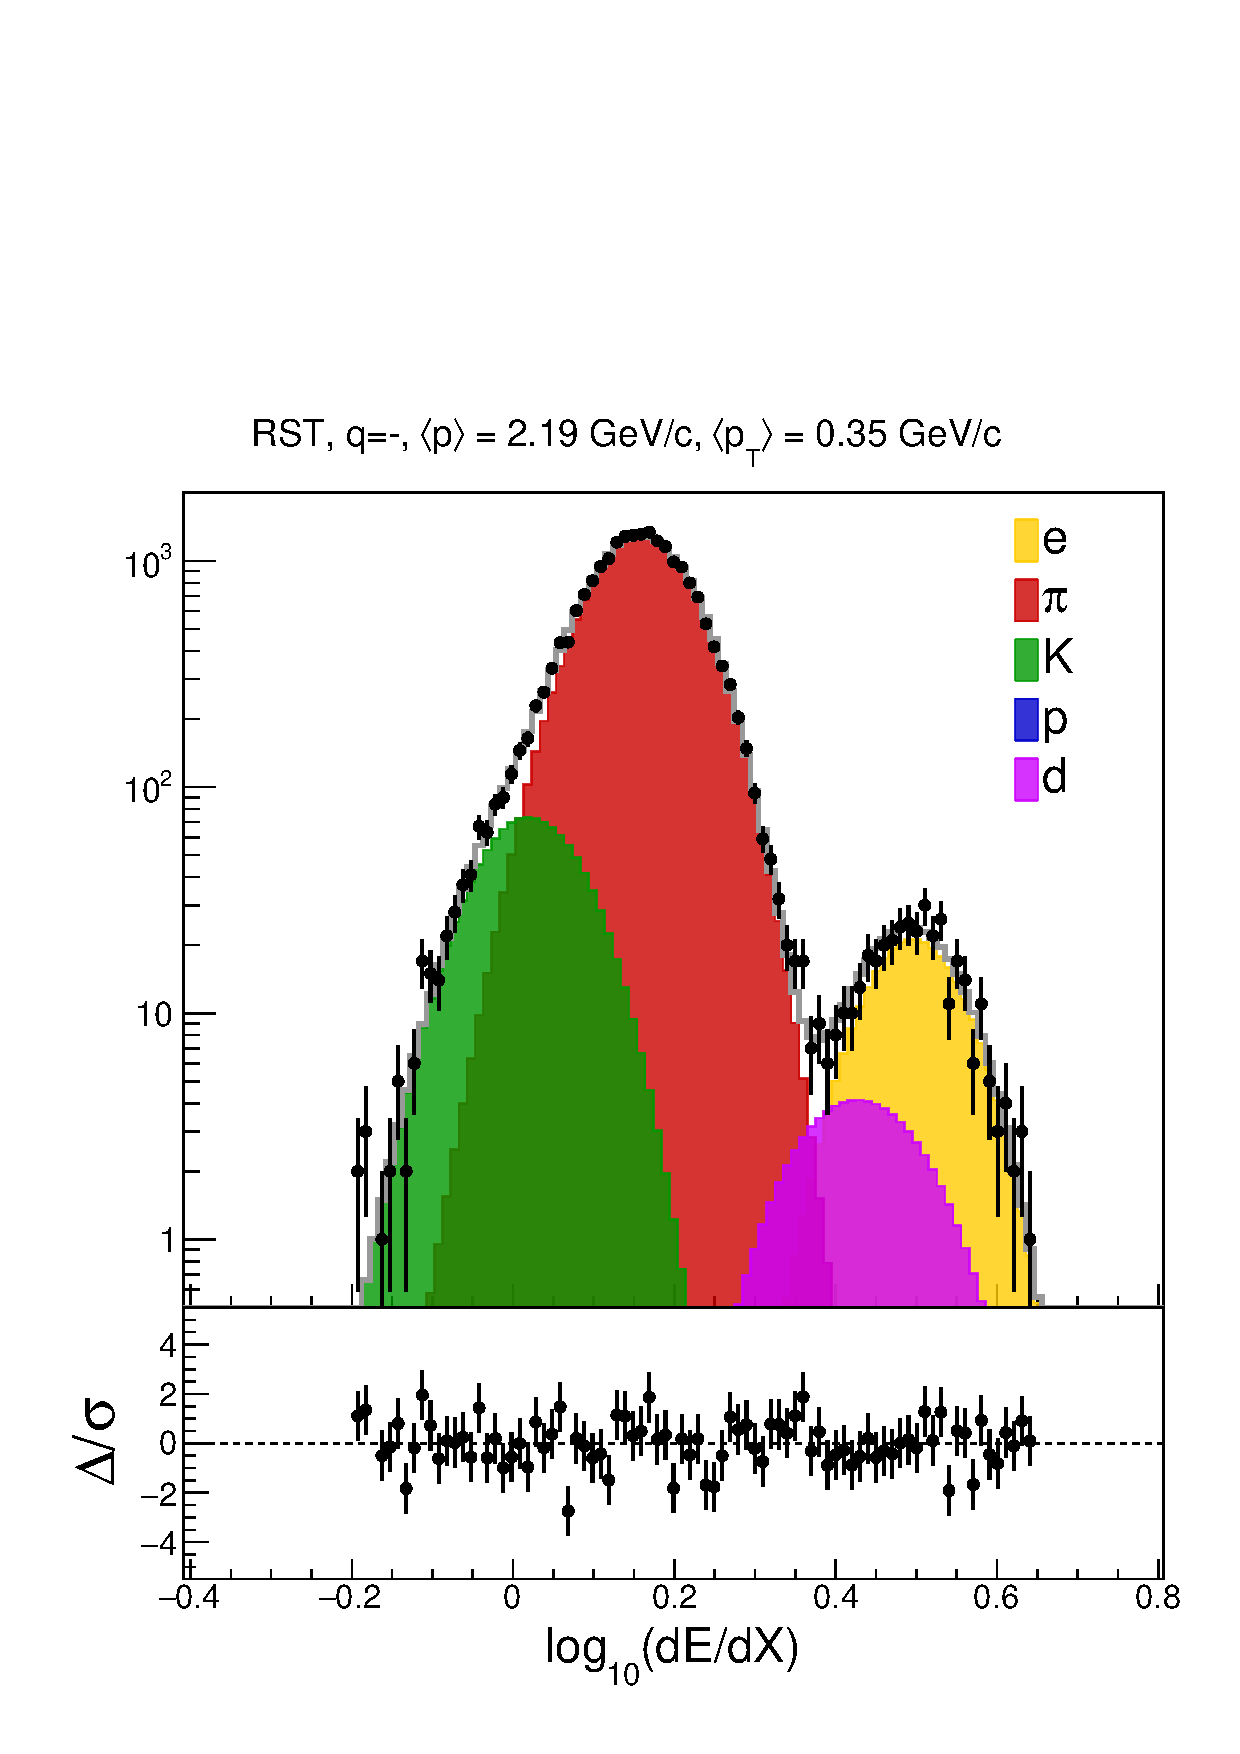
\includegraphics[clip, rviewport=0 0 1 1,width=0.4\textwidth]{dedx/dist_158_v0_c0_x13_y3}
  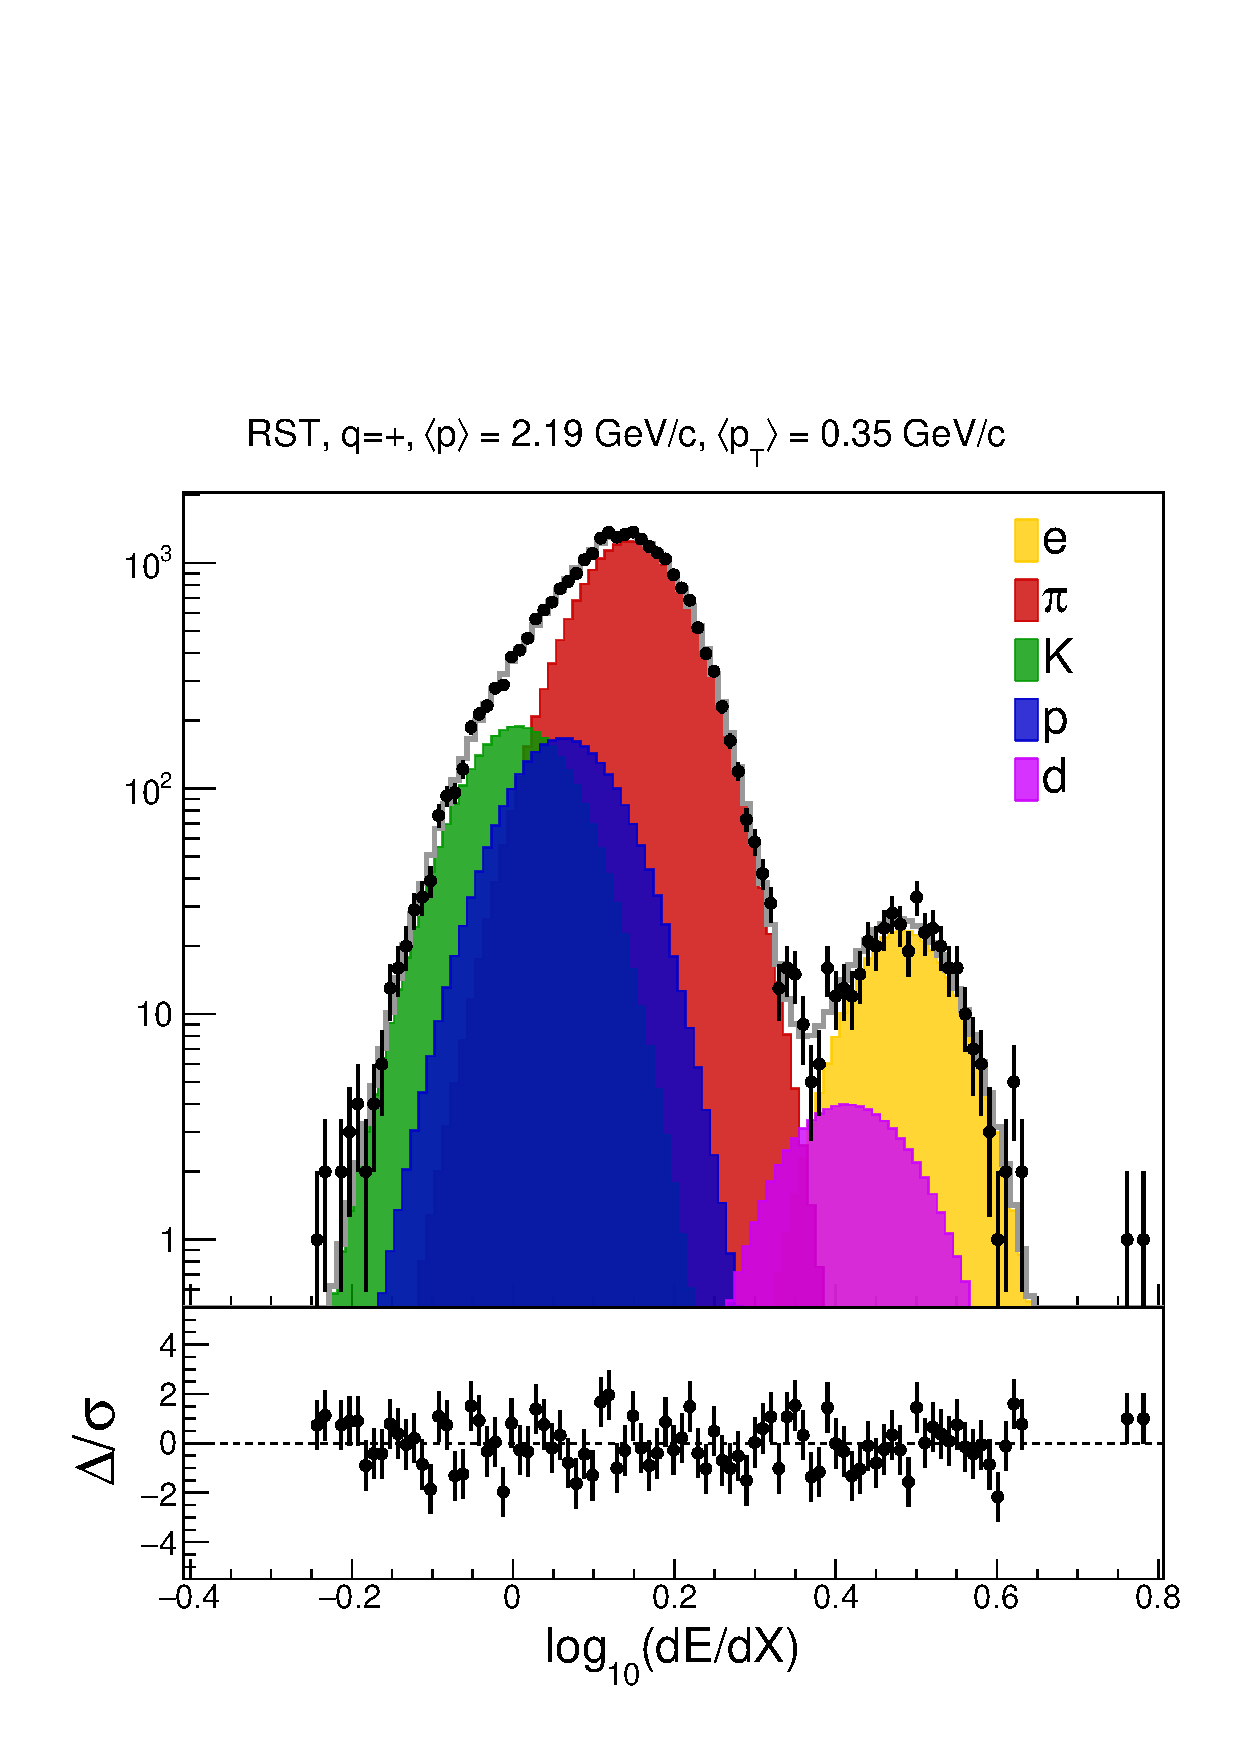
\includegraphics[clip, rviewport=0 0 1 1,width=0.4\textwidth]{dedx/dist_158_v0_c1_x13_y3}

  \vspace{0.5cm}
  
  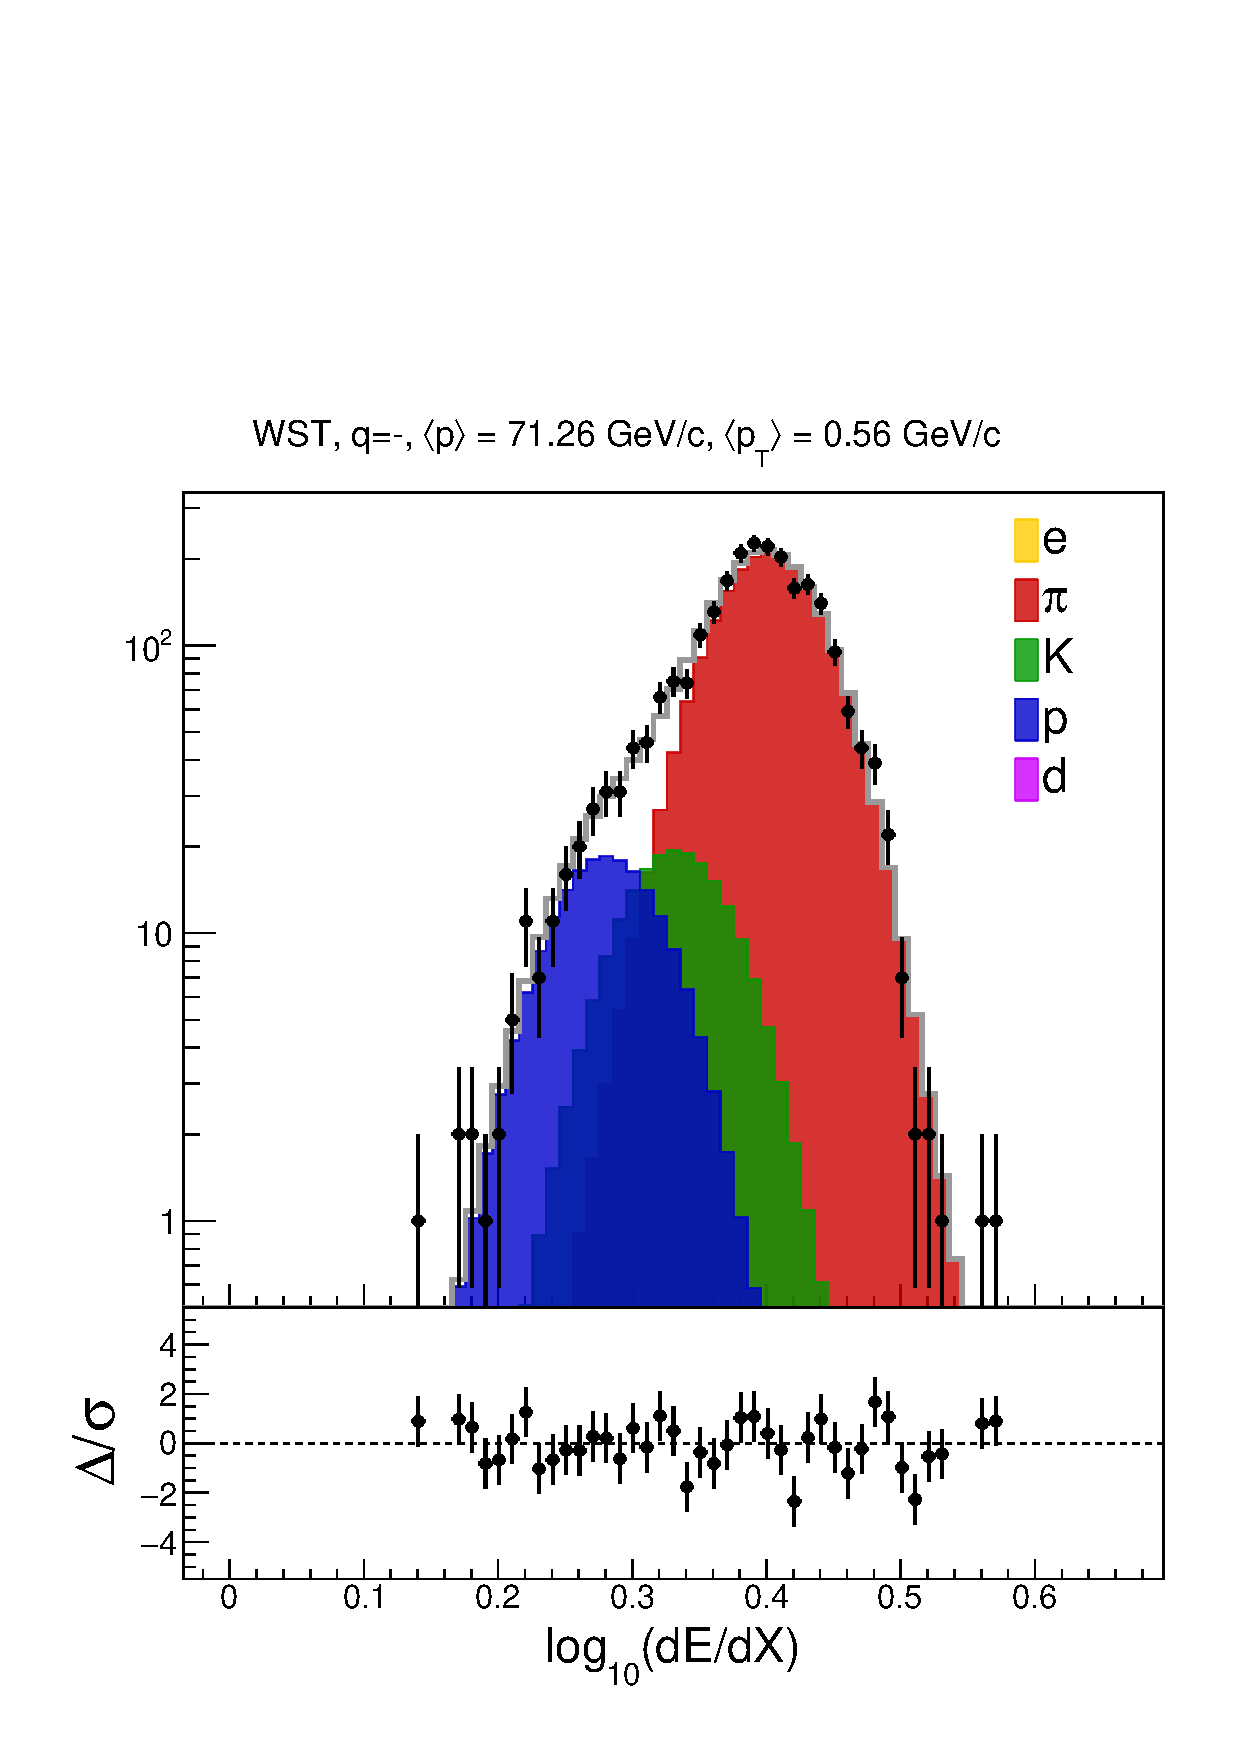
\includegraphics[clip, rviewport=0 0 1 1,width=0.4\textwidth]{dedx/dist_158_v1_c0_x29_y5}
  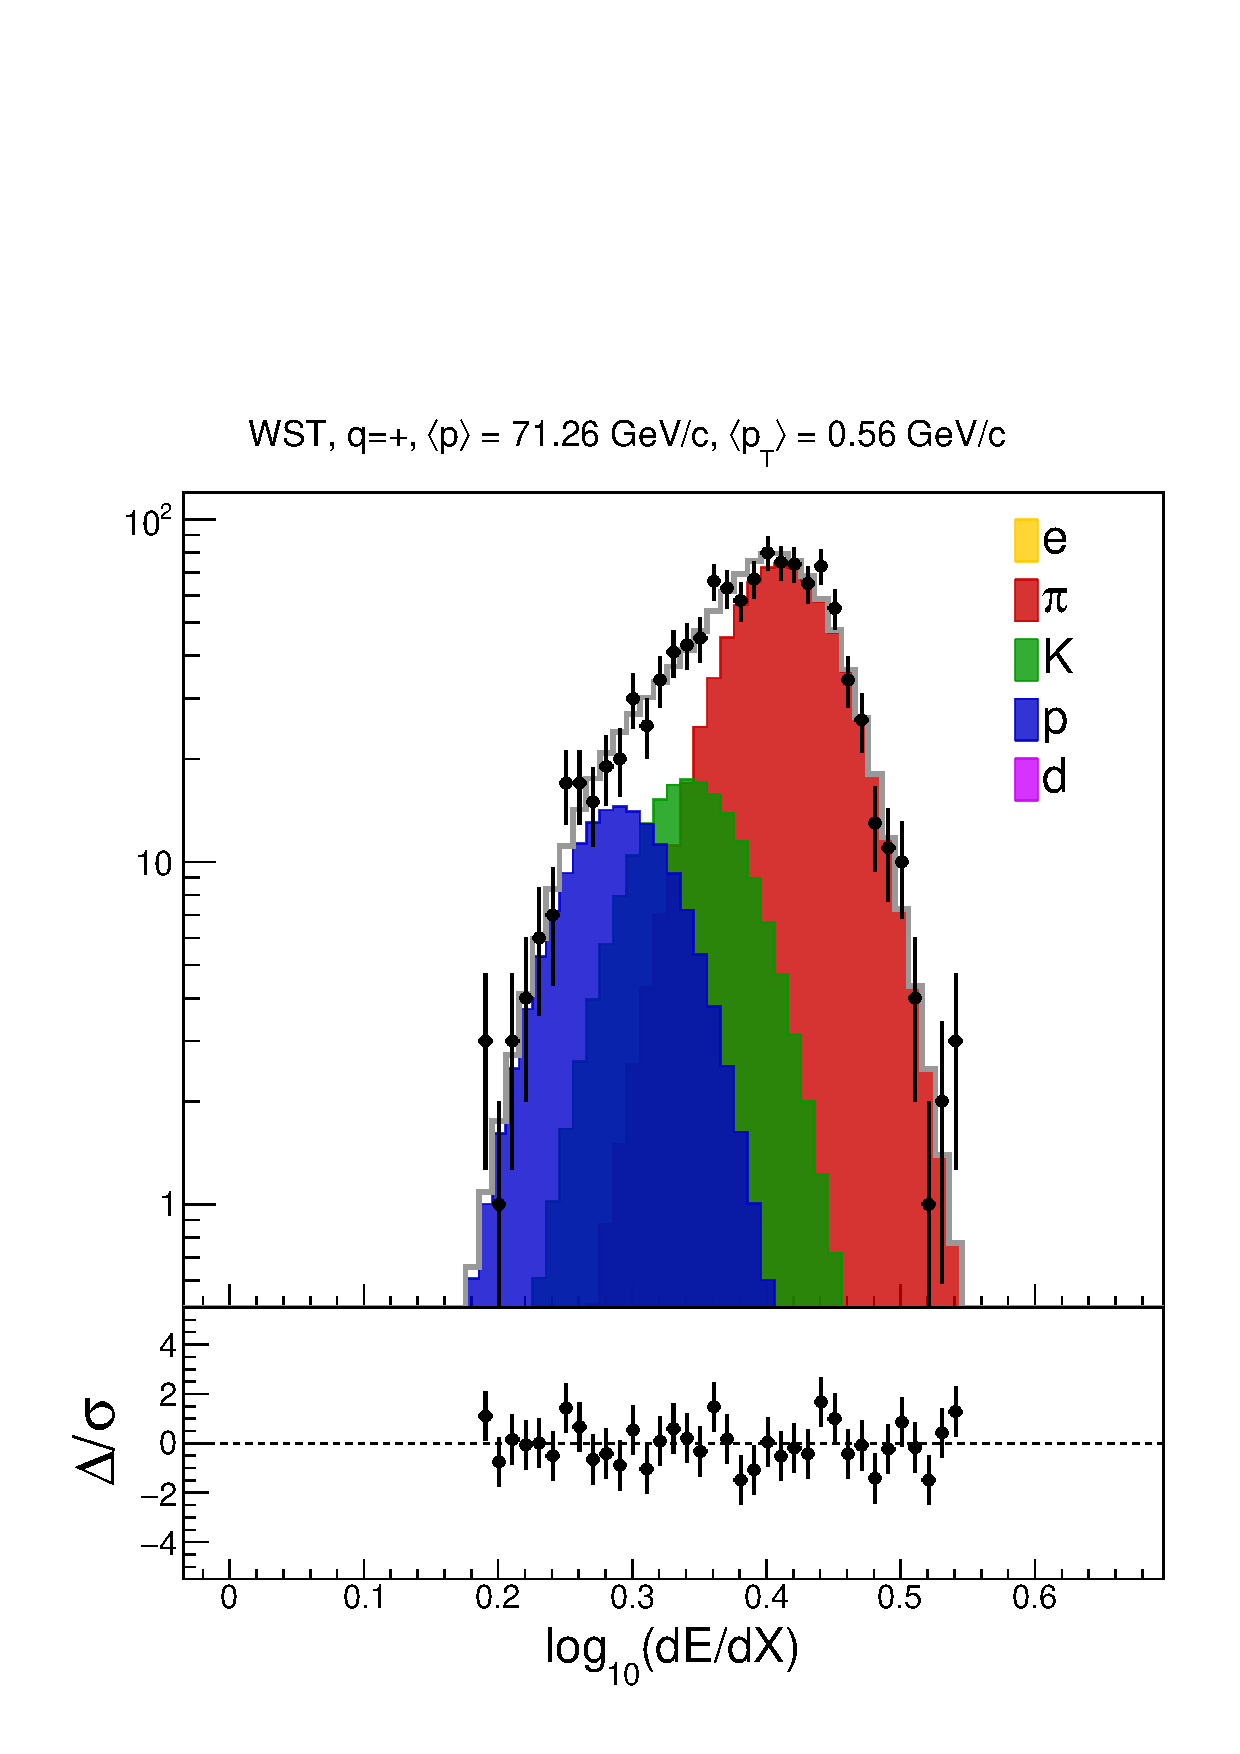
\includegraphics[clip, rviewport=0 0 1 1,width=0.4\textwidth]{dedx/dist_158_v1_c1_x29_y5}
  
  \caption{Examples of the fitted \dedx distributions from the 158 \GeVc dataset.}
  \label{fig:hadron:dedx:fit:dist158}
\end{figure}


%%%%%%%%%% CHI SQ %%%%%%%%%%%%%%
\begin{figure}
  \centering
  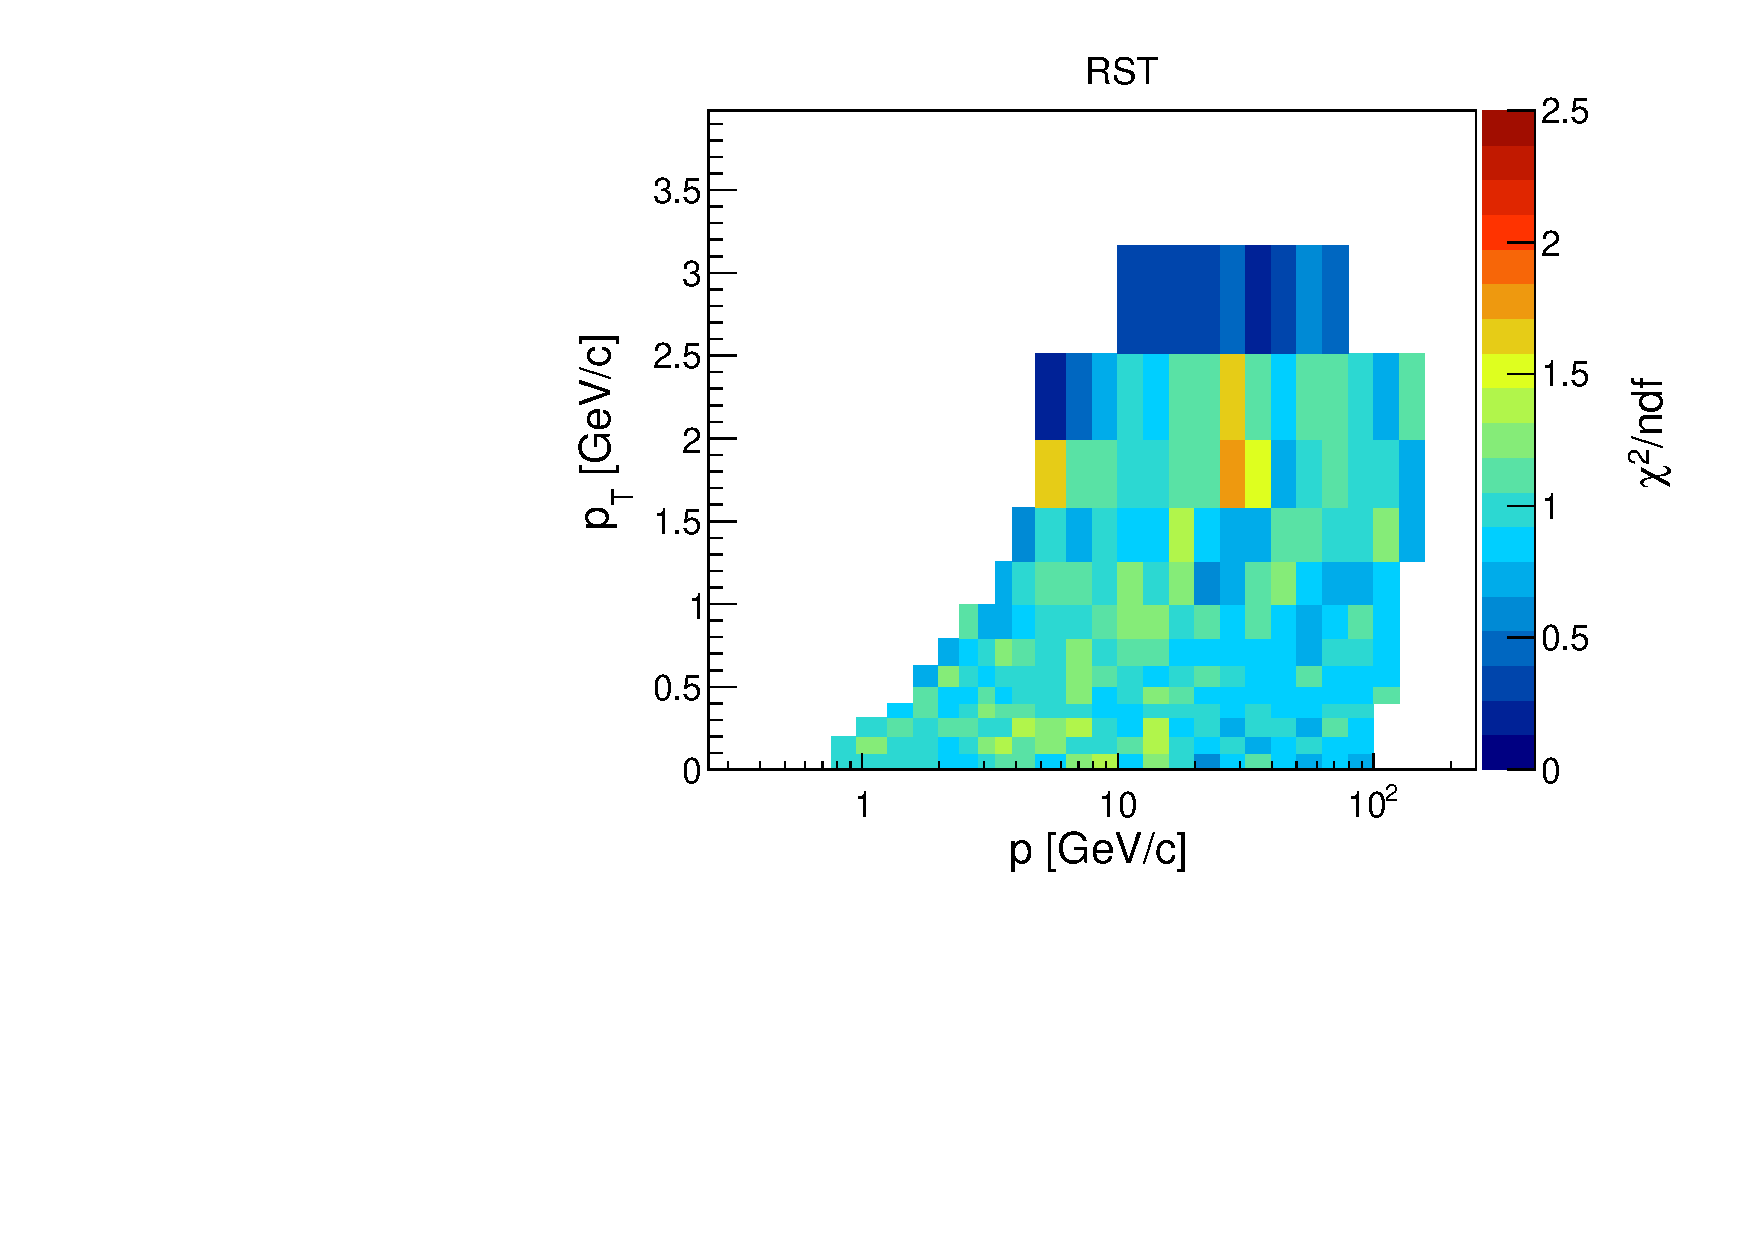
\includegraphics[clip, rviewport=0 0 1 1,width=0.4\textwidth]{dedx/chisq_158_v0}
  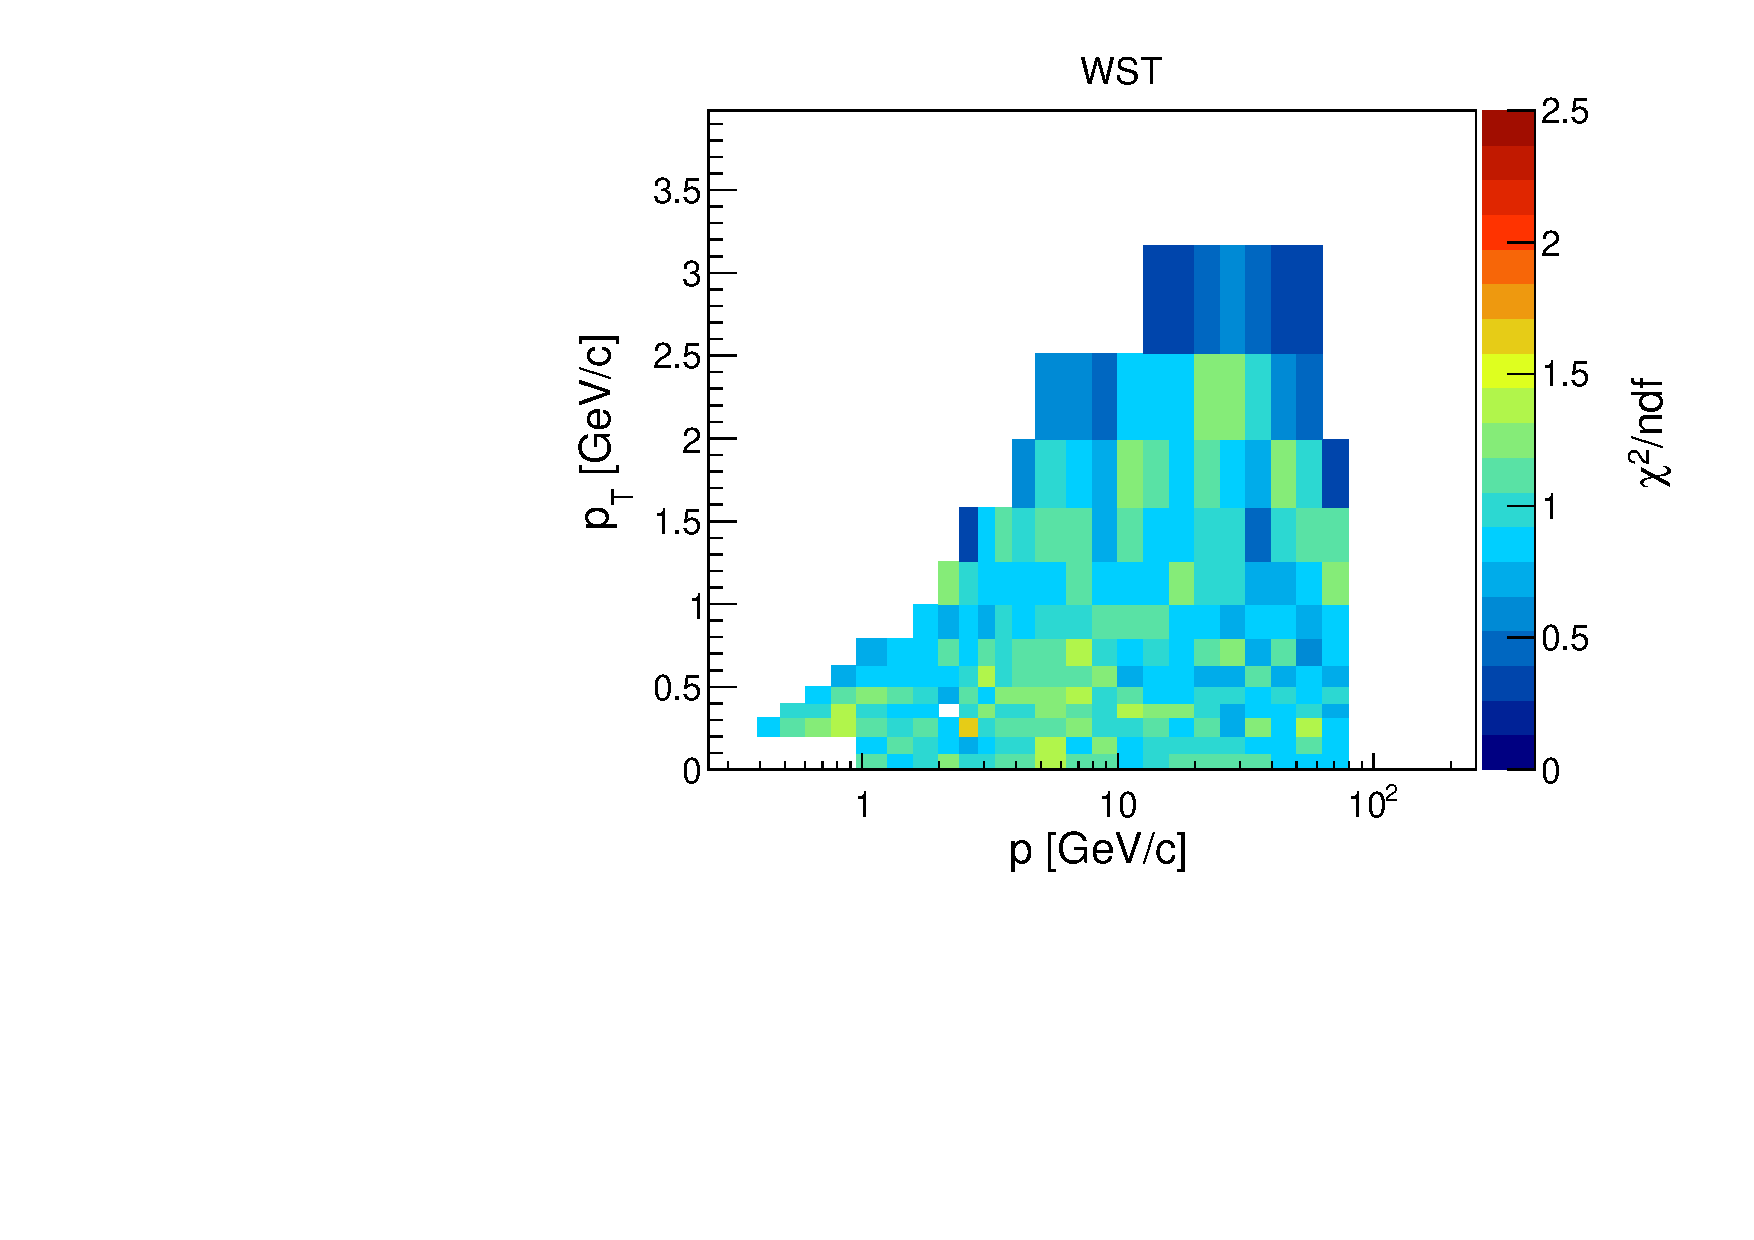
\includegraphics[clip, rviewport=0 0 1 1,width=0.4\textwidth]{dedx/chisq_158_v1}

  \vspace{0.5cm}

  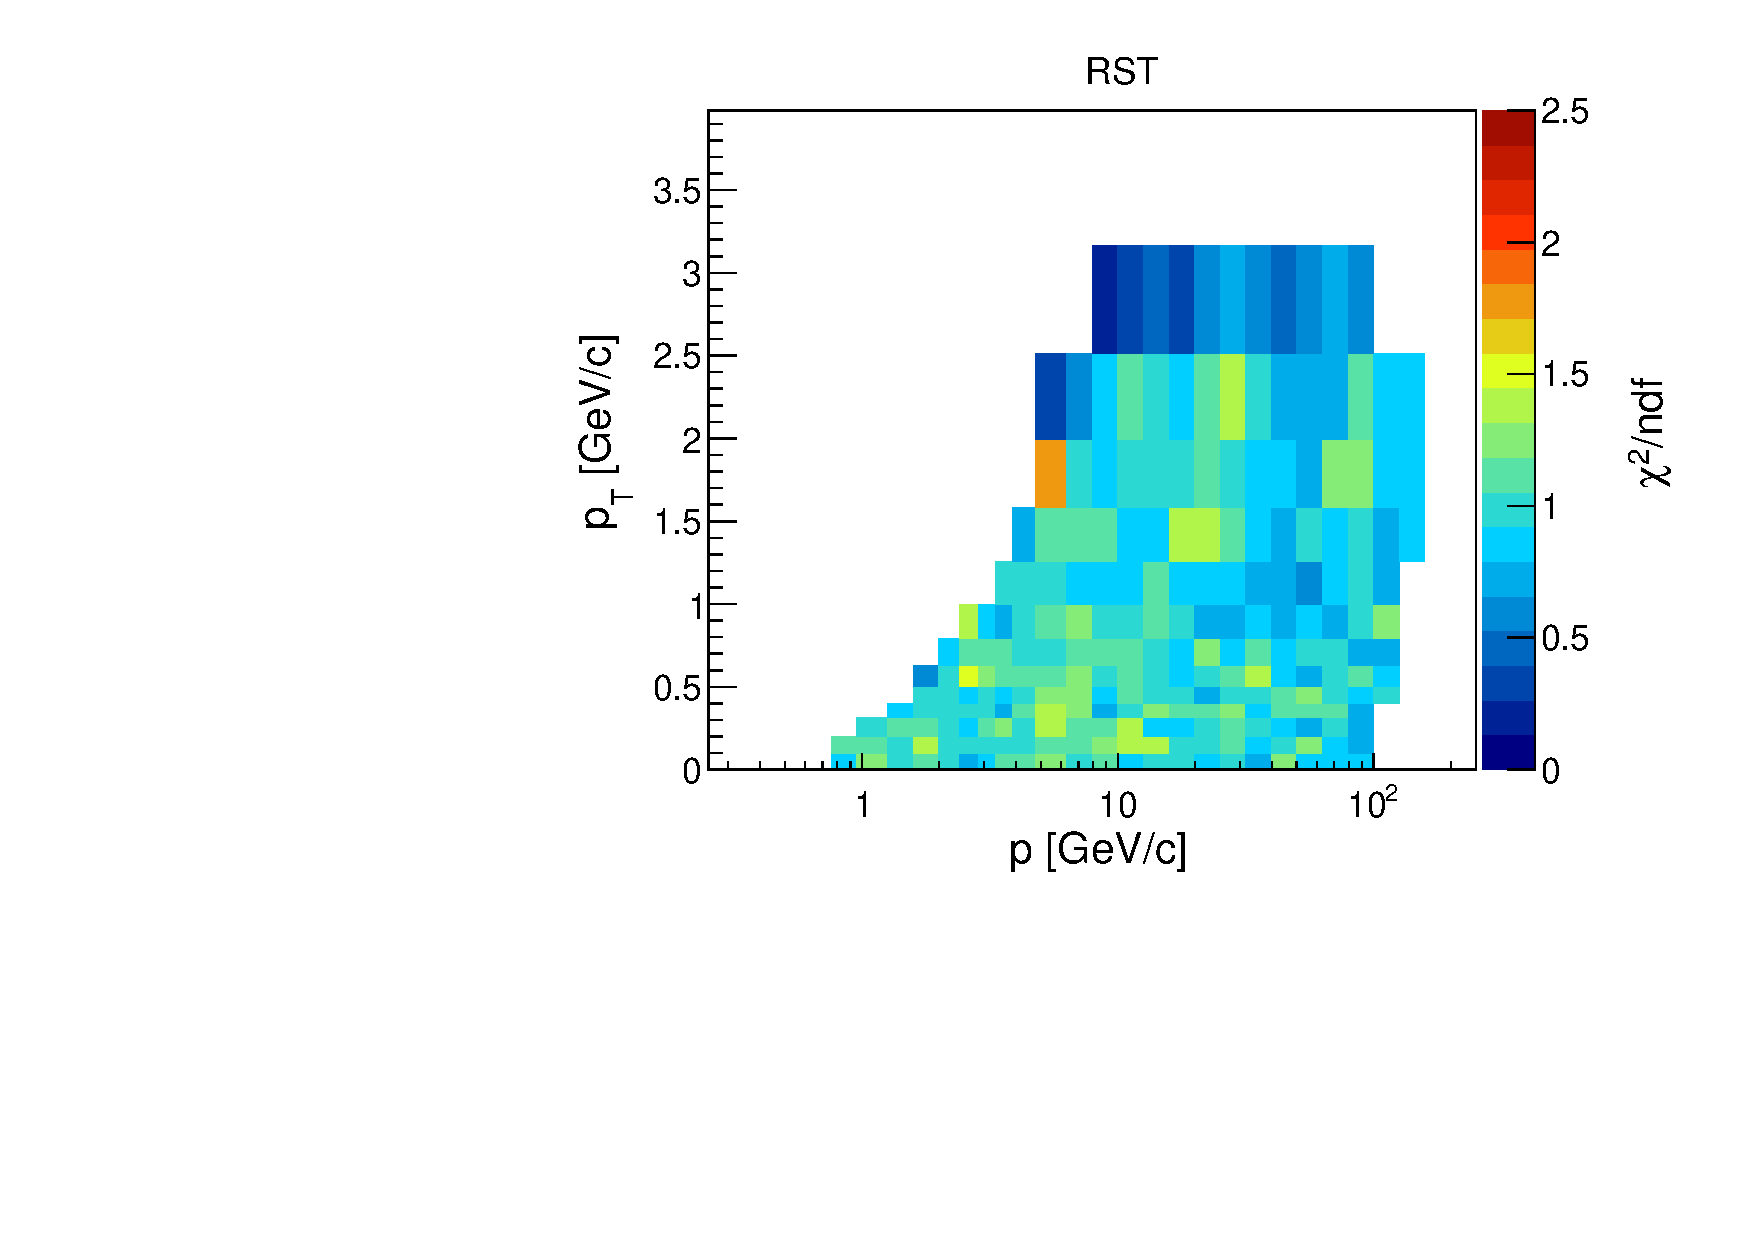
\includegraphics[clip, rviewport=0 0 1 1,width=0.4\textwidth]{dedx/chisq_350_v0}
  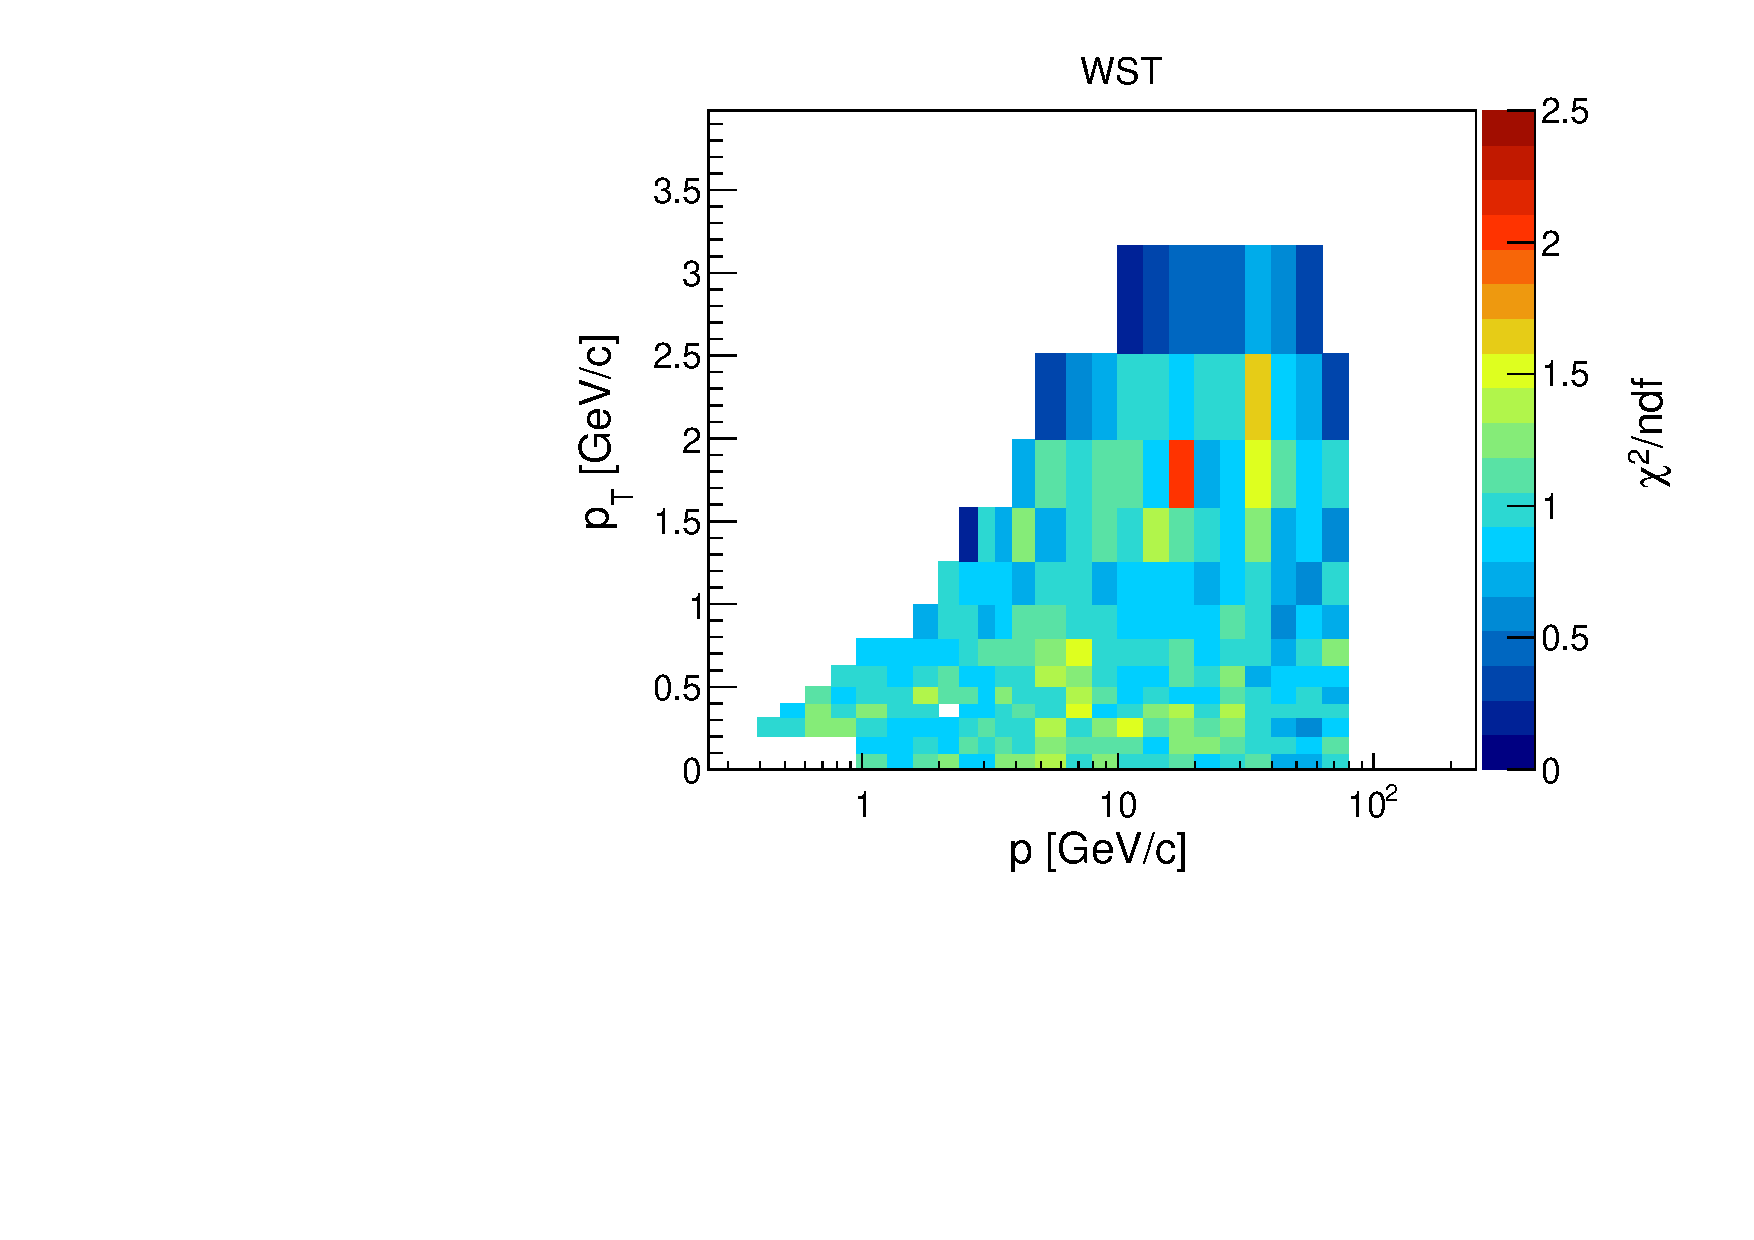
\includegraphics[clip, rviewport=0 0 1 1,width=0.4\textwidth]{dedx/chisq_350_v1}
 
  \caption{\redchisq of the \dedx fit from the 350 \GeVc dataset.}
  \label{fig:hadron:dedx:fit:chi}
\end{figure}

Examples of the calibration constants obtained by the fit of the
RST and 158 \GeVc dataset are shown in~\cref{fig:hadron:dedx:fit:cal158r}.
The remaining cases are shown
in~\cref{fig:hadron:dedx:fit:cal158w,fig:hadron:dedx:fit:cal350r,fig:hadron:dedx:fit:cal350w}.
As expected, in general they exhibit small deviation
from zero. Besides that, we can see
that they show a systematic dependence with the phase space region,
in particular with \pT. This dependence makes evident that there is indeed
small differences on the \dedx calibration in different regions of the TPCs.
Therefore we conclude that a single Bethe-Bloch parametrization,
without the calibration constants, would not provide
a suitable description of the \dedx data. Furthermore,
the RST and WST results also exhibit different behavior,
which proves the necessity of performing the \dedx
fit separately for both datasets.

%%%%%%%%%% CAL %%%%%%%%%%%%%%
\begin{figure}[!ht]
  \centering
  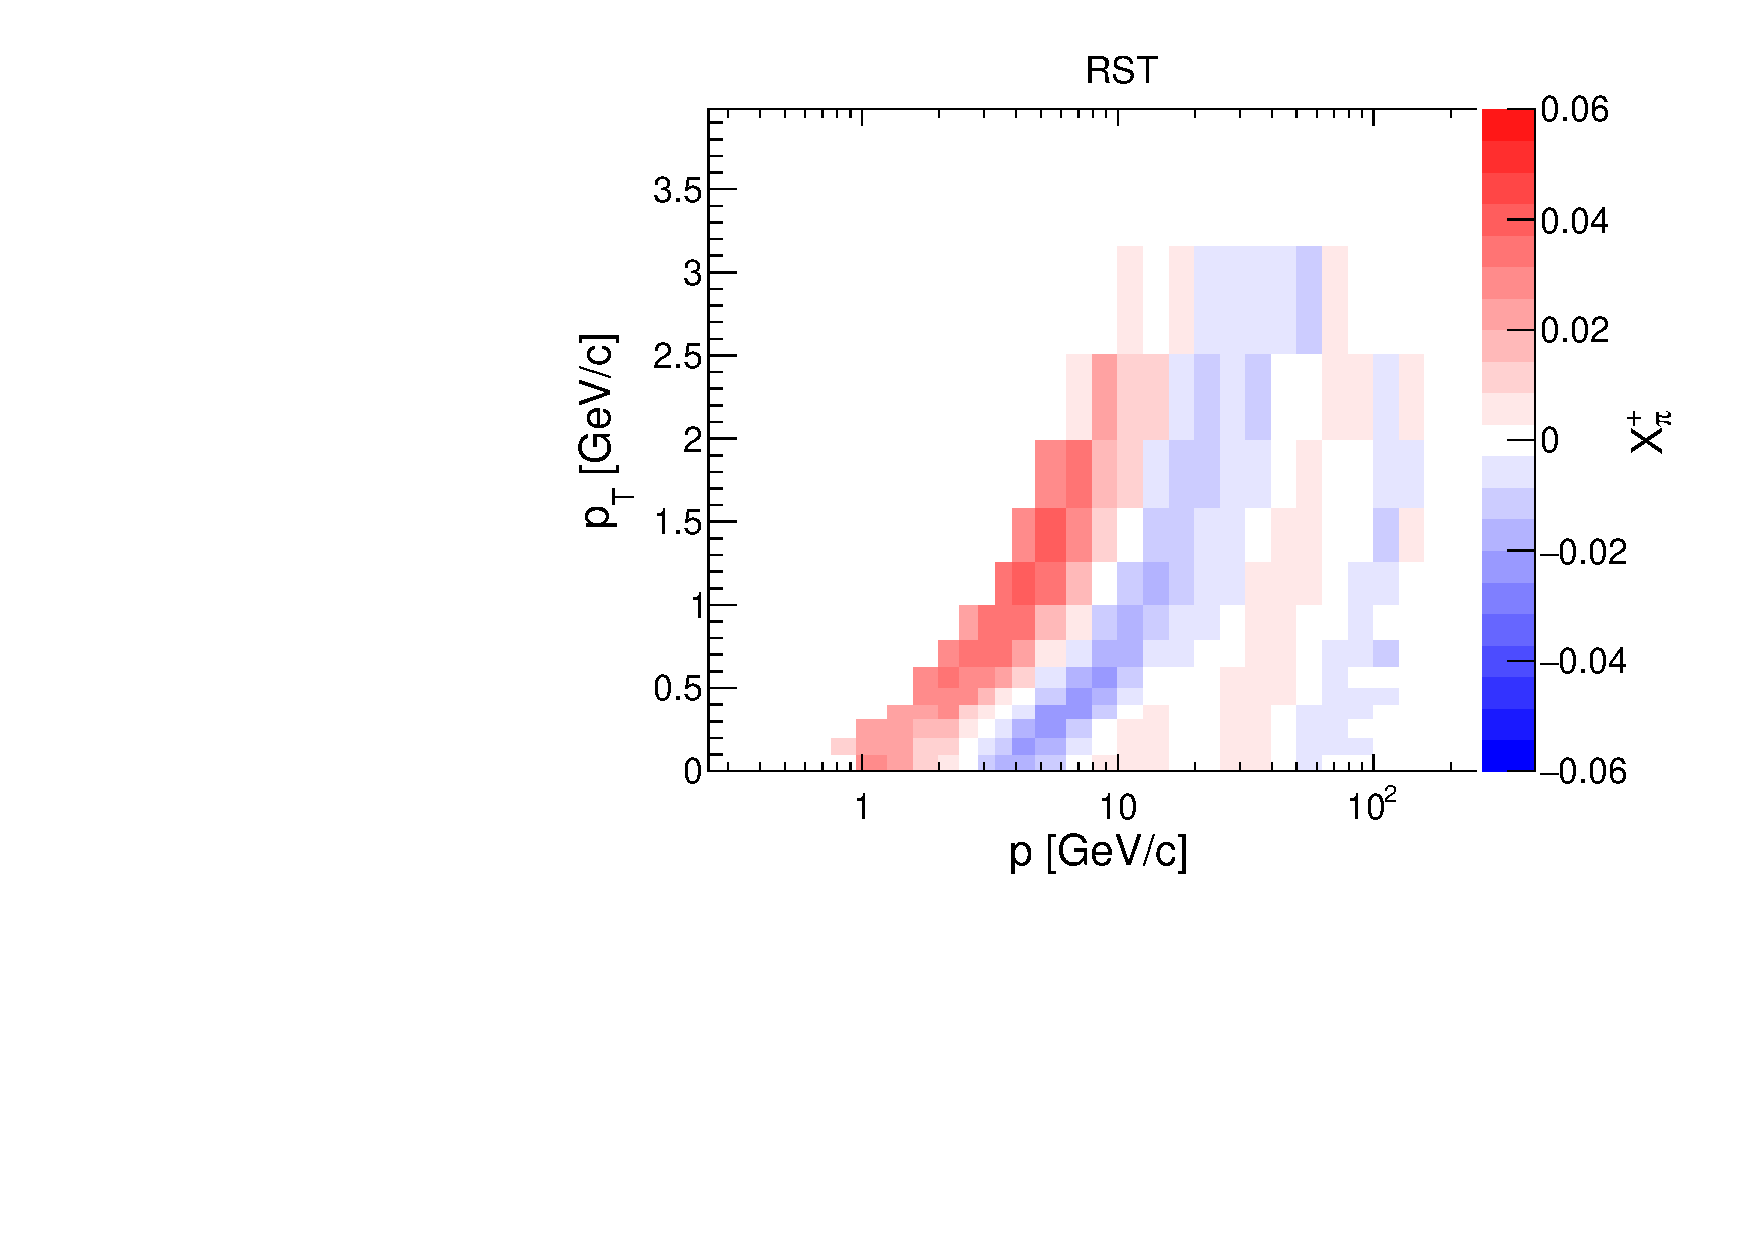
\includegraphics[clip, rviewport=0 0 1 0.94,width=0.4\textwidth]{dedx/model_158_v0_m0}
  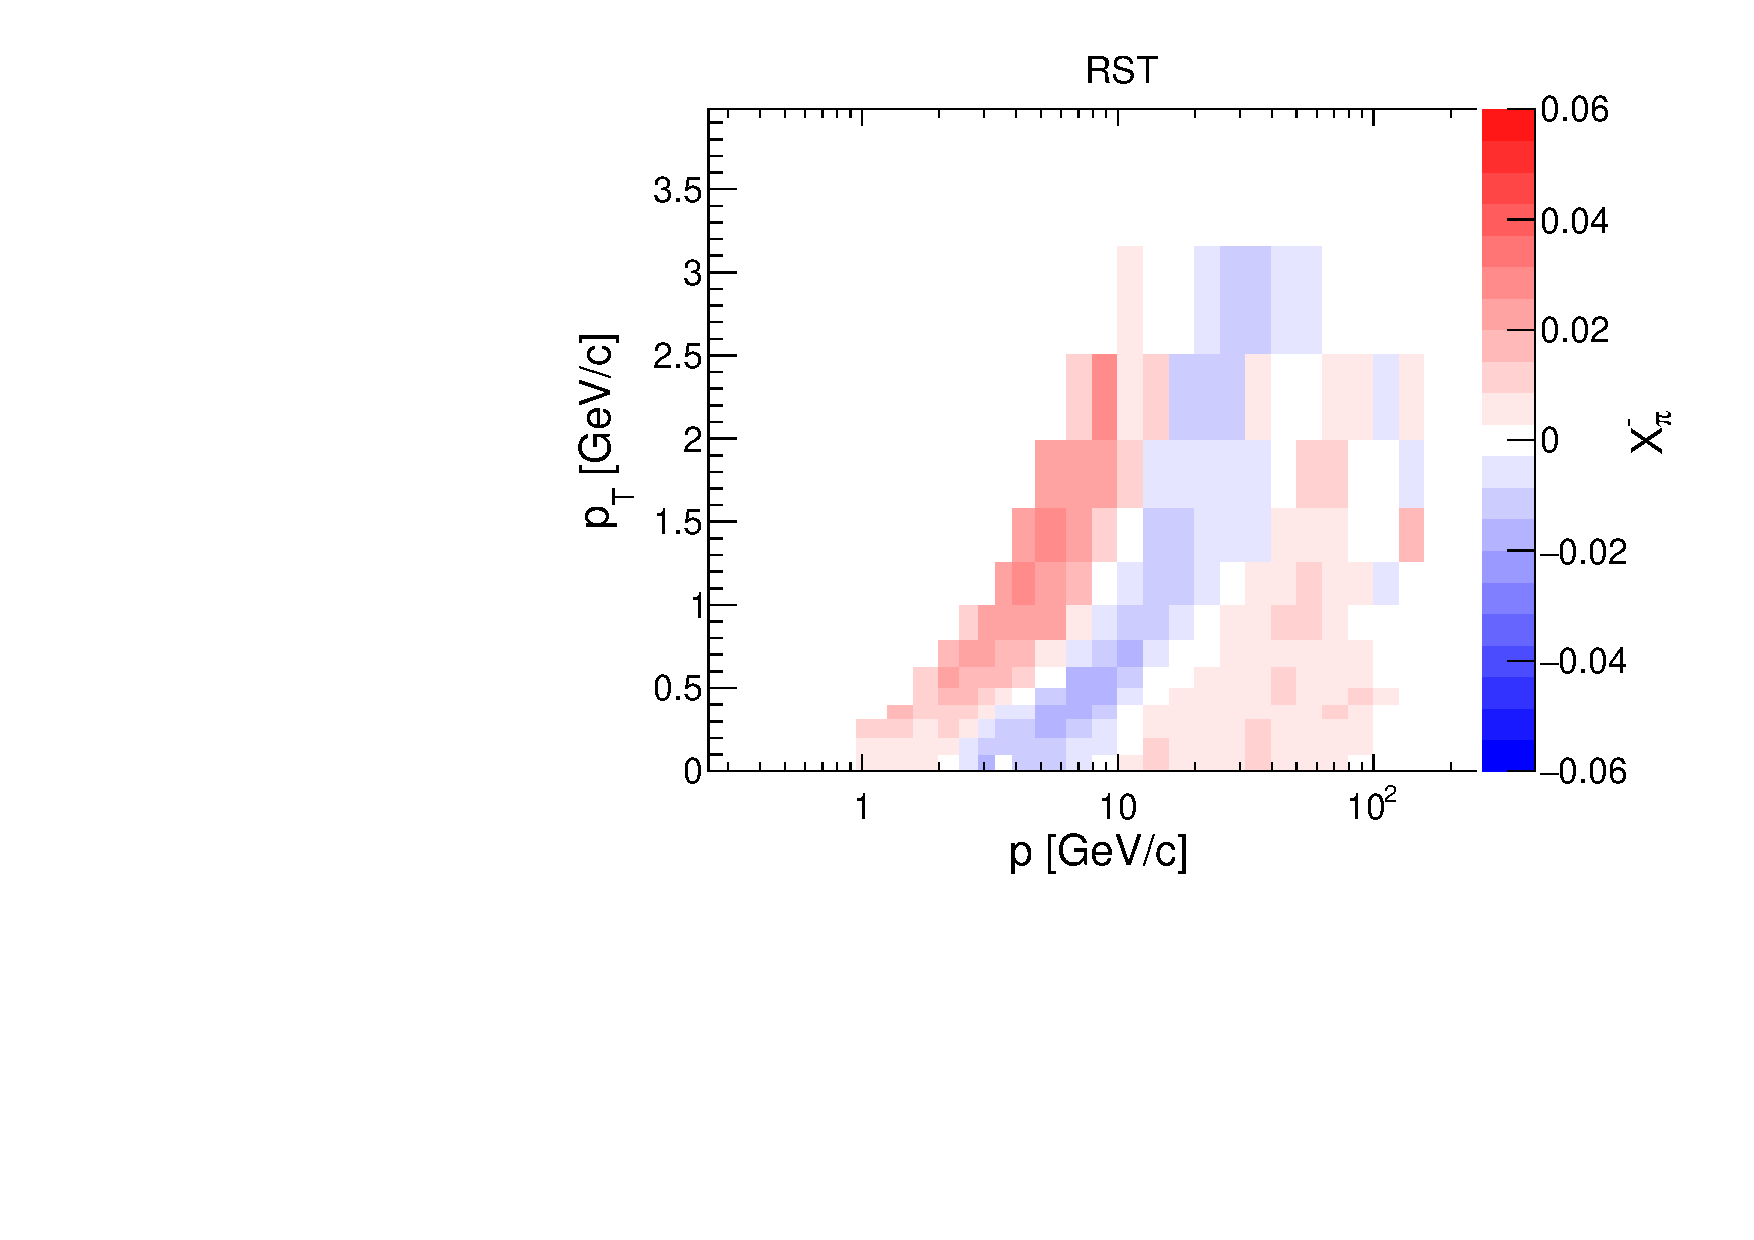
\includegraphics[clip, rviewport=0 0 1 0.94,width=0.4\textwidth]{dedx/model_158_v0_m1}

  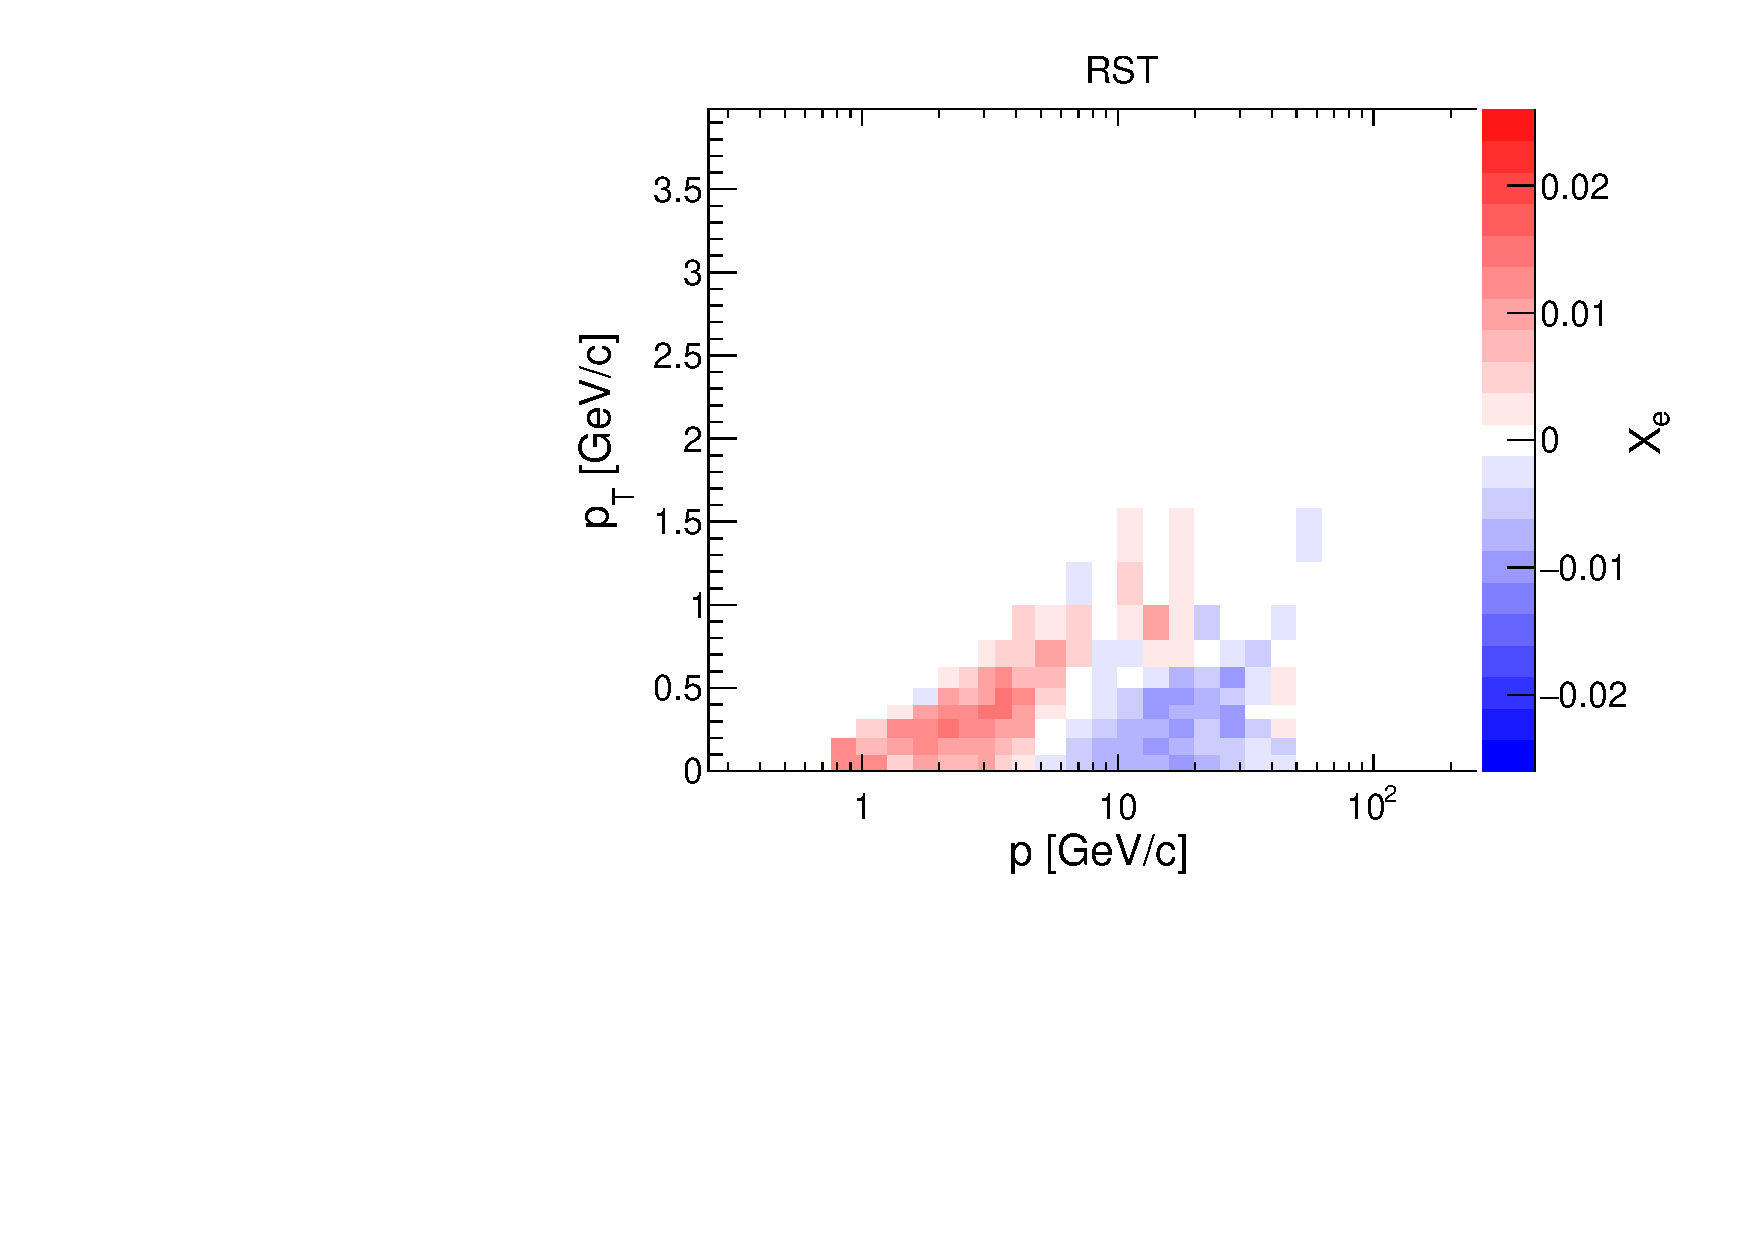
\includegraphics[clip, rviewport=0 0 1 0.94,width=0.4\textwidth]{dedx/model_158_v0_m2}
  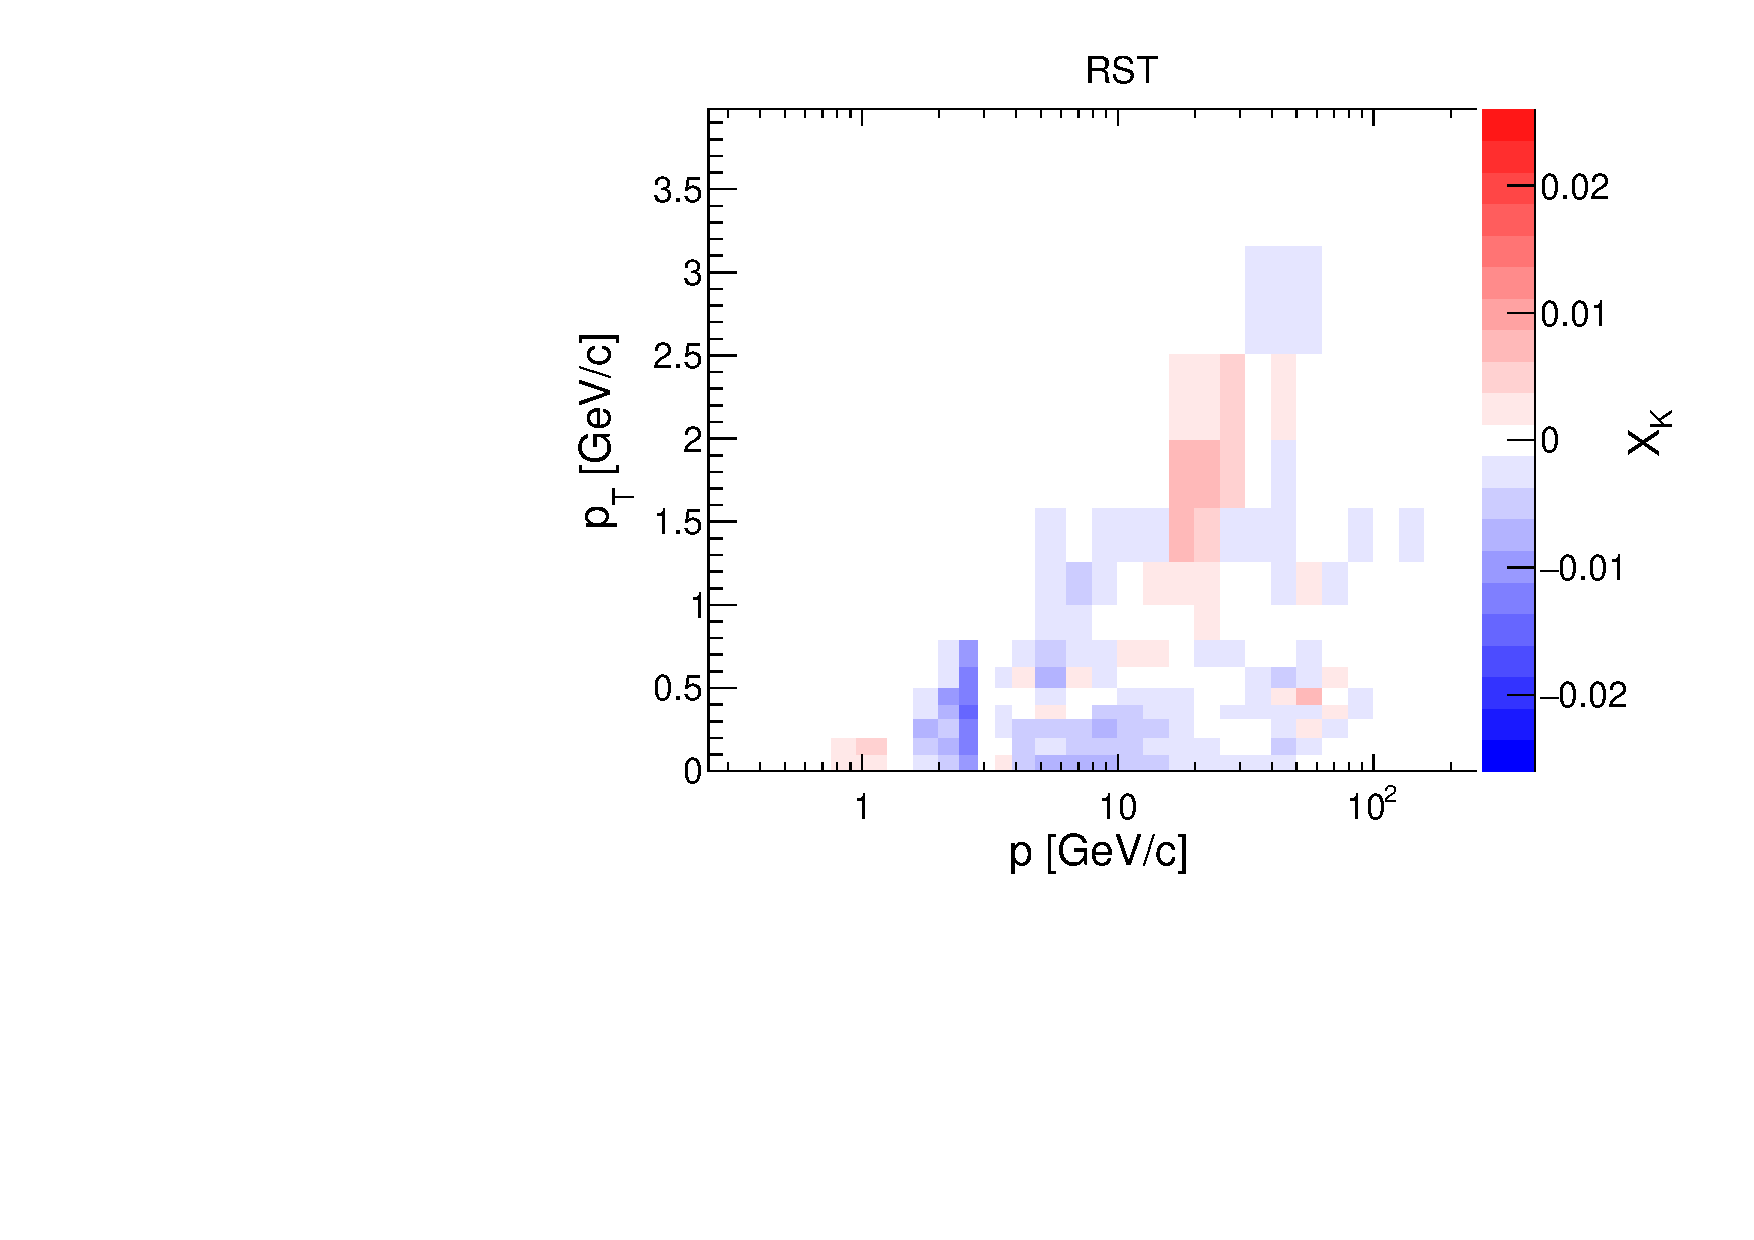
\includegraphics[clip, rviewport=0 0 1 0.94,width=0.4\textwidth]{dedx/model_158_v0_m3}

  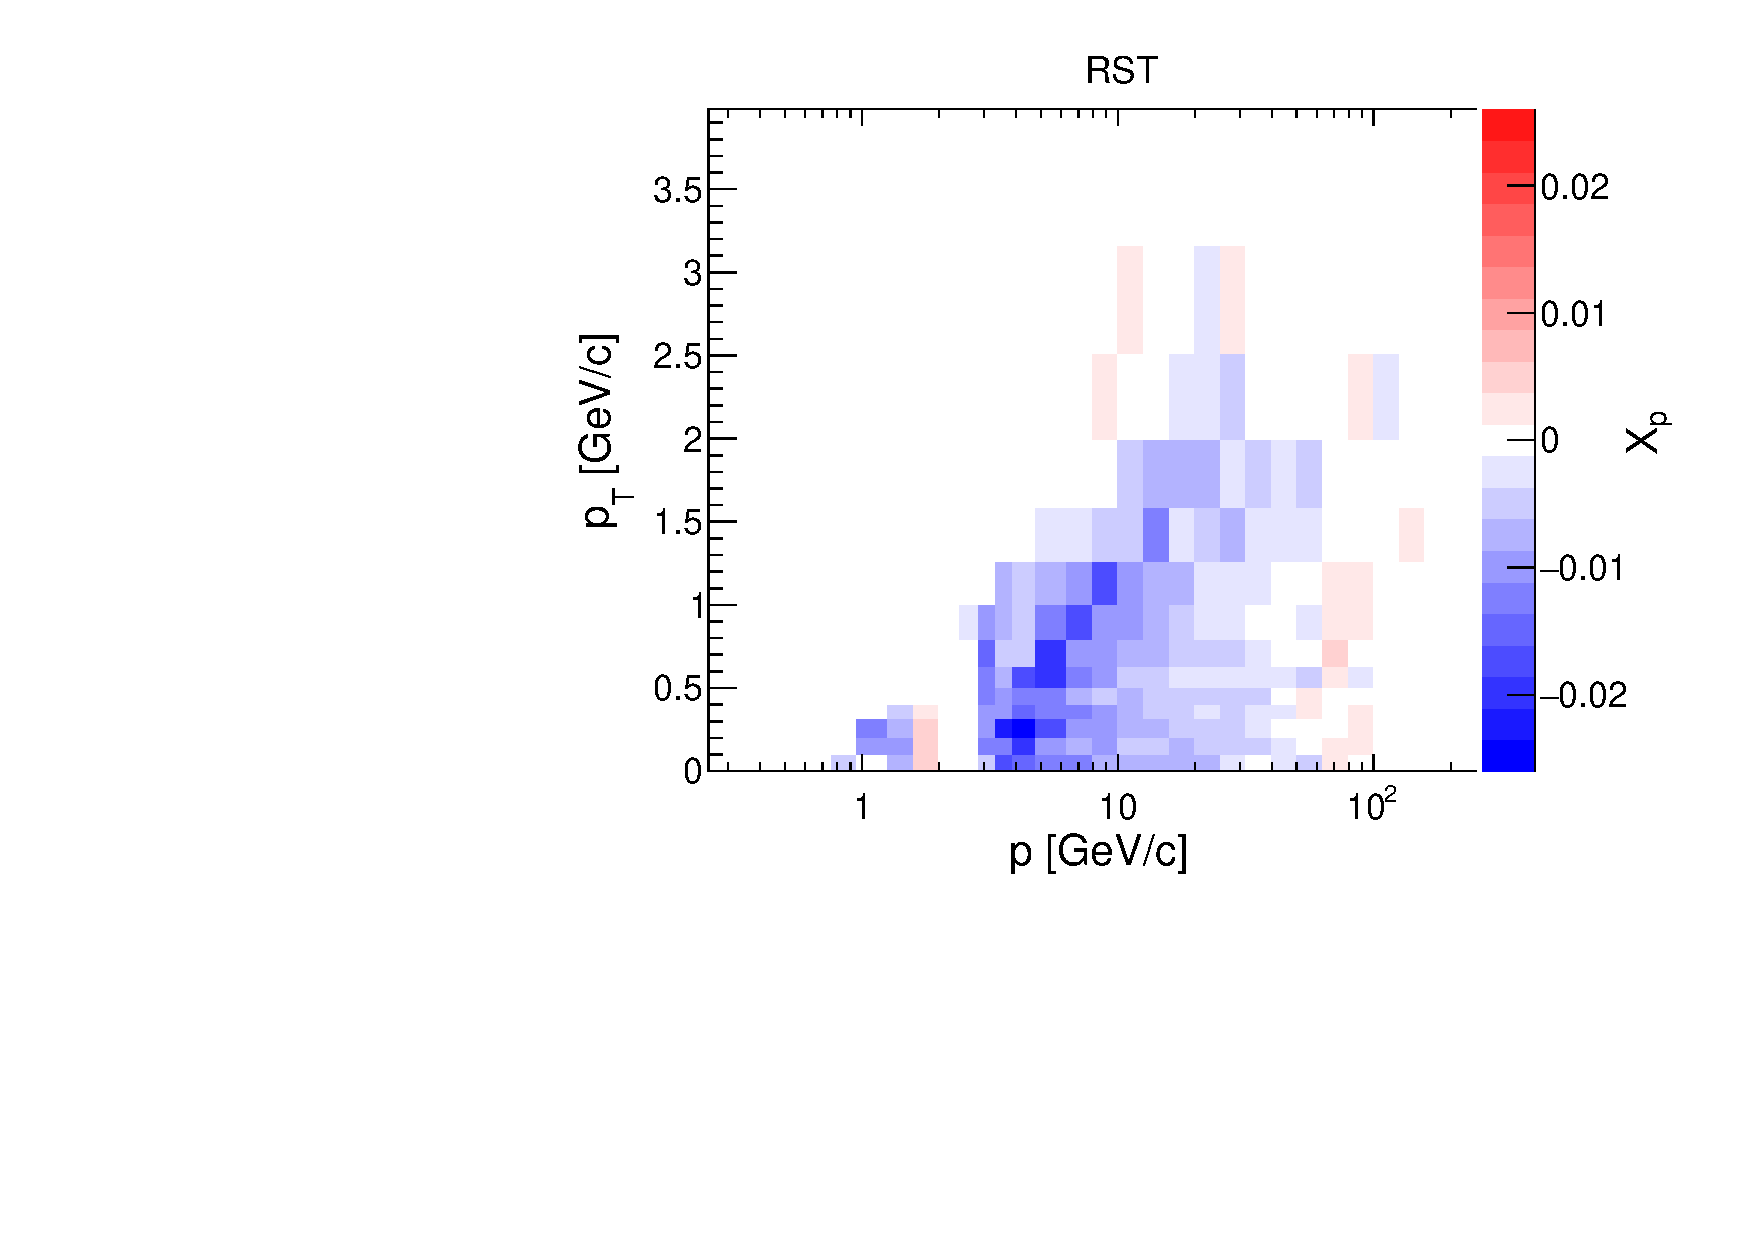
\includegraphics[clip, rviewport=0 0 1 0.94,width=0.4\textwidth]{dedx/model_158_v0_m4}
  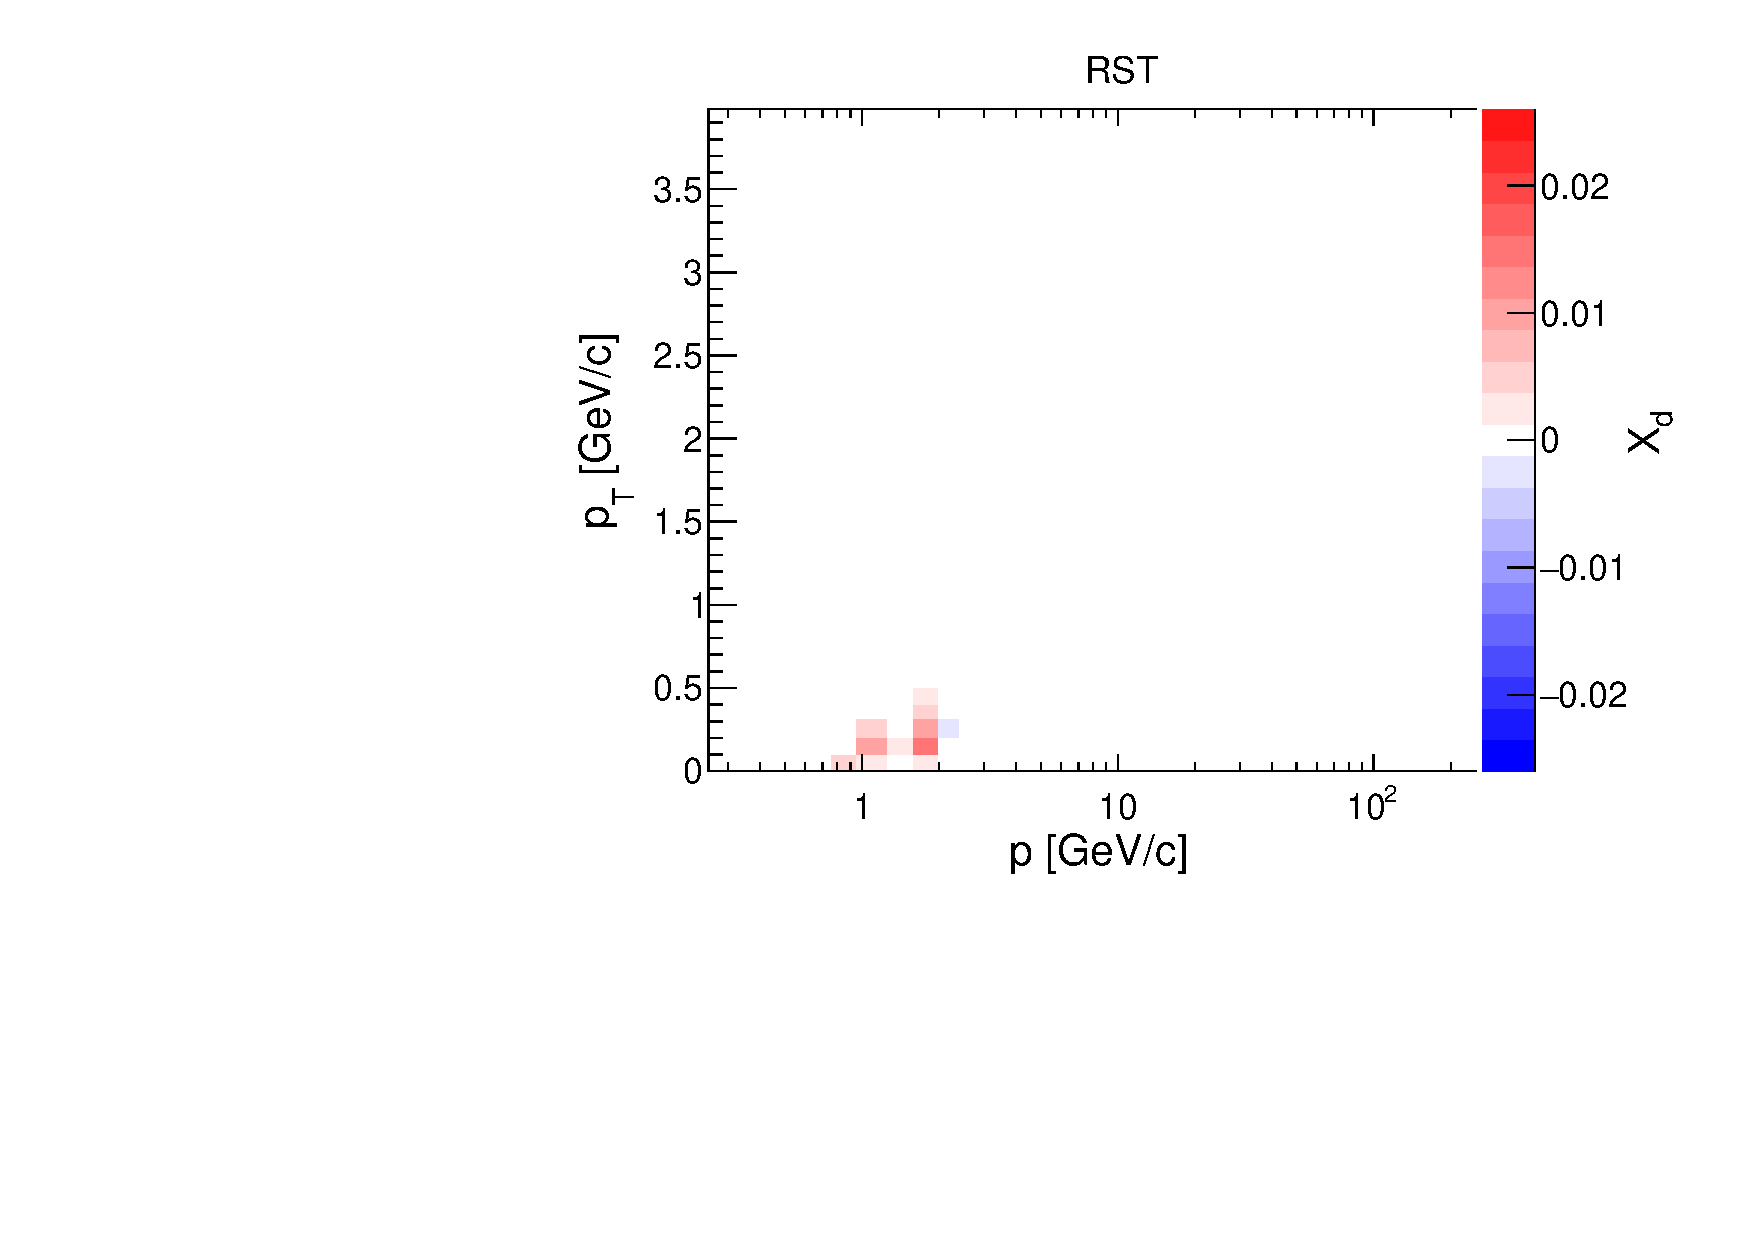
\includegraphics[clip, rviewport=0 0 1 0.94,width=0.4\textwidth]{dedx/model_158_v0_m5}
  \caption{Calibration constants obtained from the fit of the RST dataset at 158 \GeVc.}
  \label{fig:hadron:dedx:fit:cal158r}
\end{figure}


Examples of the shape parameters for the RST and 158 \GeVc dataset
are shown in~\cref{fig:hadron:dedx:fit:shape158r}. 
The remaining cases are shown
in~\cref{fig:hadron:dedx:fit:shape158w,fig:hadron:dedx:fit:shape350r,fig:hadron:dedx:fit:shape350w}. 
The parameters $\sigma_0^+$ and $\sigma_0^-$ present
only a weak phase space dependence, exhibiting values centered at
0.4, and rarely smaller than 0.35 or larger than 0.5.
Concerning the parameters $\alpha$ and $d$, a peculiar behavior
is observed: a region of mid-\pp and mid-\pT clearly
stands out from the average behavior. In this region, the asymmetry
parameter $d$ assumes negative values and the exponent $\alpha$ 
assume values smaller than the average.
Since the source of this behavior is not well understood,
a contribution to the systematic uncertainties will be estimated.
See~\cref{sec:hadron:spec:syst} for the details.

%%%%%%%%%% SHAPE %%%%%%%%%%%%%%
\begin{figure}[!ht]
  \centering
  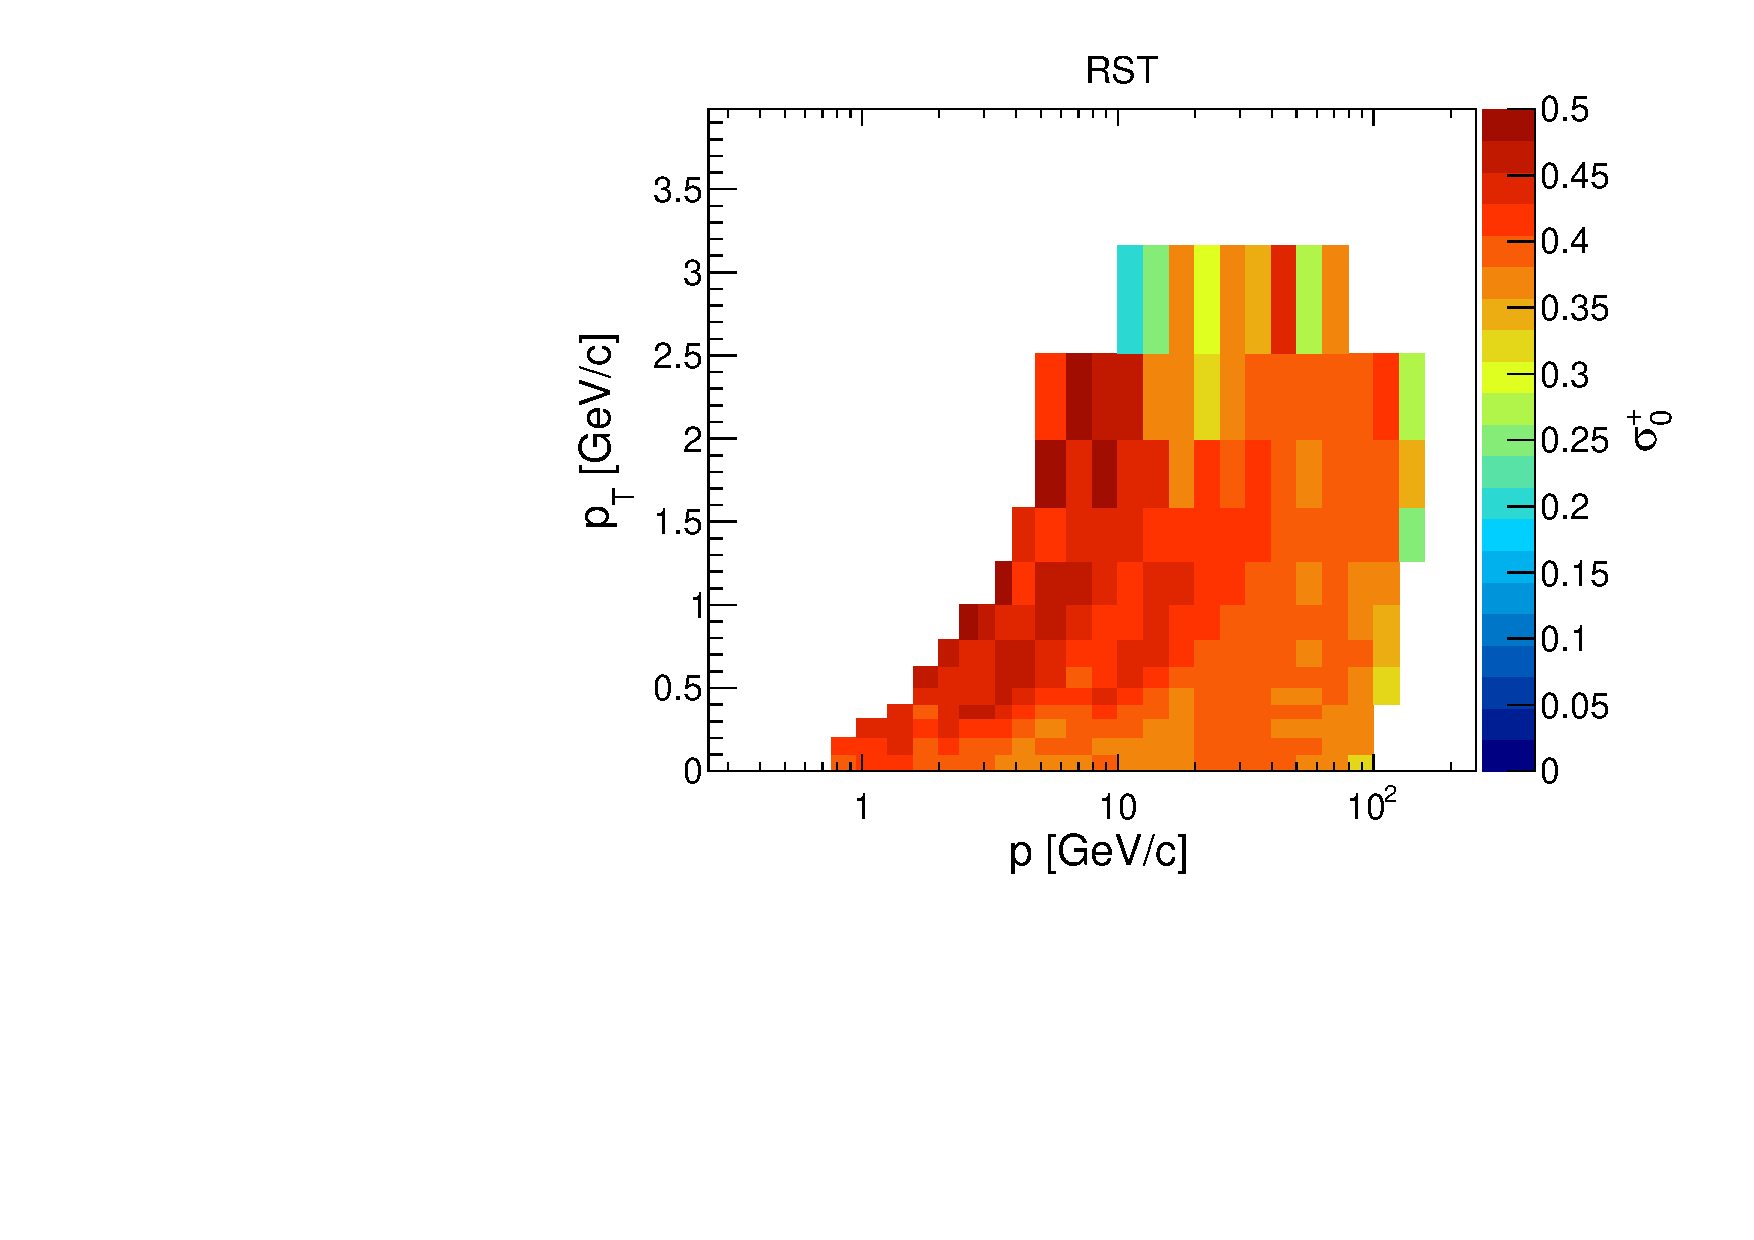
\includegraphics[clip, rviewport=0 0 1 0.94,width=0.4\textwidth]{dedx/model_158_v0_m6}
  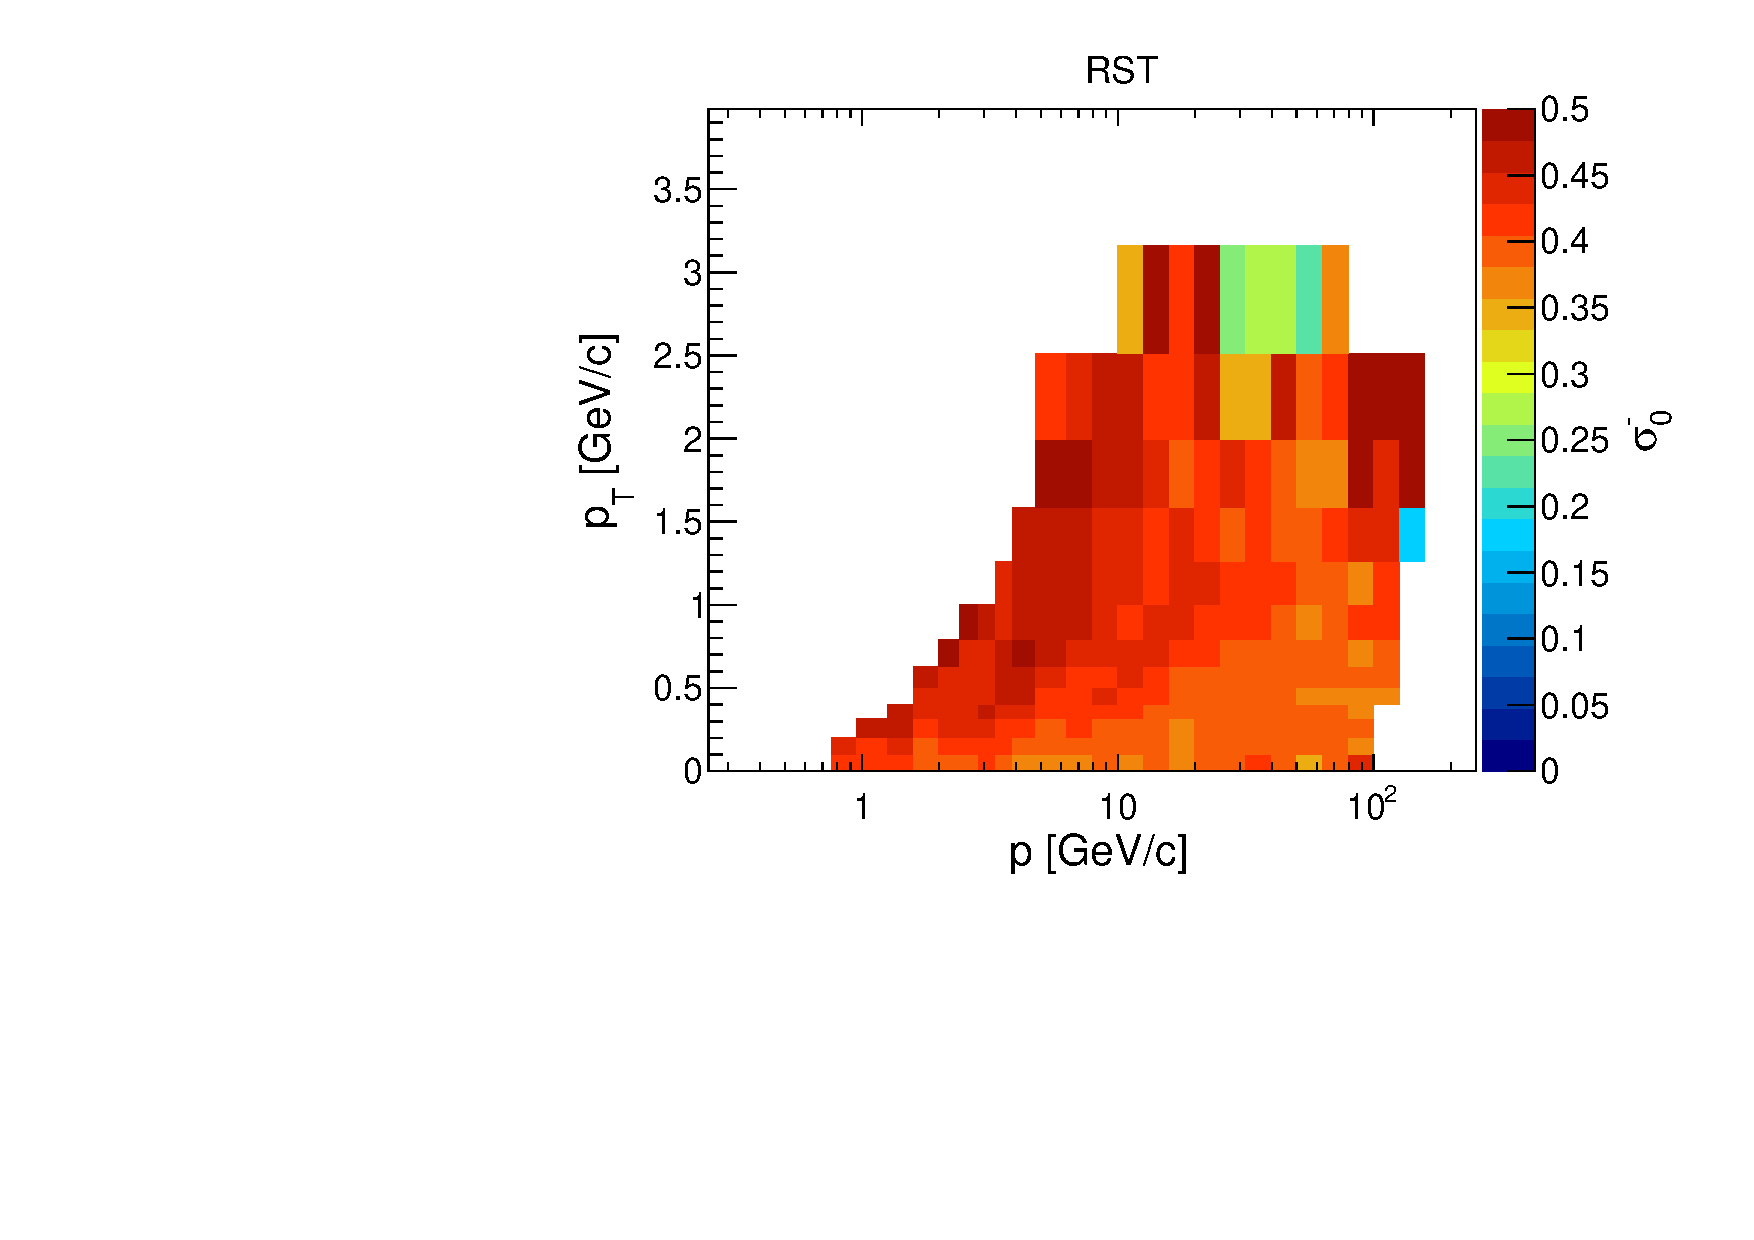
\includegraphics[clip, rviewport=0 0 1 0.94,width=0.4\textwidth]{dedx/model_158_v0_m7}

  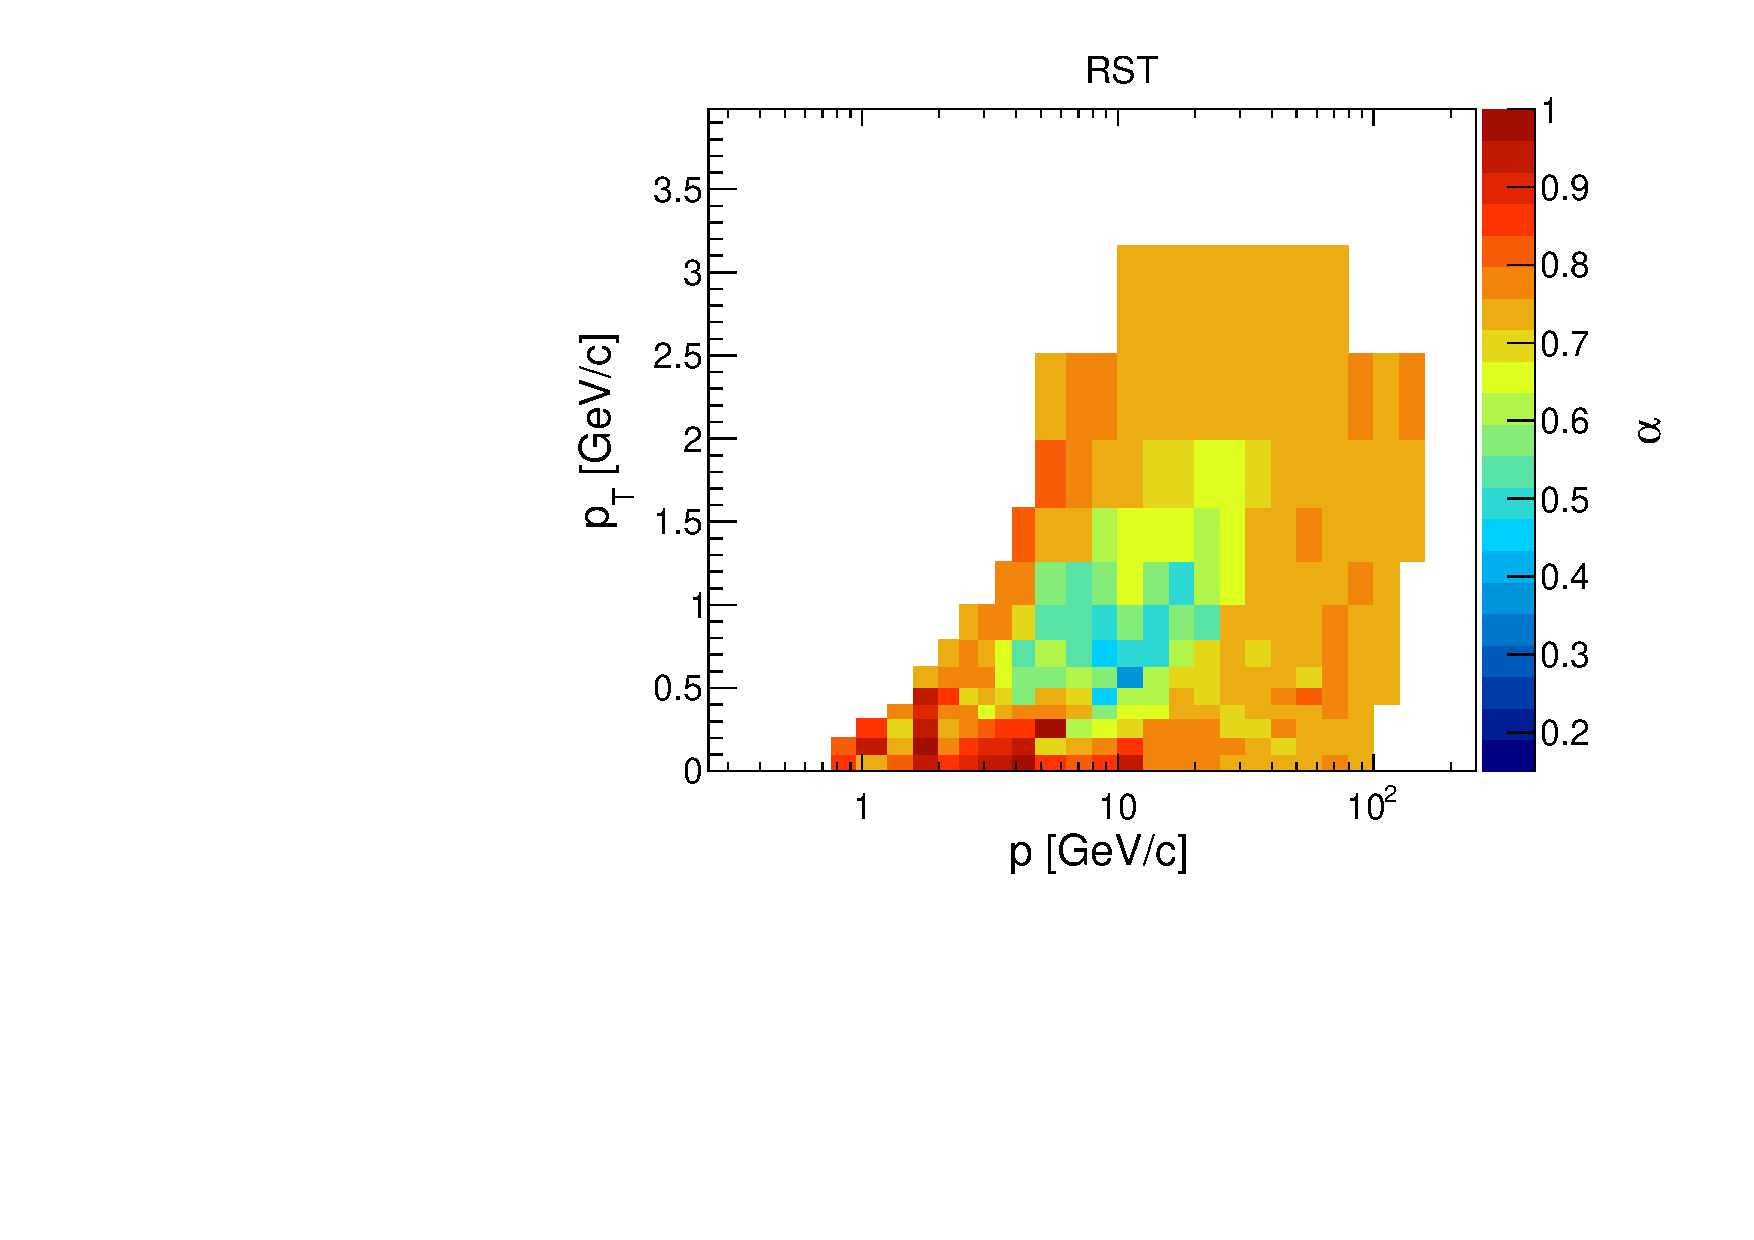
\includegraphics[clip, rviewport=0 0 1 0.94,width=0.4\textwidth]{dedx/model_158_v0_m9}
  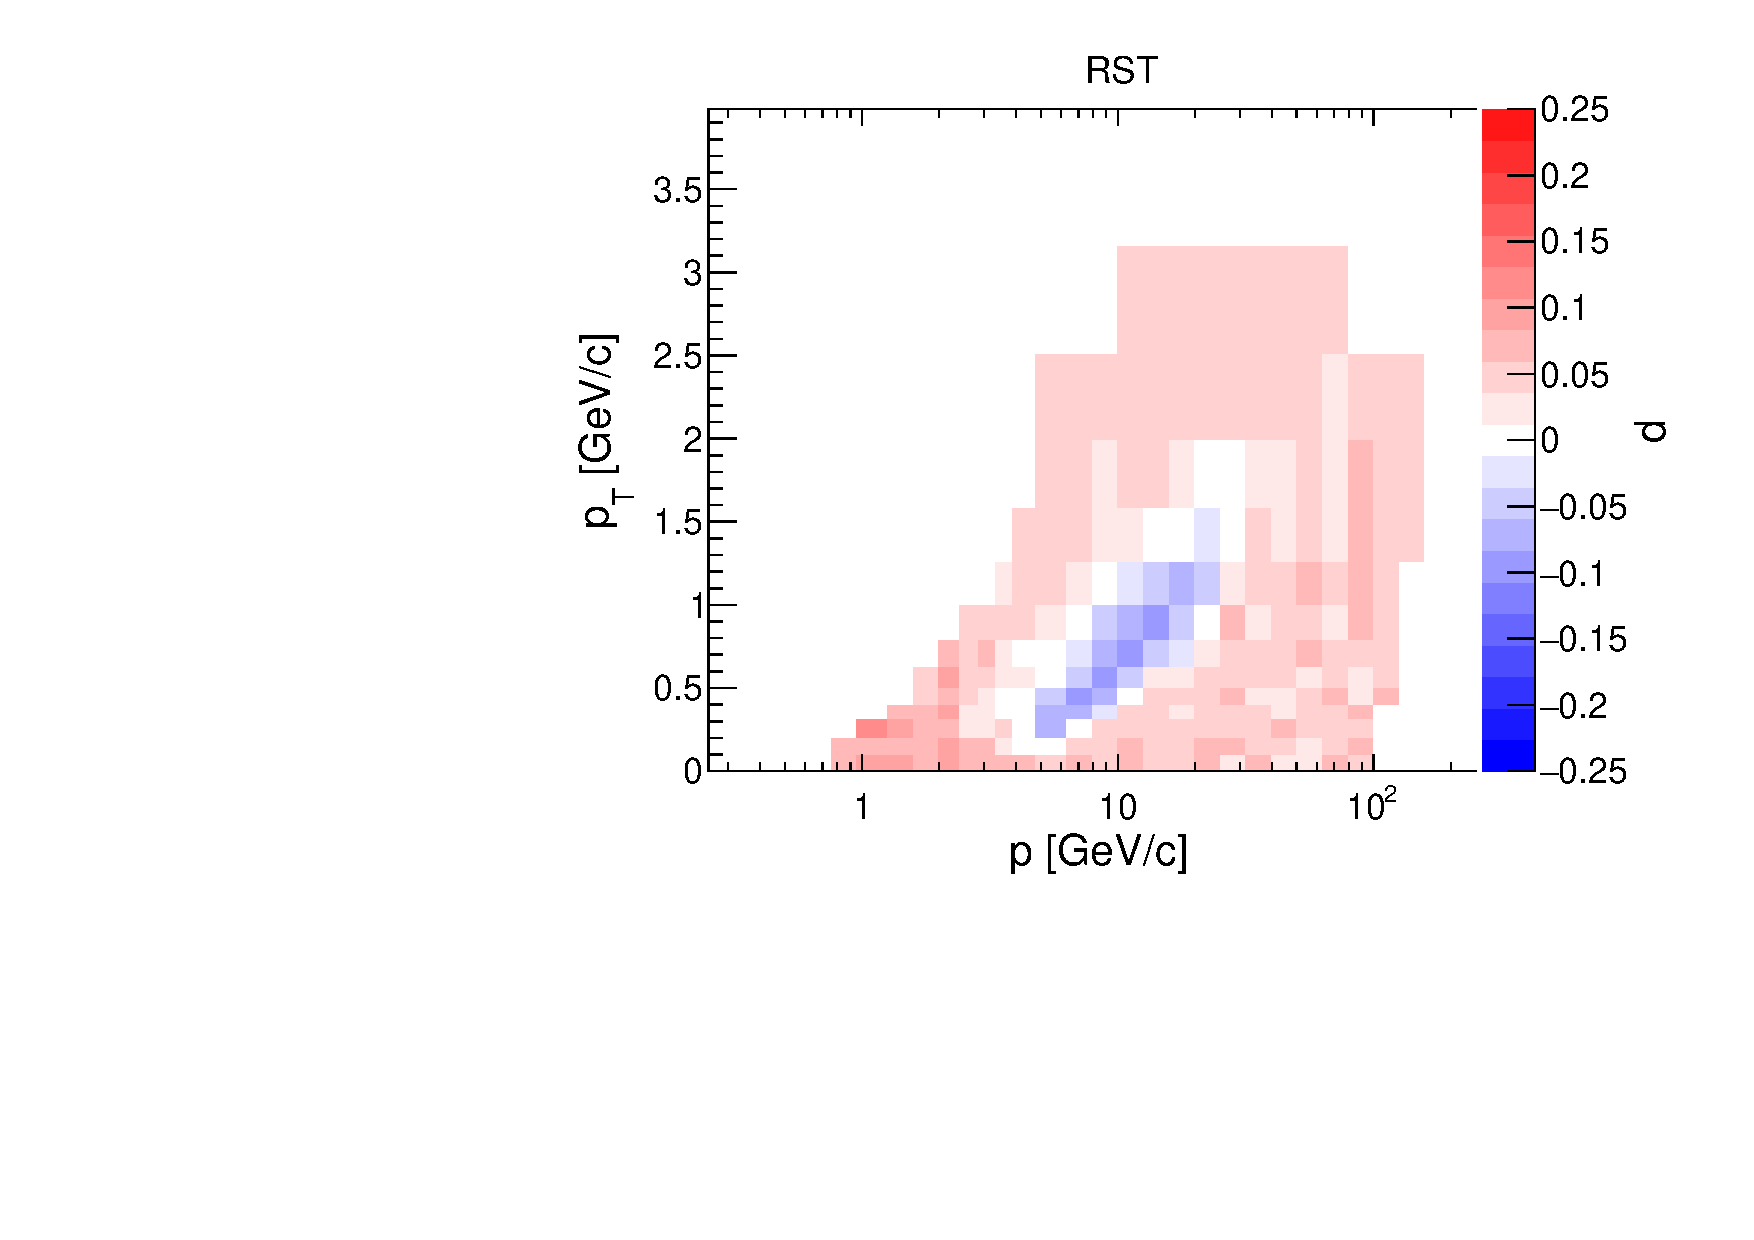
\includegraphics[clip, rviewport=0 0 1 0.94,width=0.4\textwidth]{dedx/model_158_v0_m10}
  \caption{Shape parameters obtained from the fit of the RST dataset at 158 \GeVc.}
  \label{fig:hadron:dedx:fit:shape158r}
\end{figure}

Examples of the particle fractions for RST and 158 \GeVc
with target inserted
are shown in~\cref{fig:hadron:dedx:fit:frac158r}.
The remaining cases are shown
in~\cref{fig:hadron:dedx:fit:frac158w,fig:hadron:dedx:fit:frac350r,fig:hadron:dedx:fit:frac350w}.
The fractions from the target removed dataset are shown in~\cref{sec:hadron:dedx:results}.


%%%%%%%%%% FRACTIONS %%%%%%%%%%%%%%
\begin{figure}
  \centering
  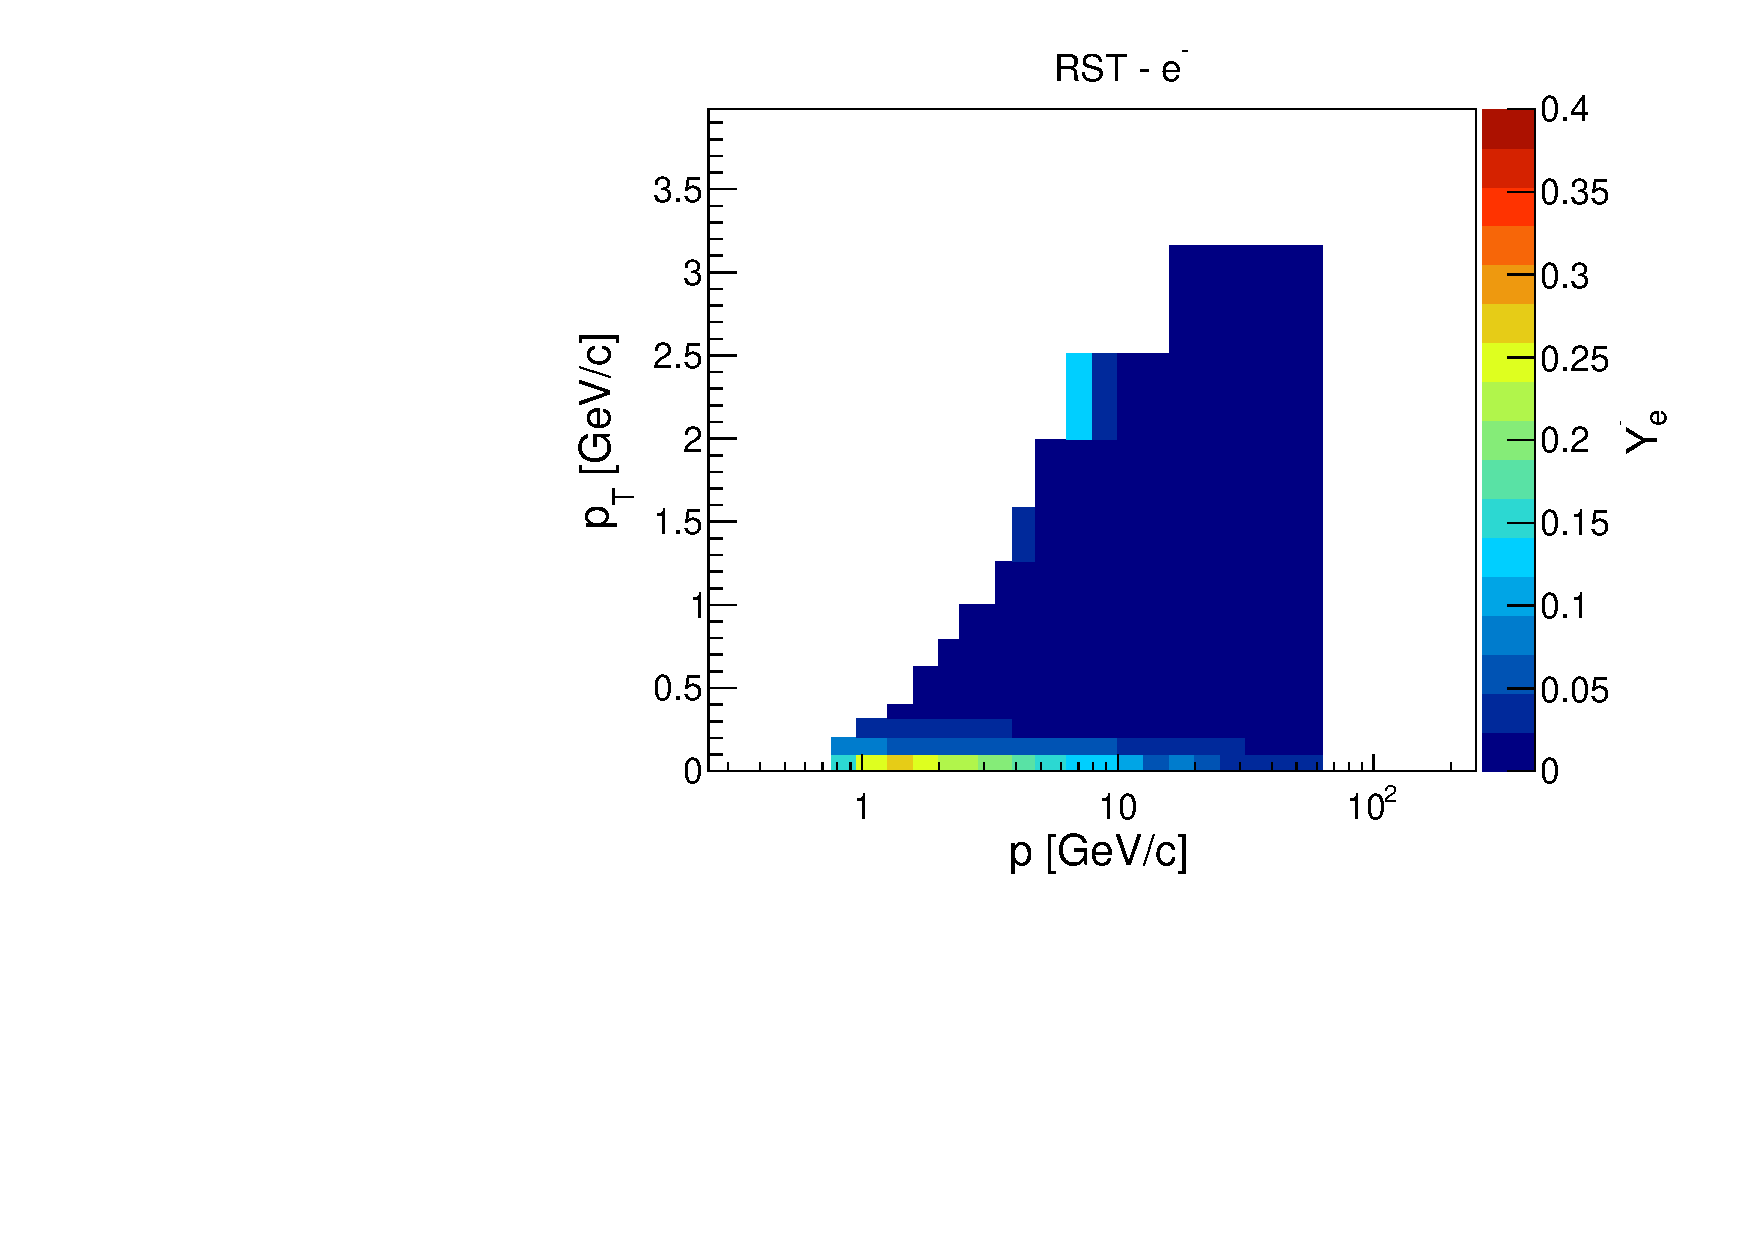
\includegraphics[clip, rviewport=0 0.13 1 0.94,width=0.4\textwidth]{dedx/fraction_158_fl0_v0_c0_p0}
  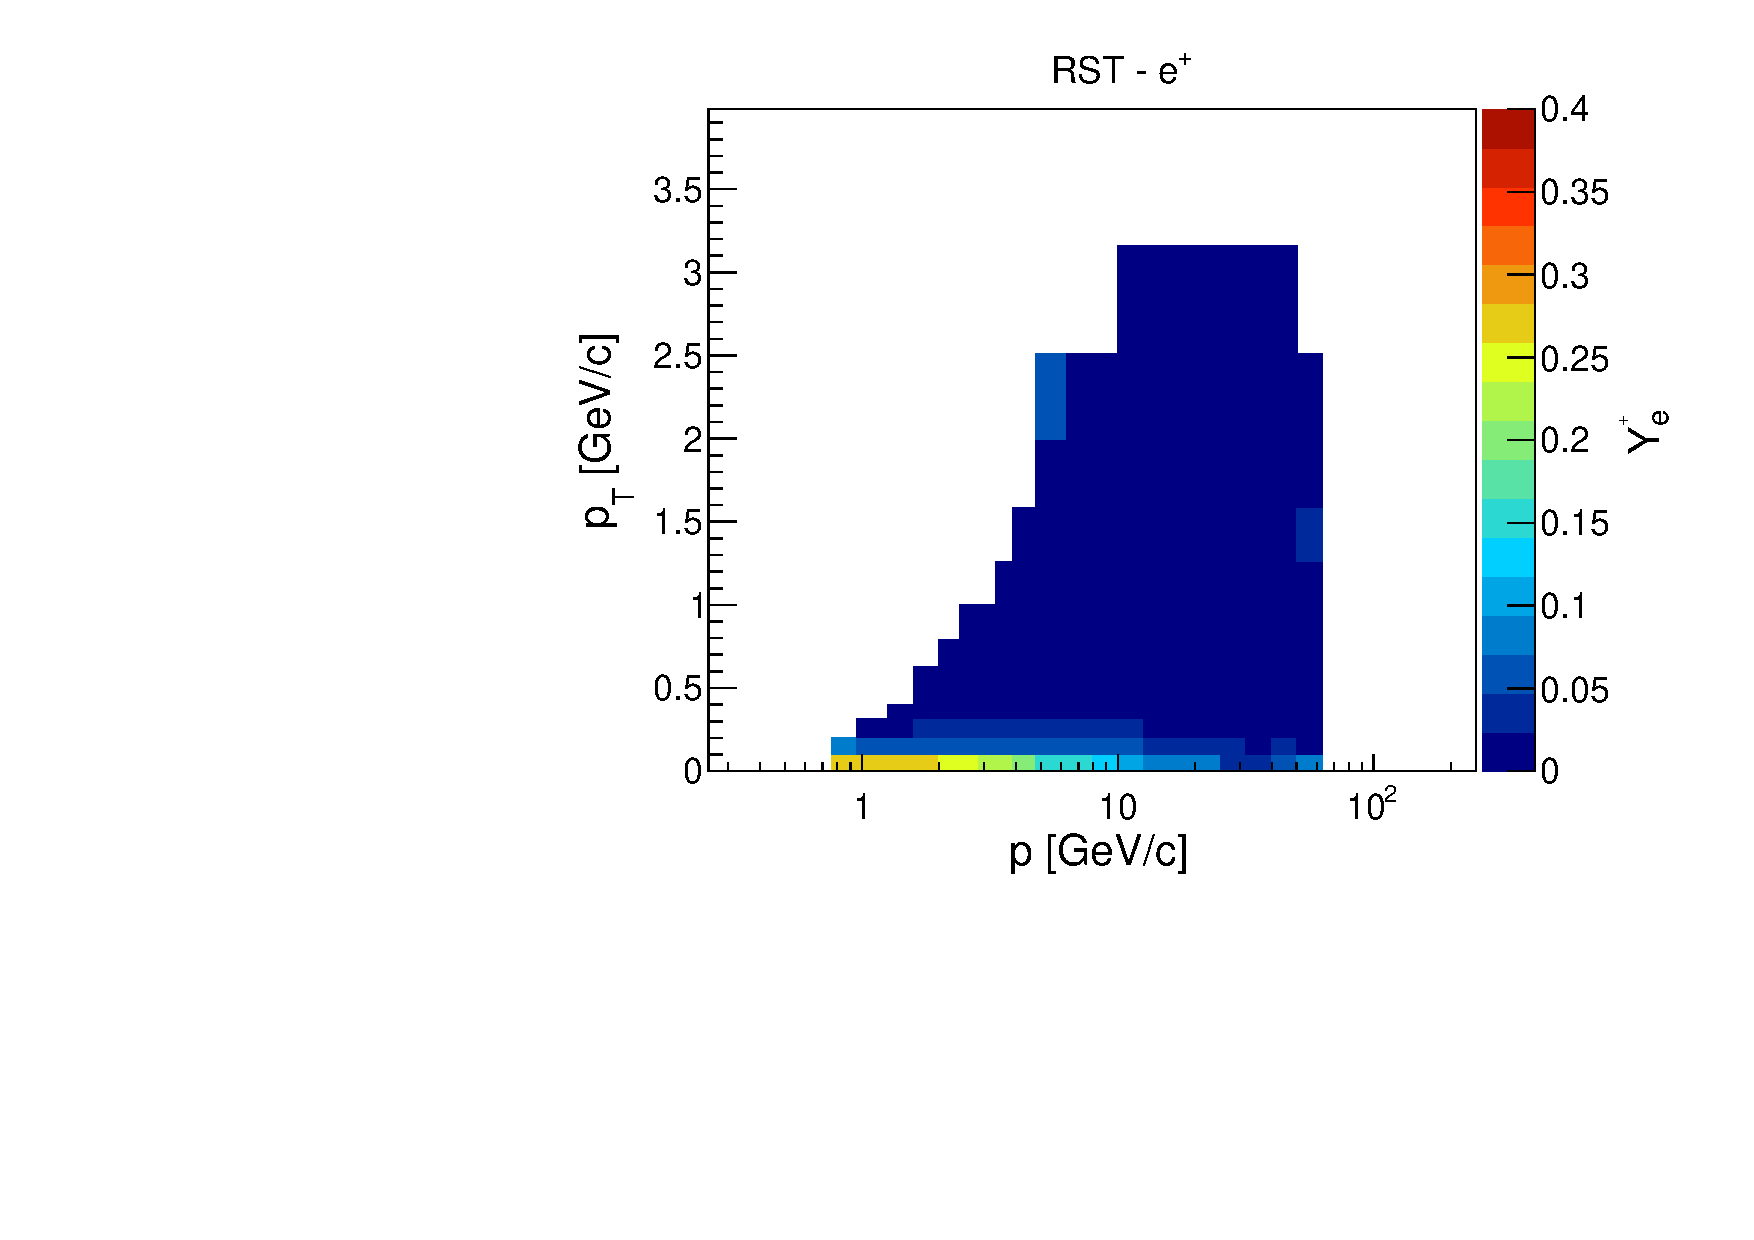
\includegraphics[clip, rviewport=0 0.13 1 0.94,width=0.4\textwidth]{dedx/fraction_158_fl0_v0_c1_p0}

  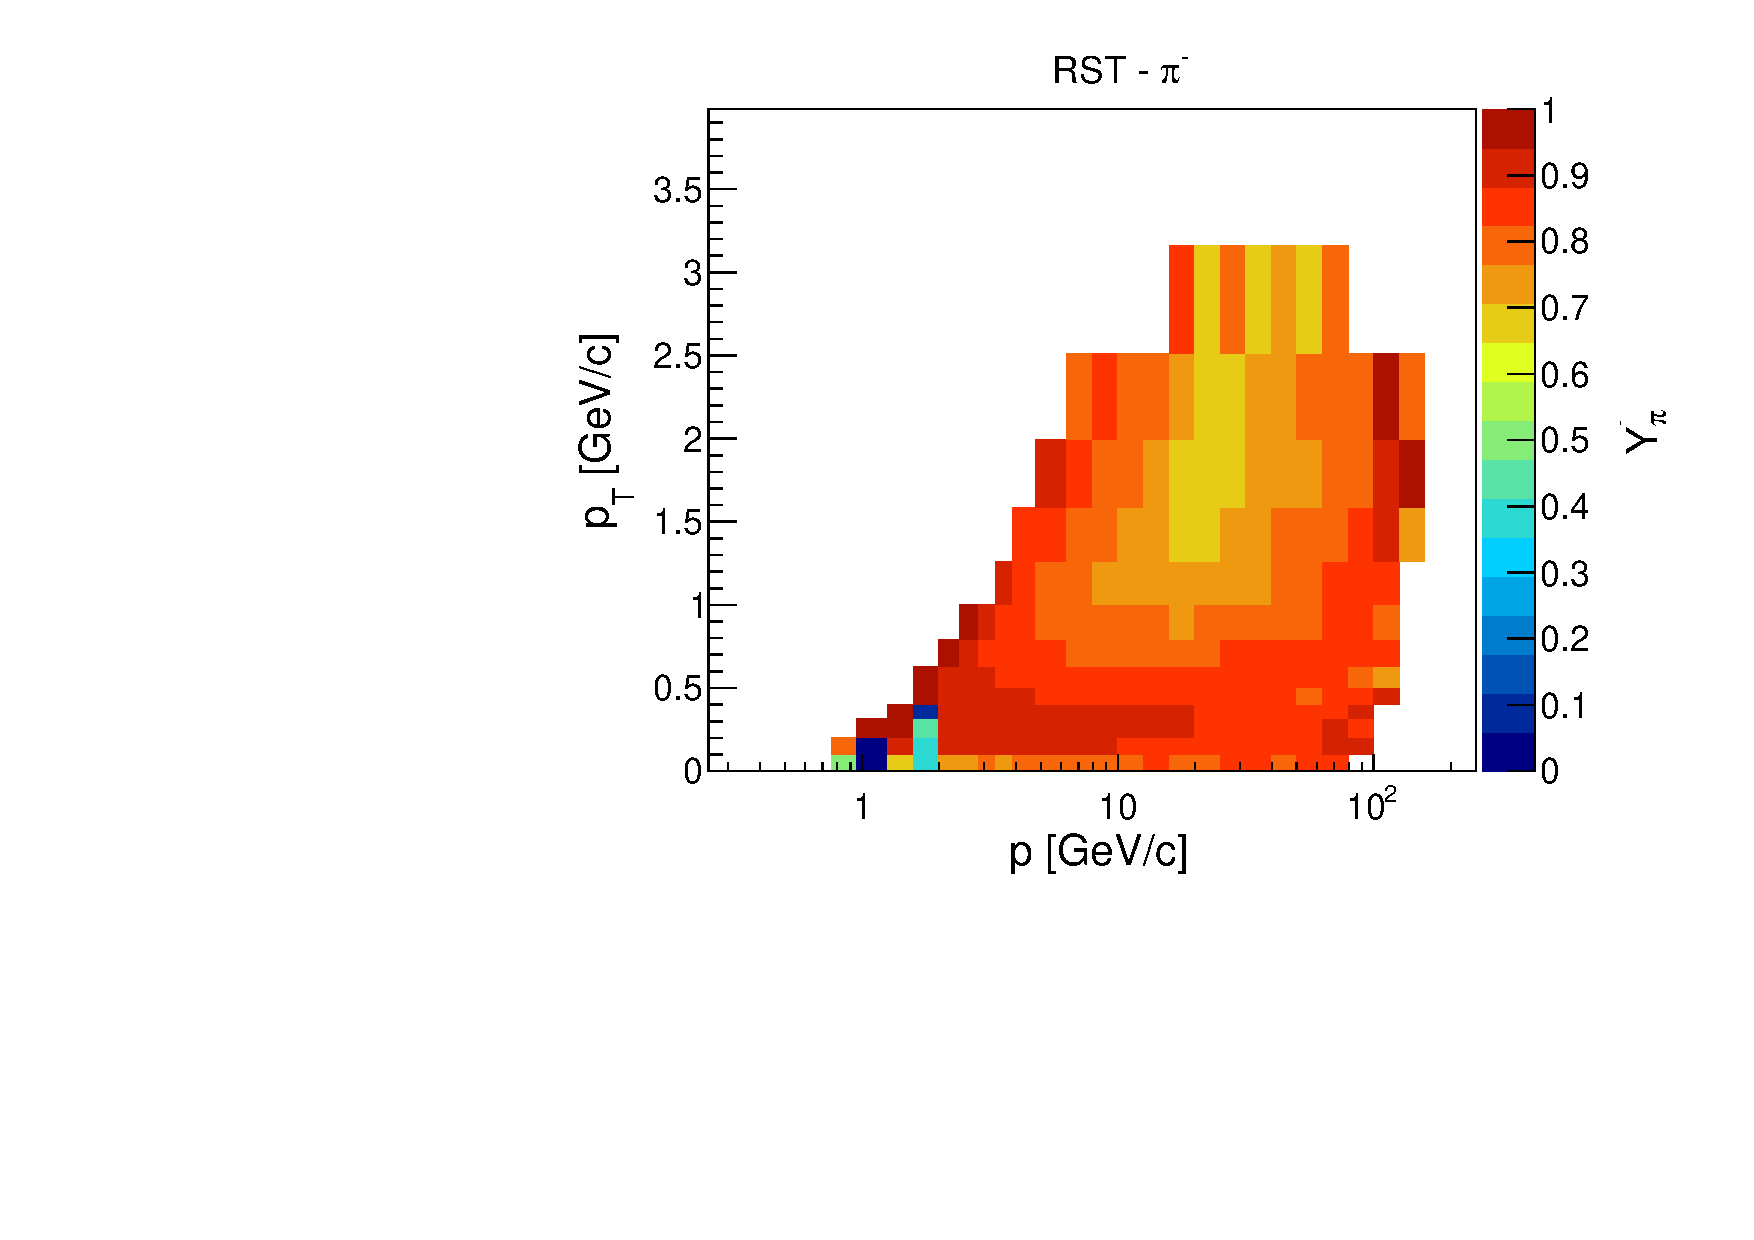
\includegraphics[clip, rviewport=0 0.13 1 0.94,width=0.4\textwidth]{dedx/fraction_158_fl0_v0_c0_p1}
  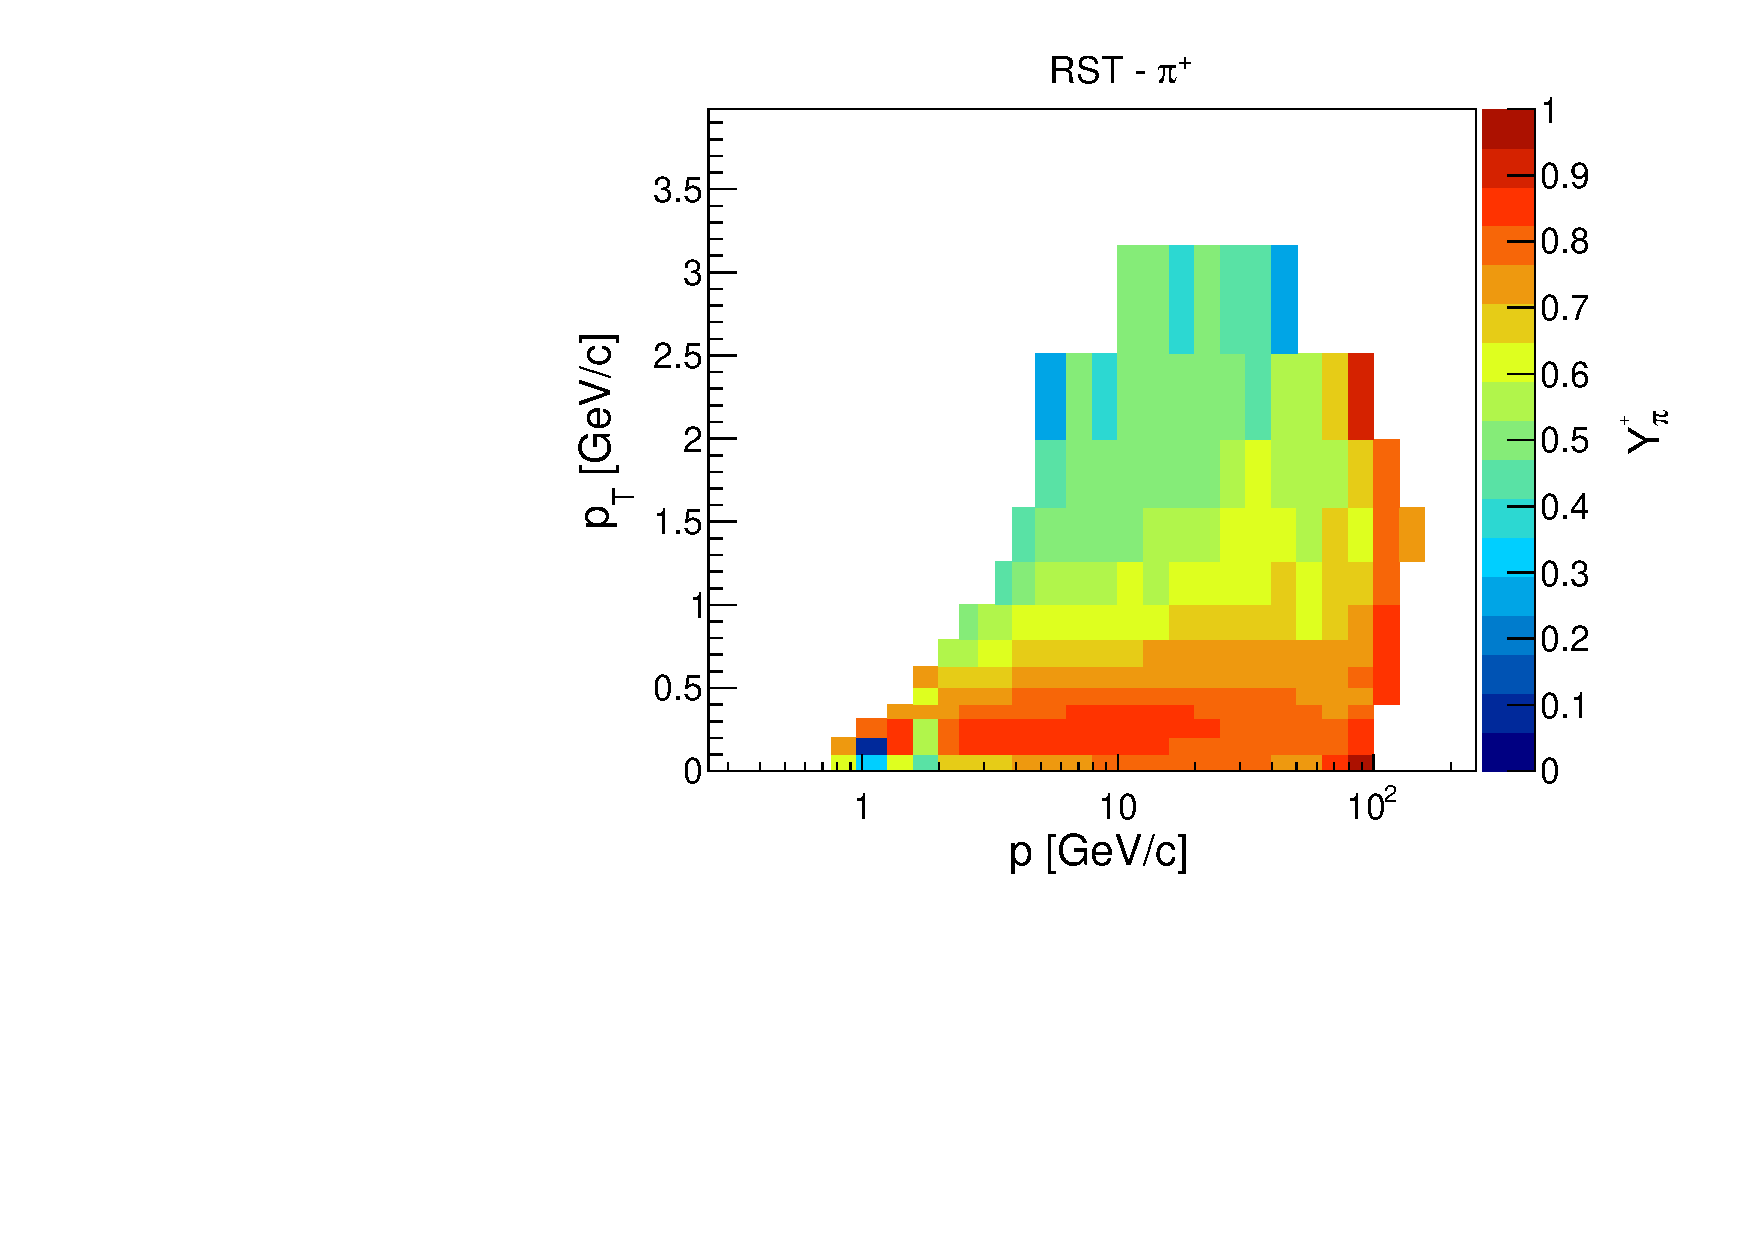
\includegraphics[clip, rviewport=0 0.13 1 0.94,width=0.4\textwidth]{dedx/fraction_158_fl0_v0_c1_p1}

  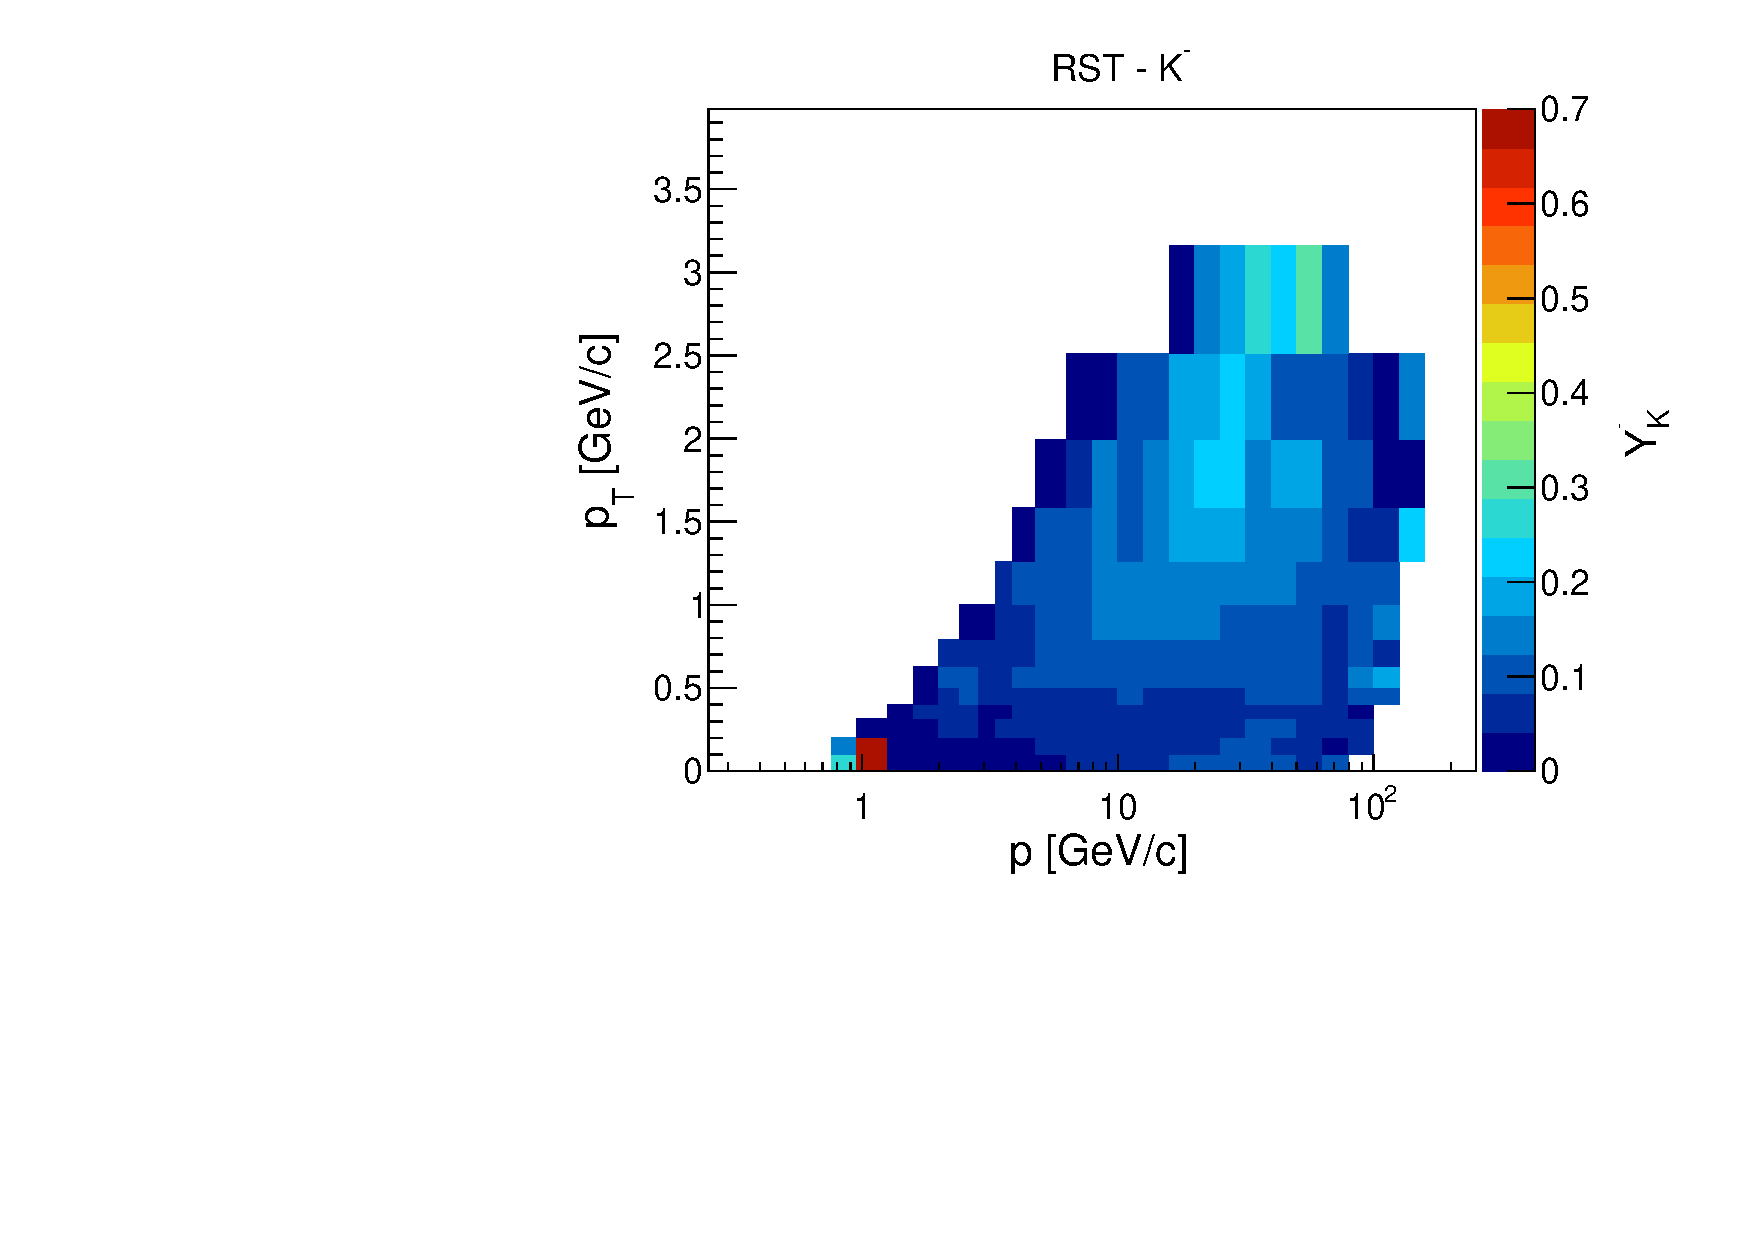
\includegraphics[clip, rviewport=0 0.13 1 0.94,width=0.4\textwidth]{dedx/fraction_158_fl0_v0_c0_p2}
  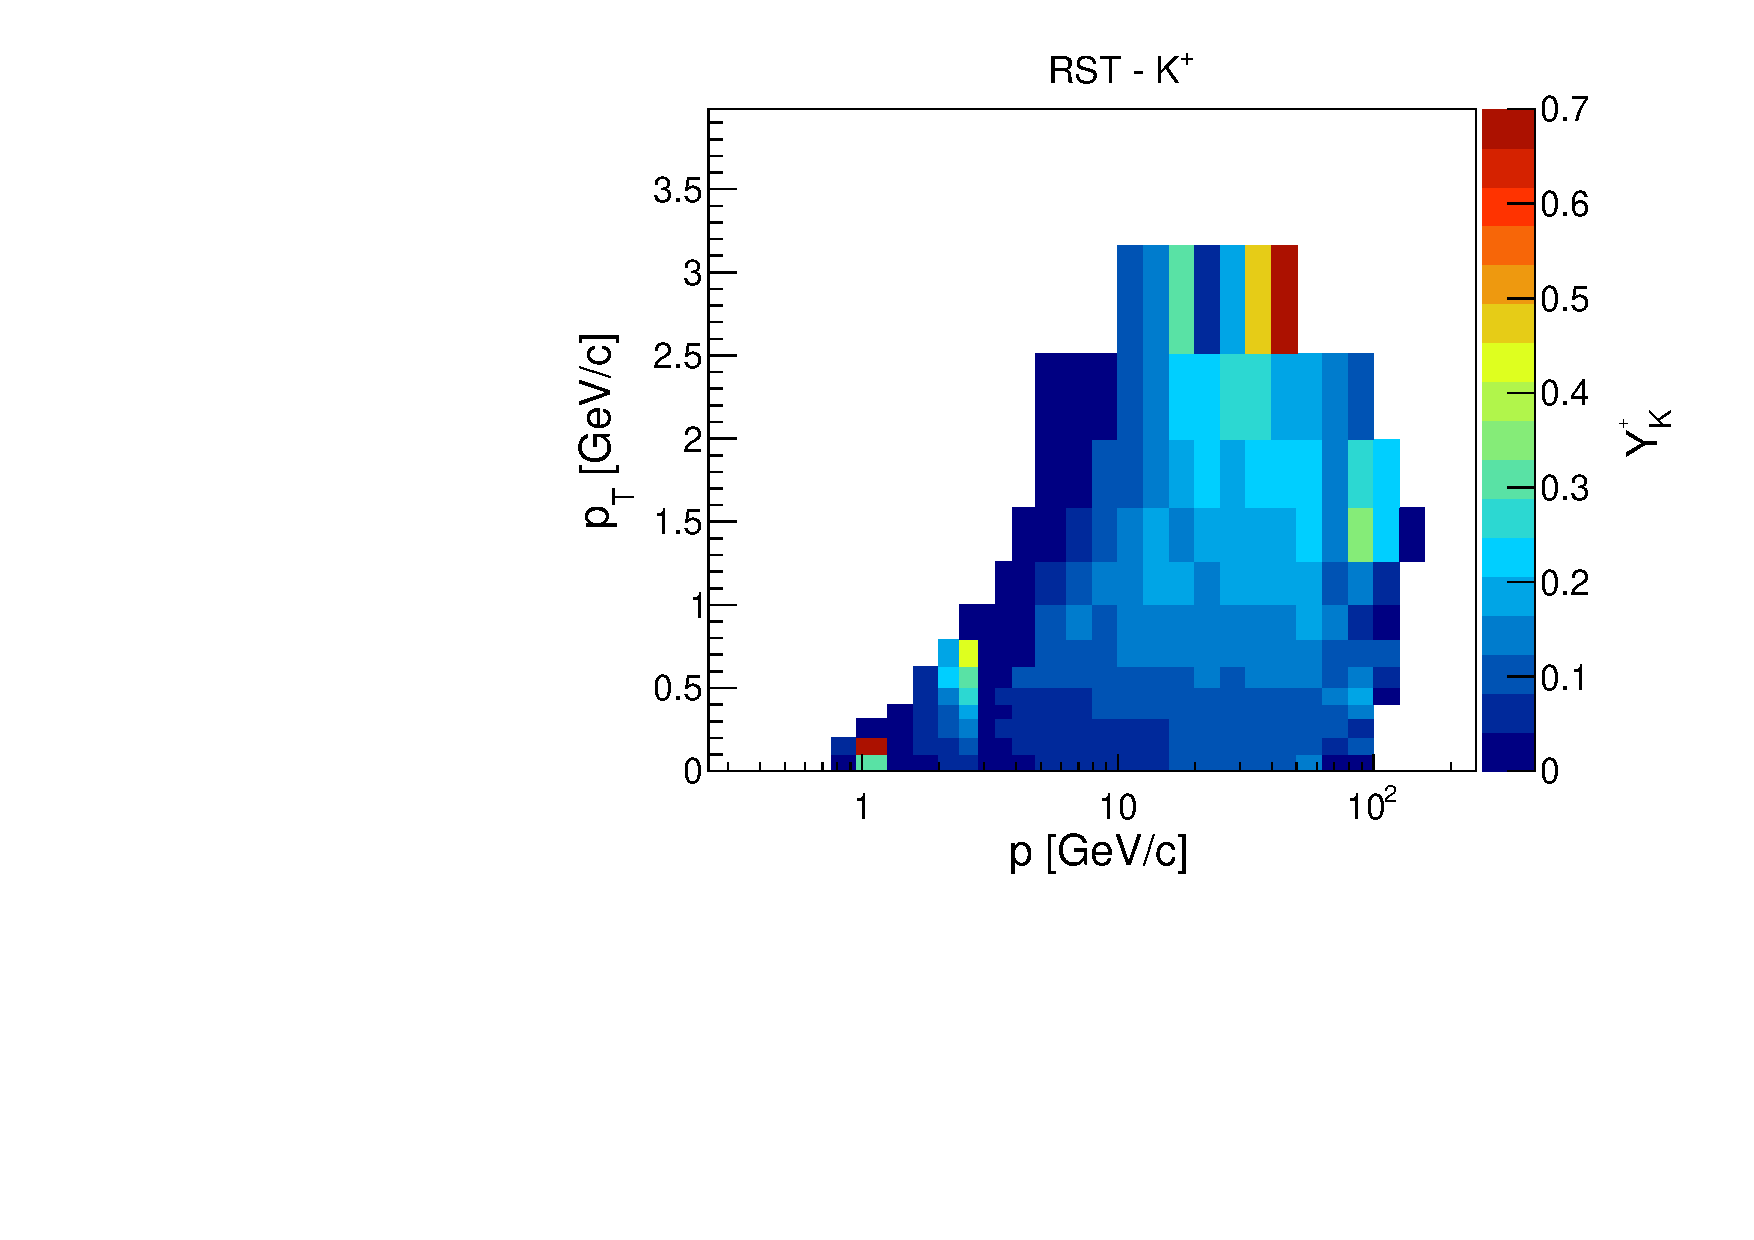
\includegraphics[clip, rviewport=0 0.13 1 0.94,width=0.4\textwidth]{dedx/fraction_158_fl0_v0_c1_p2}


  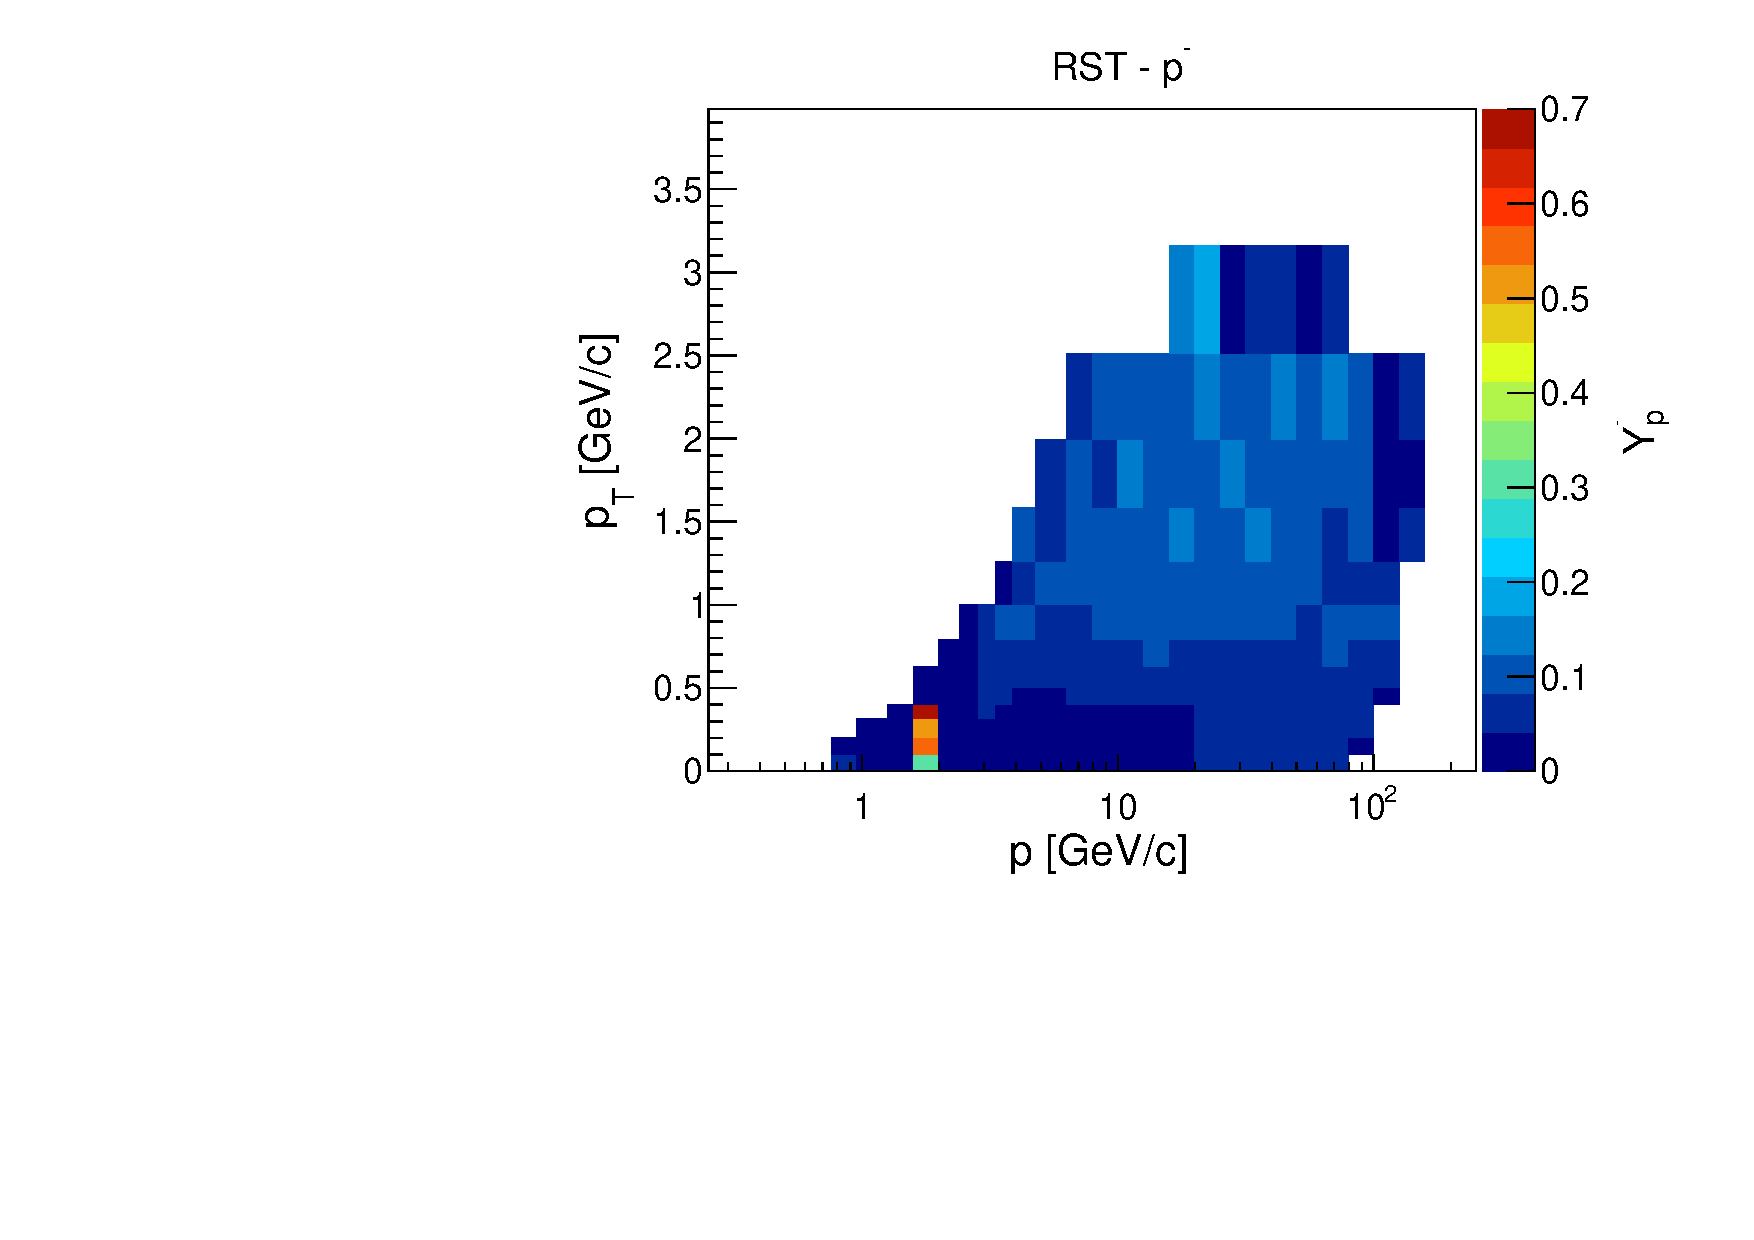
\includegraphics[clip, rviewport=0 0.13 1 0.94,width=0.4\textwidth]{dedx/fraction_158_fl0_v0_c0_p3}
  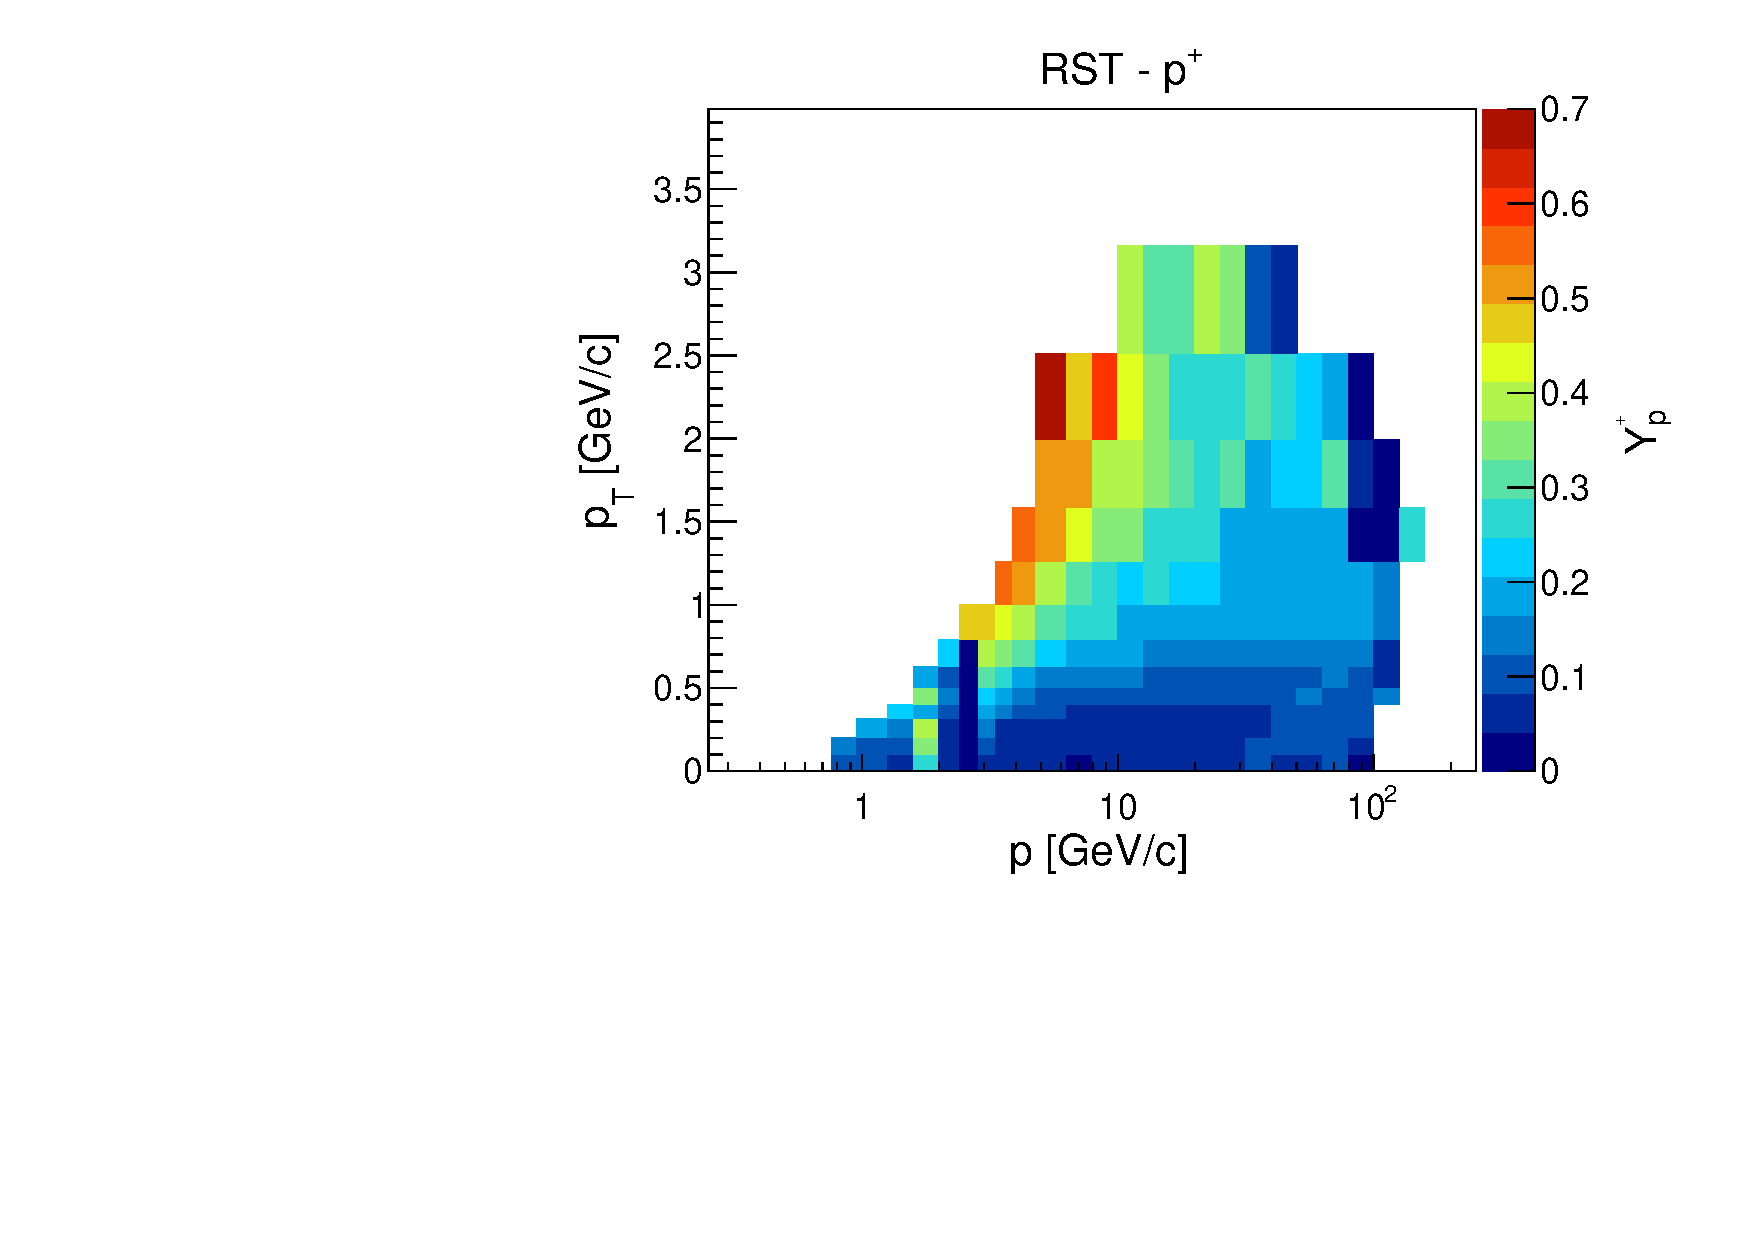
\includegraphics[clip, rviewport=0 0.13 1 0.94,width=0.4\textwidth]{dedx/fraction_158_fl0_v0_c1_p3}

  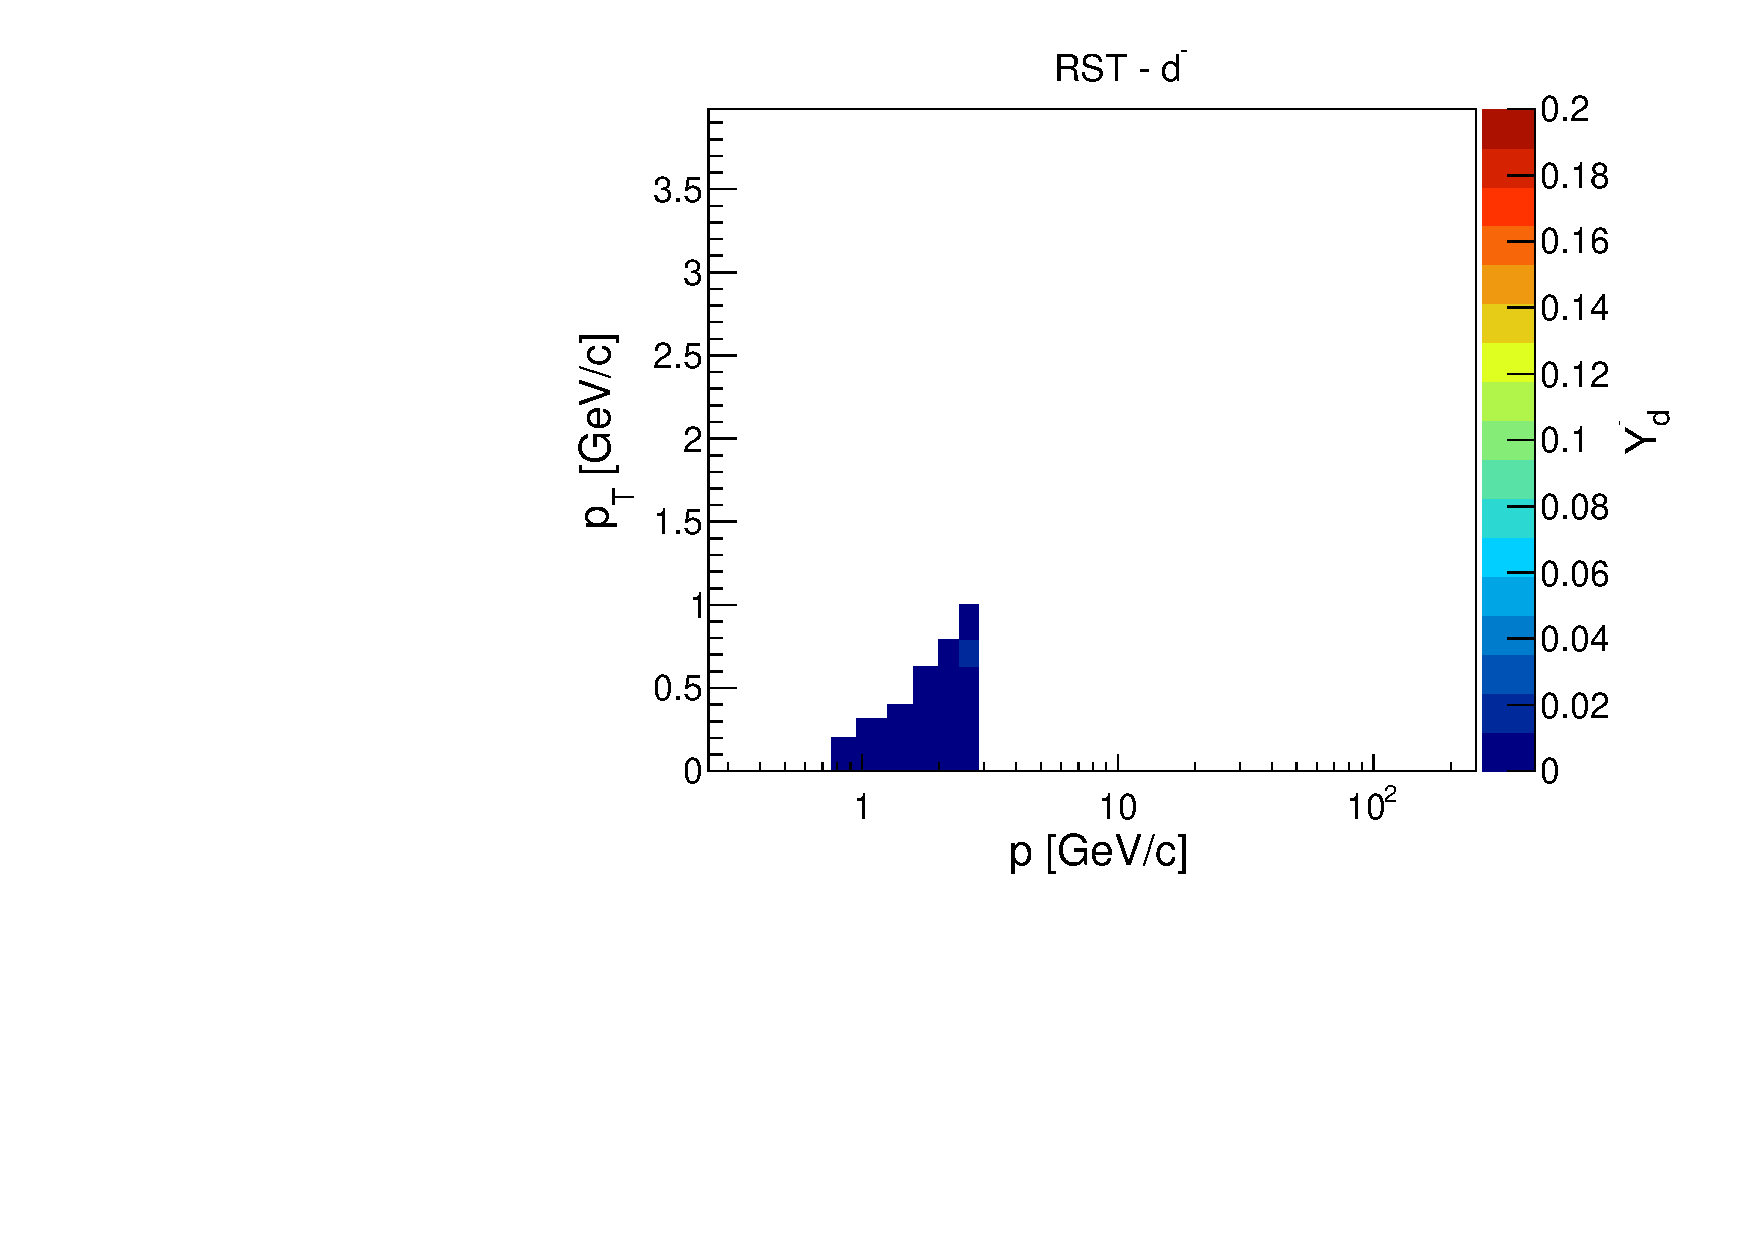
\includegraphics[clip, rviewport=0 0 1 0.94,width=0.4\textwidth]{dedx/fraction_158_fl0_v0_c0_p4}
  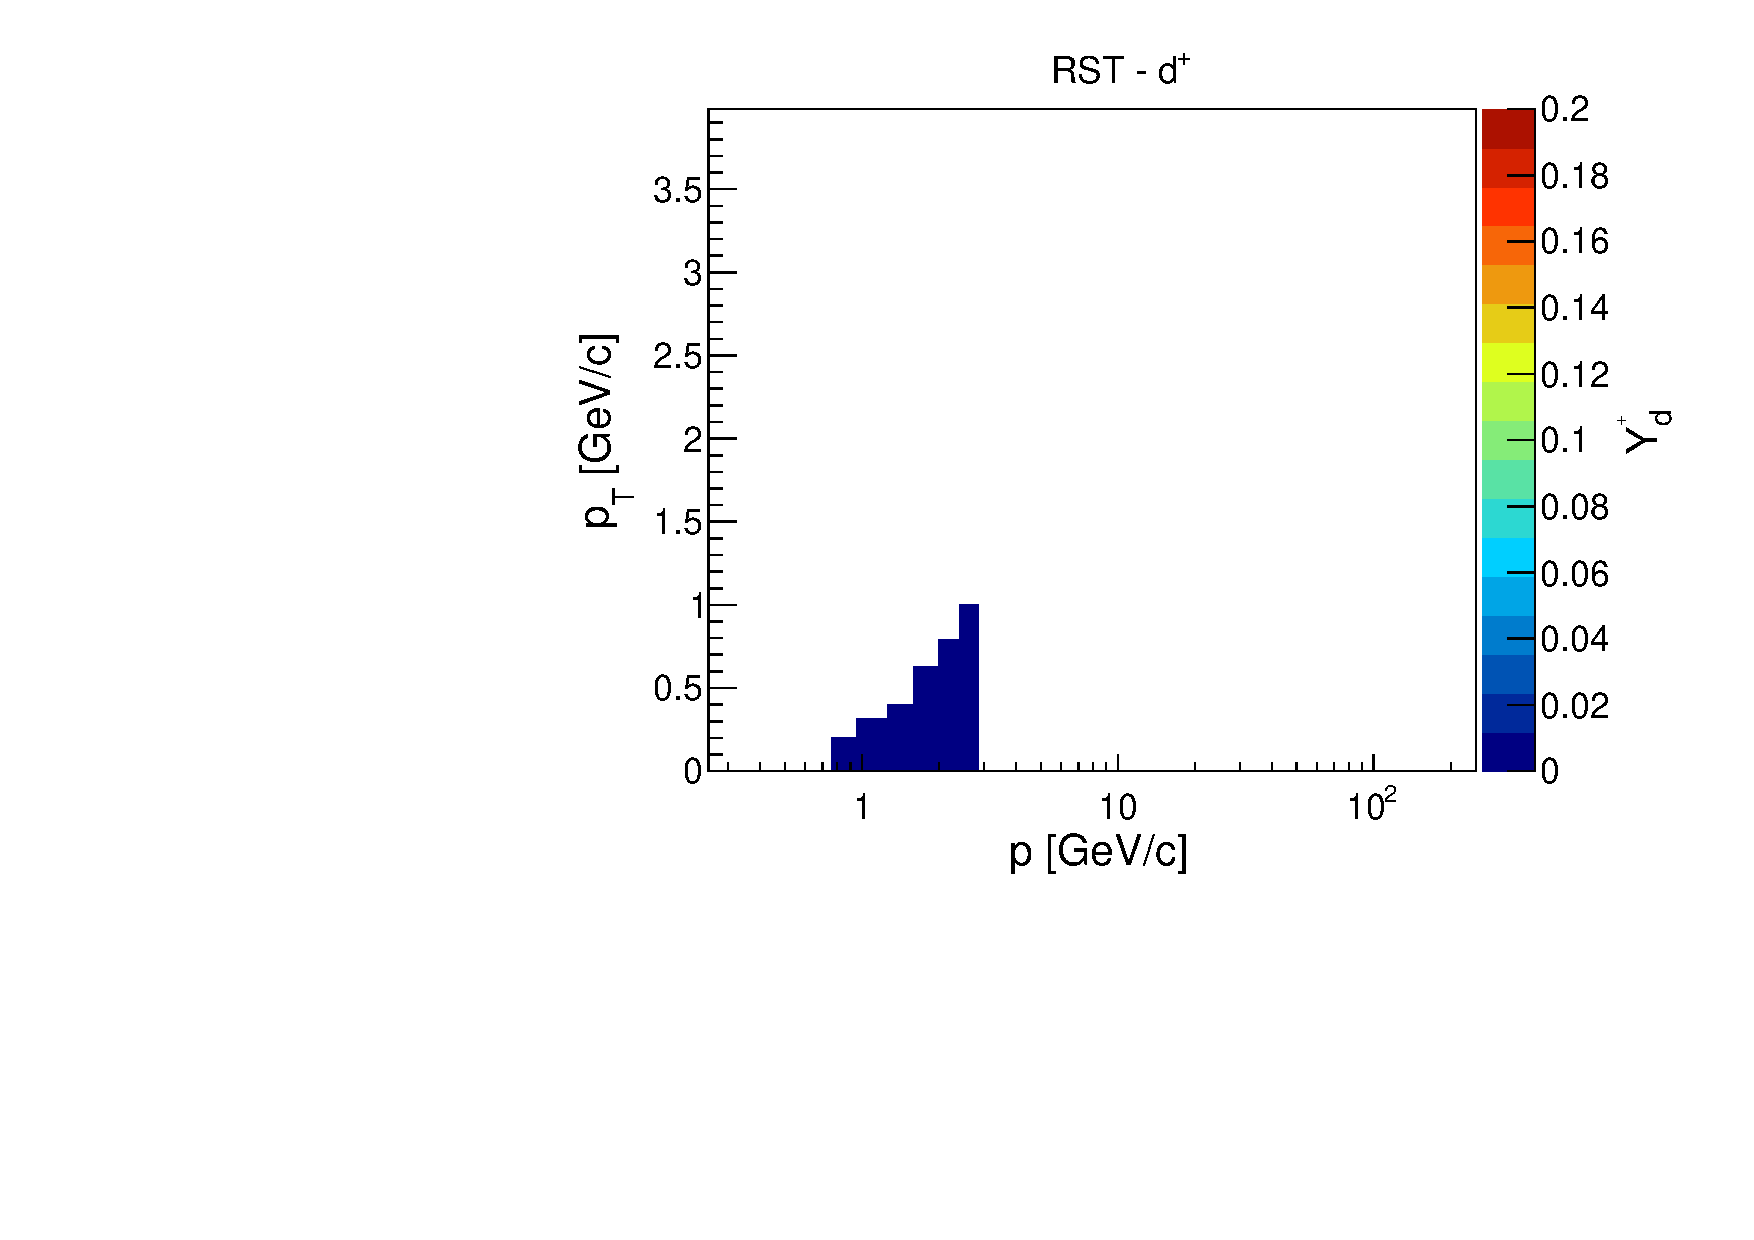
\includegraphics[clip, rviewport=0 0 1 0.94,width=0.4\textwidth]{dedx/fraction_158_fl0_v0_c1_p4}

  \caption{Particle fractions obtained from the fit of the RST dataset at 158 \GeVc.}
  \label{fig:hadron:dedx:fit:frac158r}
\end{figure}


%%%---------------------------------%%%%
\subsection{Simulated data ensembles, cuts and corrections}
\label{sec:hadron:dedx:sde}



The Simulated Data Ensembles (SDEs) are large sets of
simulations that reproduce the most relevant
features of the data and are fitted by following
exactly the same fit strategy described in~\cref{sec:hadron:dedx:fit}.
By analysing the fit results of the SDEs, we can evaluate the fit
performance in a statistical basis and then estimate the biases
and statistical uncertainties on the particle fractions. 

The construction of one individual simulation set of a SDE starts
by creating a new simulated tracks that reproduce the
properties of the data tracks. This means that the number of
tracks contained in a phase space bin, as well as its \pp, \pT and
\ncl distributions, is identical in the simulation and in the data.
The second step is to associate a particle type to each simulated track.
To do that we sample randomly one of the five possible types
by assigning them weights that are derived from the particle fractions
obtained from the \dedx fit of the data.
To avoid the statistical fluctuations on the fitted fractions,
a smoothing process was performed in which a 2-dimensional
forth-degree polynomial function was fitted to the fractions.
The fitted function is given by
\begin{equation}
  f(\pp,\pT) = \sum_{n=0}^{n<4} \sum_{m=0}^{m<4} a_{nm} (\log\pp)^n \pT^m,
  \label{eq:hadron:dedx:pol}
\end{equation}
where $a_{nm}$ are free parameters to be fitted.
The fit was performed by using a traditional $\chi^2$ method.
In~\cref{fig:hadron:dedx:fit:fakeyield} we show few examples
of the \pT projection of the fractions and the fitted
polynomial function. 


%%%%%%%%%% FAKE YIELD %%%%%%%%%%%%%%
\begin{figure}[!ht]
  \centering
  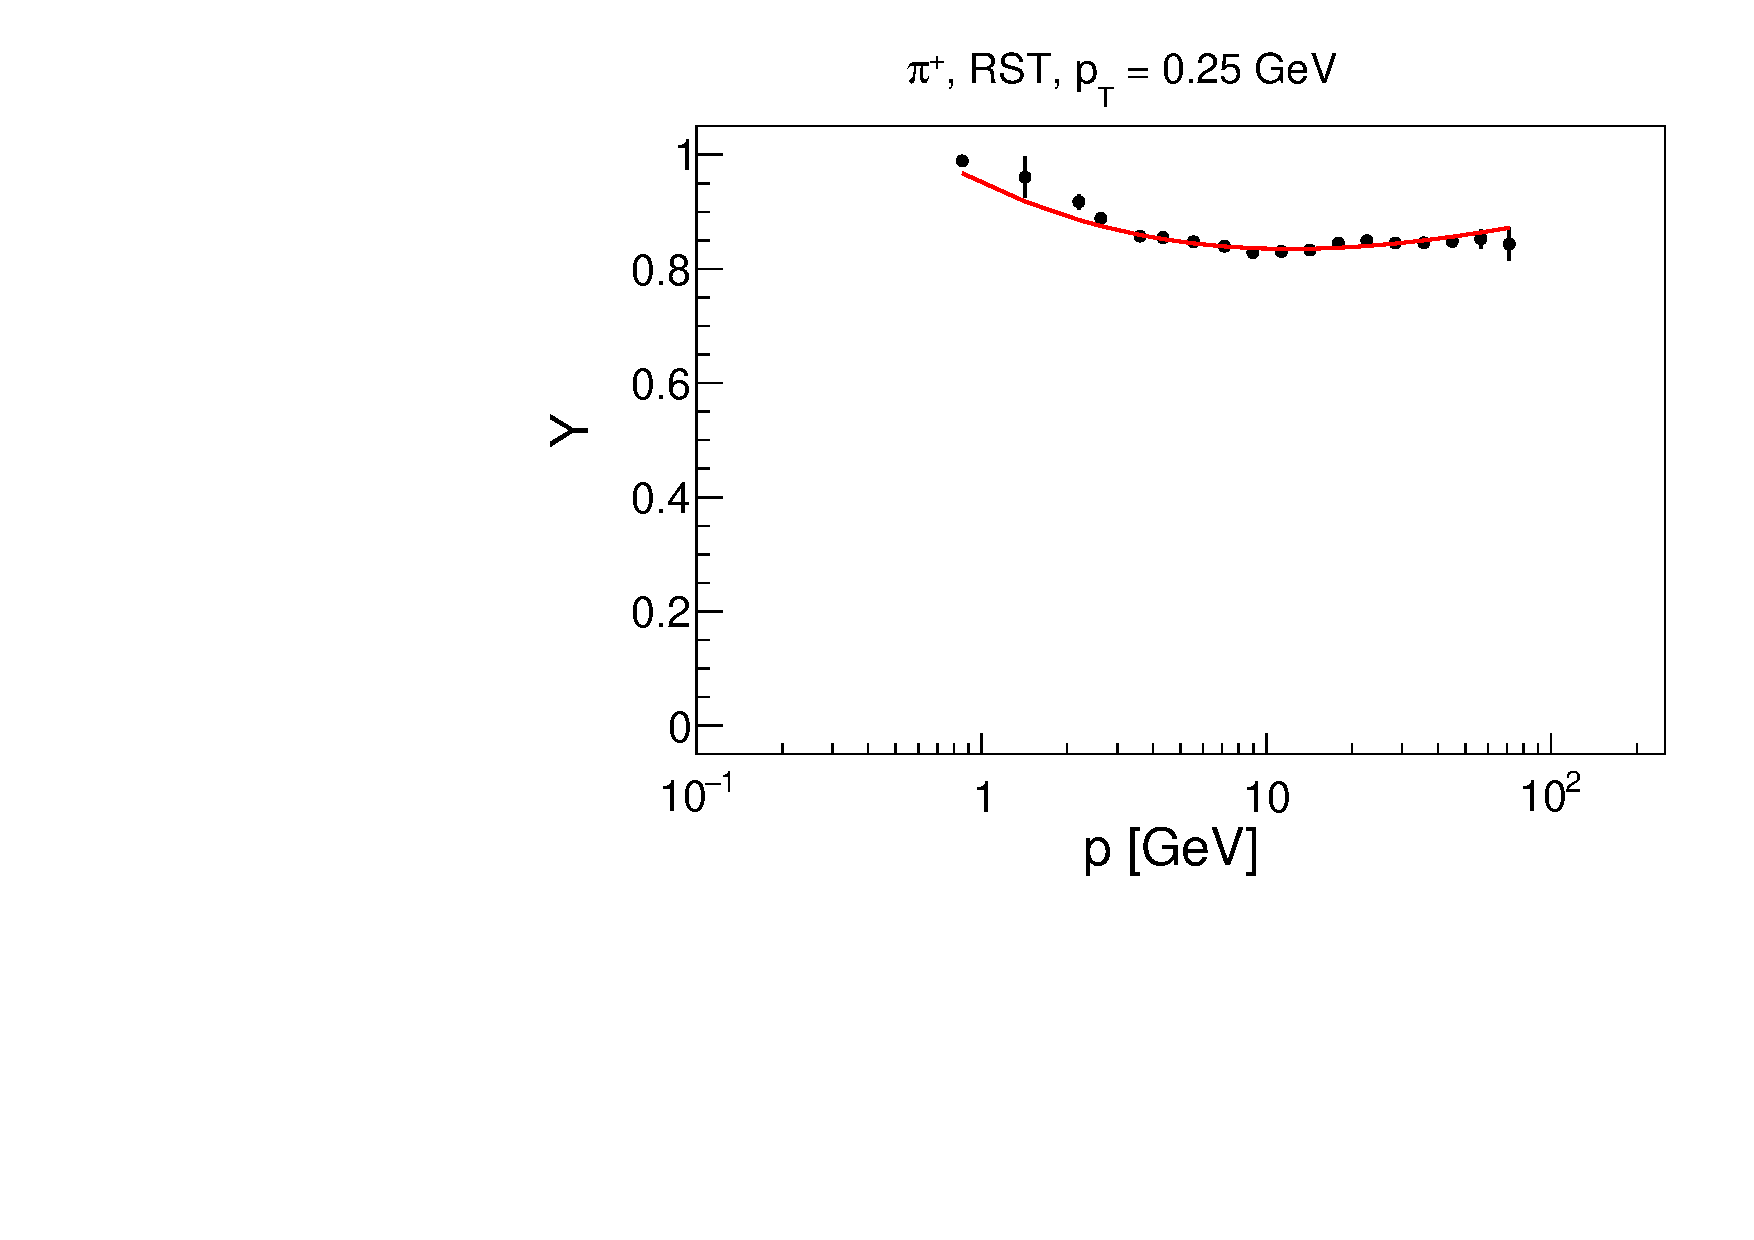
\includegraphics[clip, rviewport=0 0 1 1,width=0.4\textwidth]{dedx/fake_yield_example_158}
  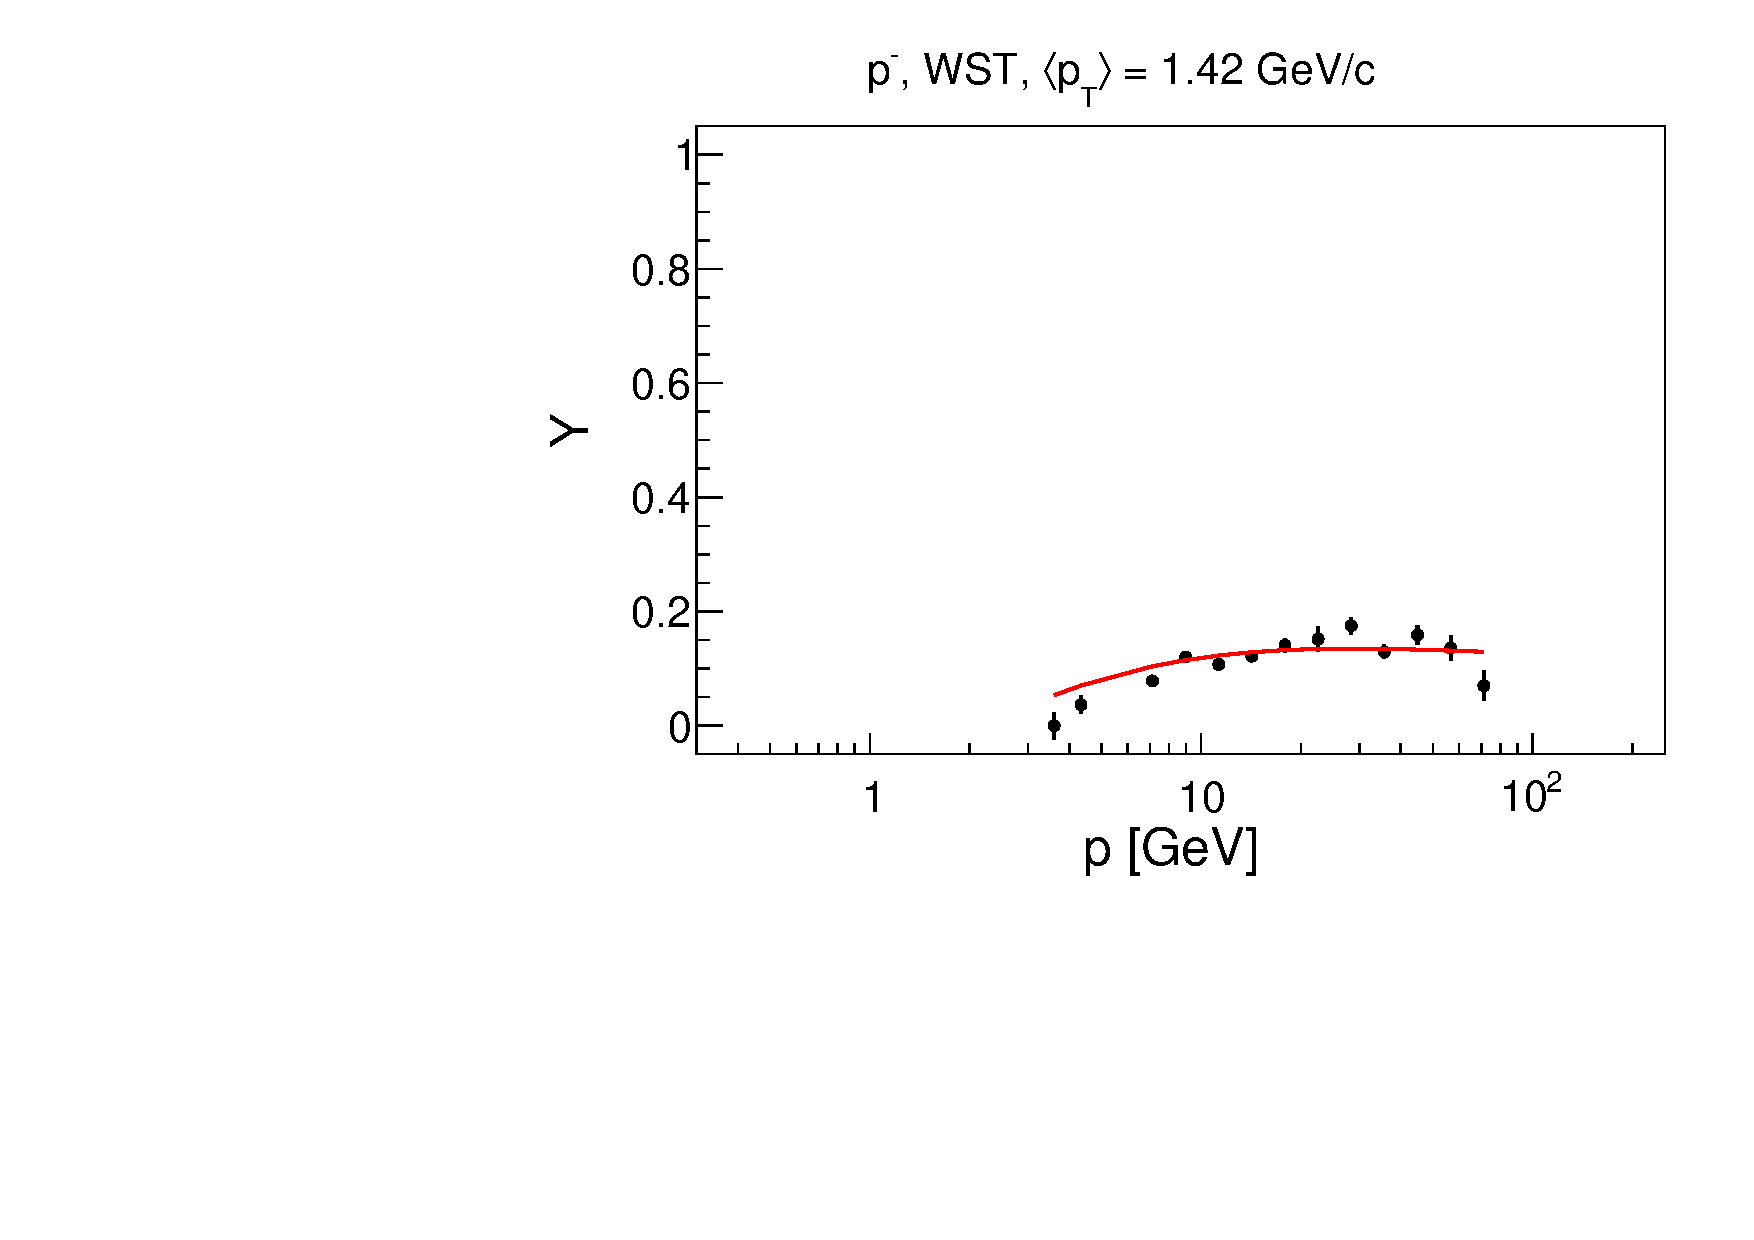
\includegraphics[clip, rviewport=0 0 1 1,width=0.4\textwidth]{dedx/fake_yield_example_two_158}

  \vspace{0.5cm}
  
  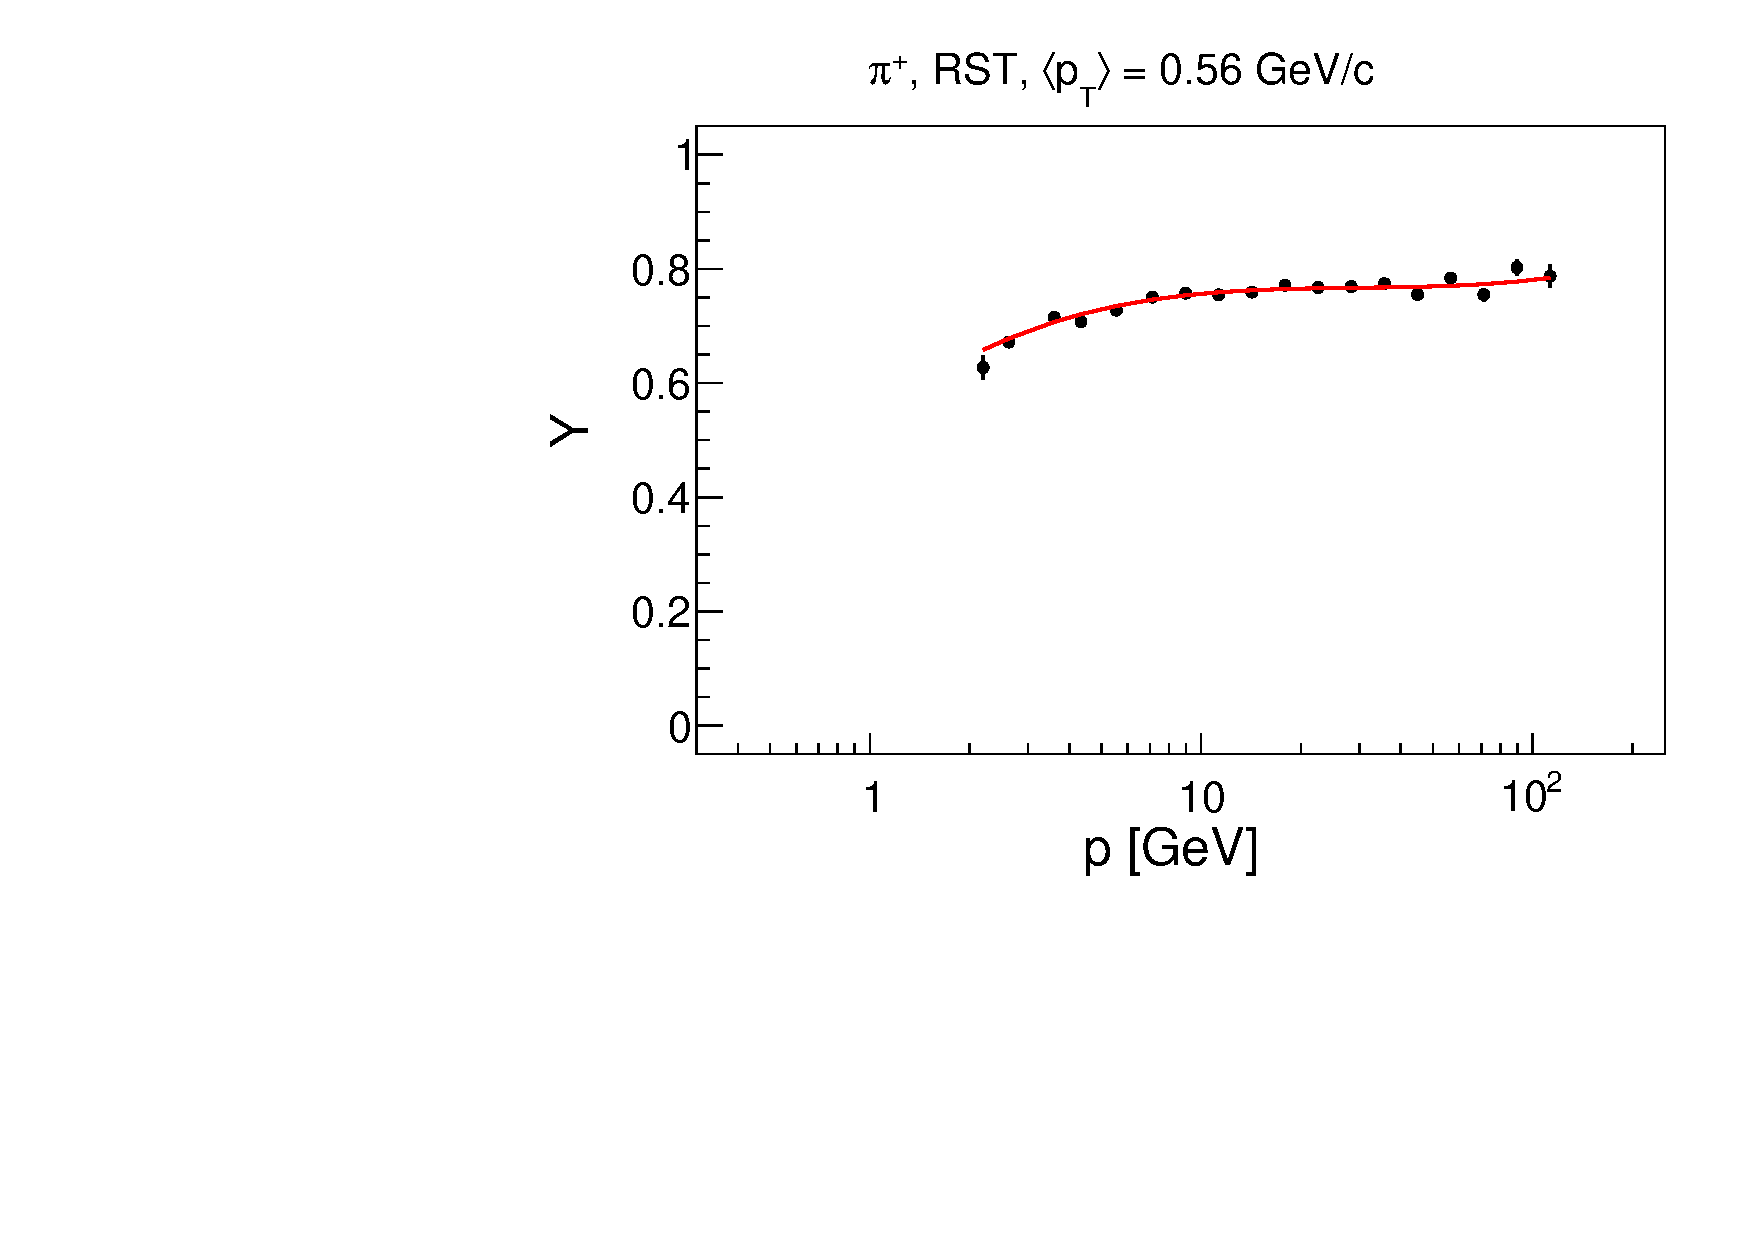
\includegraphics[clip, rviewport=0 0 1 1,width=0.4\textwidth]{dedx/fake_yield_example_350}
  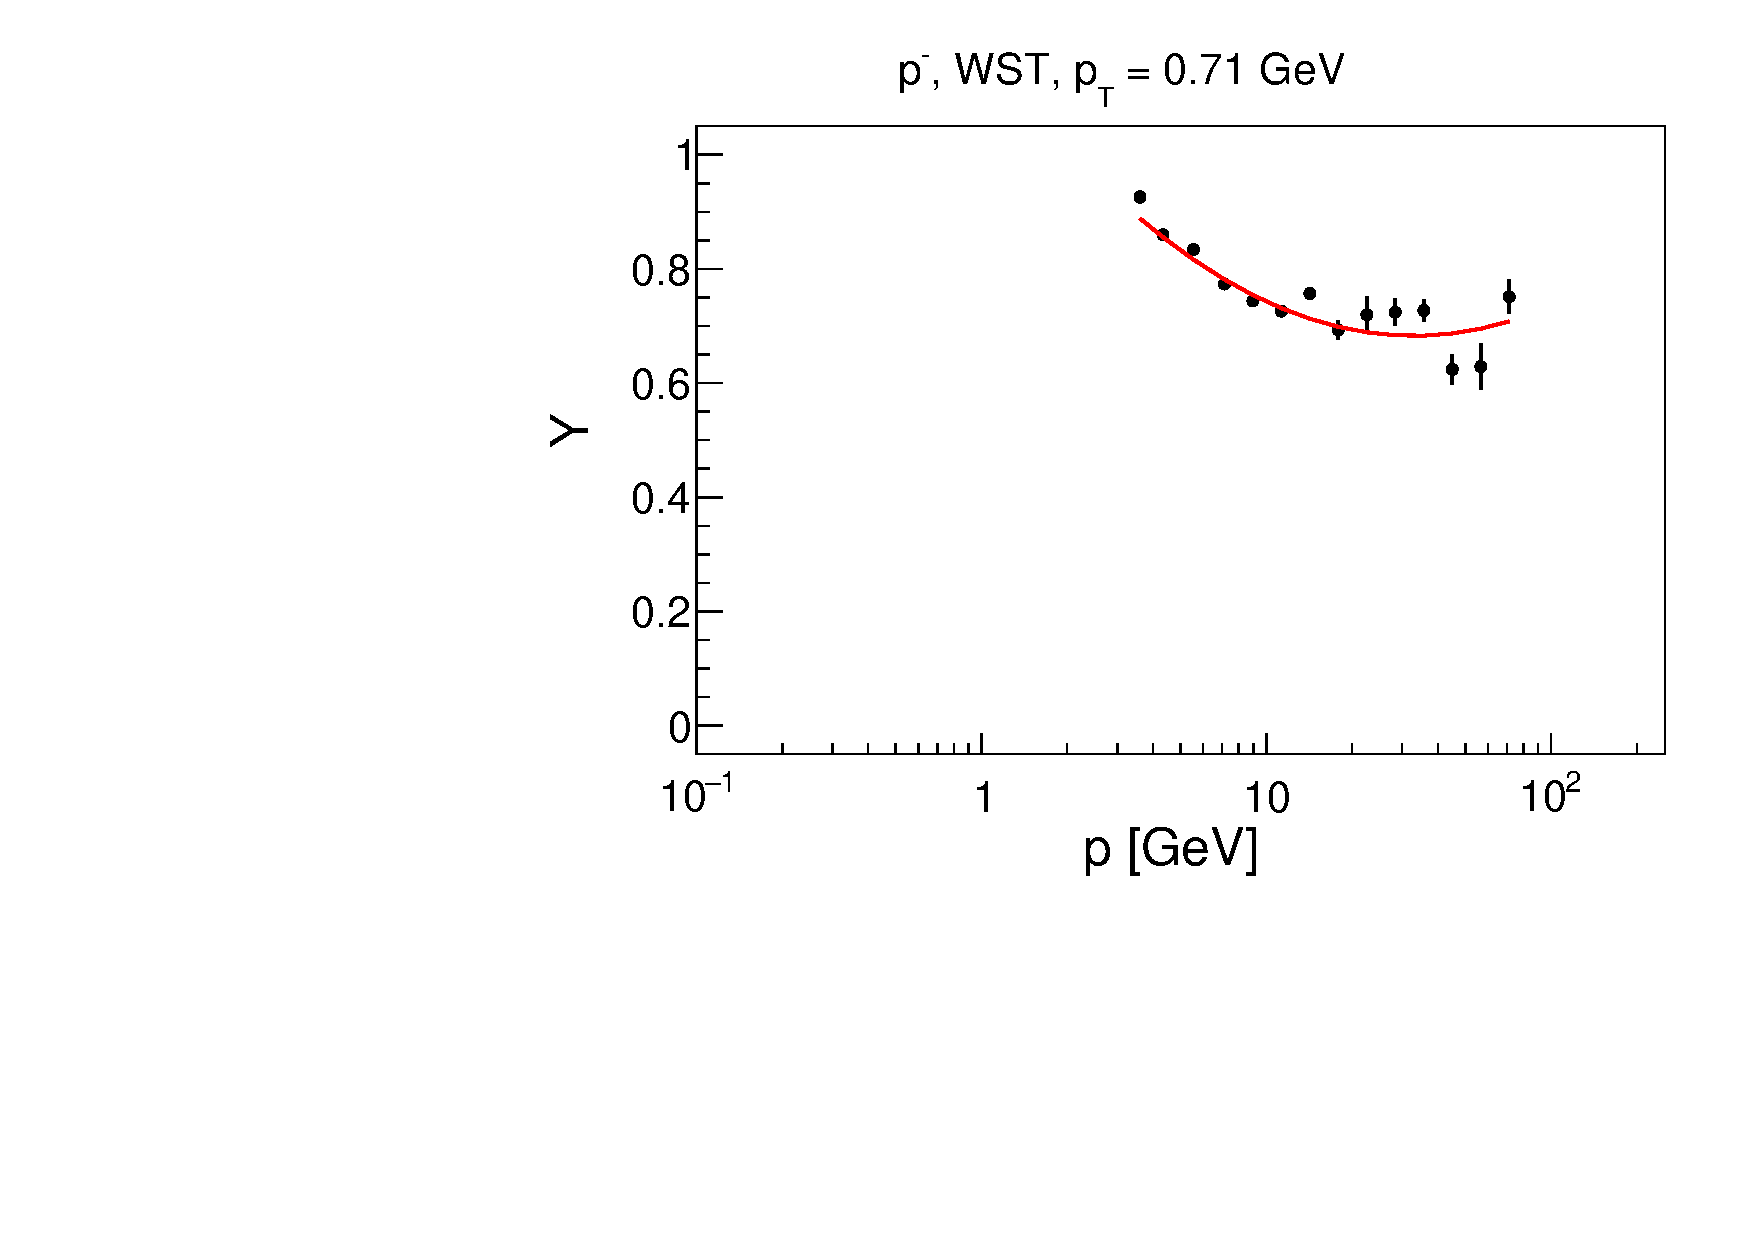
\includegraphics[clip, rviewport=0 0 1 1,width=0.4\textwidth]{dedx/fake_yield_example_two_350}

  \caption{Examples of the parametrization of the particle fractions to be used to create the Simulated Data Ensembles. The plots on the top and on the bottom are for the 158 and 350 \GeVc dataset, respectively.}
  \label{fig:hadron:dedx:fit:fakeyield}
\end{figure}


After sampling a particle type, the \dedx associated to each
track is sampled by following the \dedx model.
The model parameters are set as the ones obtained by the \dedx fit
of the data that are shown in~\cref{sec:hadron:dedx:fitresults}.
A set of $\approx 1000$ simulated sets, for each beam energy,
were created by following the description above and
fitted afterwards. As the result, we obtain the distributions
of the fitted fractions for each particle and phase space bin.

First we can evaluate the relative standard deviation,
defined as $\sigma_r = \sigma_Y/\langle Y\rangle$, where
$\sigma_Y$ is the standard deviation of the fraction $Y$
and $\langle Y \rangle$ is its average value.
In~\cref{fig:hadron:dedx:fit:fake:relsig158r} we show
one example of $\sigma_r$ for the RST and 158 \GeVc case.
The remaining cases are shown
in~\cref{fig:hadron:dedx:fit:fake:relsig158w,fig:hadron:dedx:fit:fake:relsig350r,fig:hadron:dedx:fit:fake:relsig350w}. Only \pions, \kaons and \protons are shown
because these are the particles of interested of this analysis.
Second, we can evaluate the relative bias, defined as
$\delta_r = \langle \Delta Y/ Y \rangle$, where $\Delta Y$
is the difference between the fitted and the true fraction,
being the true fraction computed while the particle types
of each track are sampled.
In~\cref{fig:hadron:dedx:fit:fake:reldev158r} we show examples
of $\delta_r$ for RST and 158 \GeVc case, while the remaning
cases are shown
in~\cref{fig:hadron:dedx:fit:fake:reldev158w,fig:hadron:dedx:fit:fake:reldev350r,fig:hadron:dedx:fit:fake:reldev350w}.

%%%%%%%%%% FAKE REL SIG %%%%%%%%%%%%%%
\begin{figure}[!ht]
  \centering
  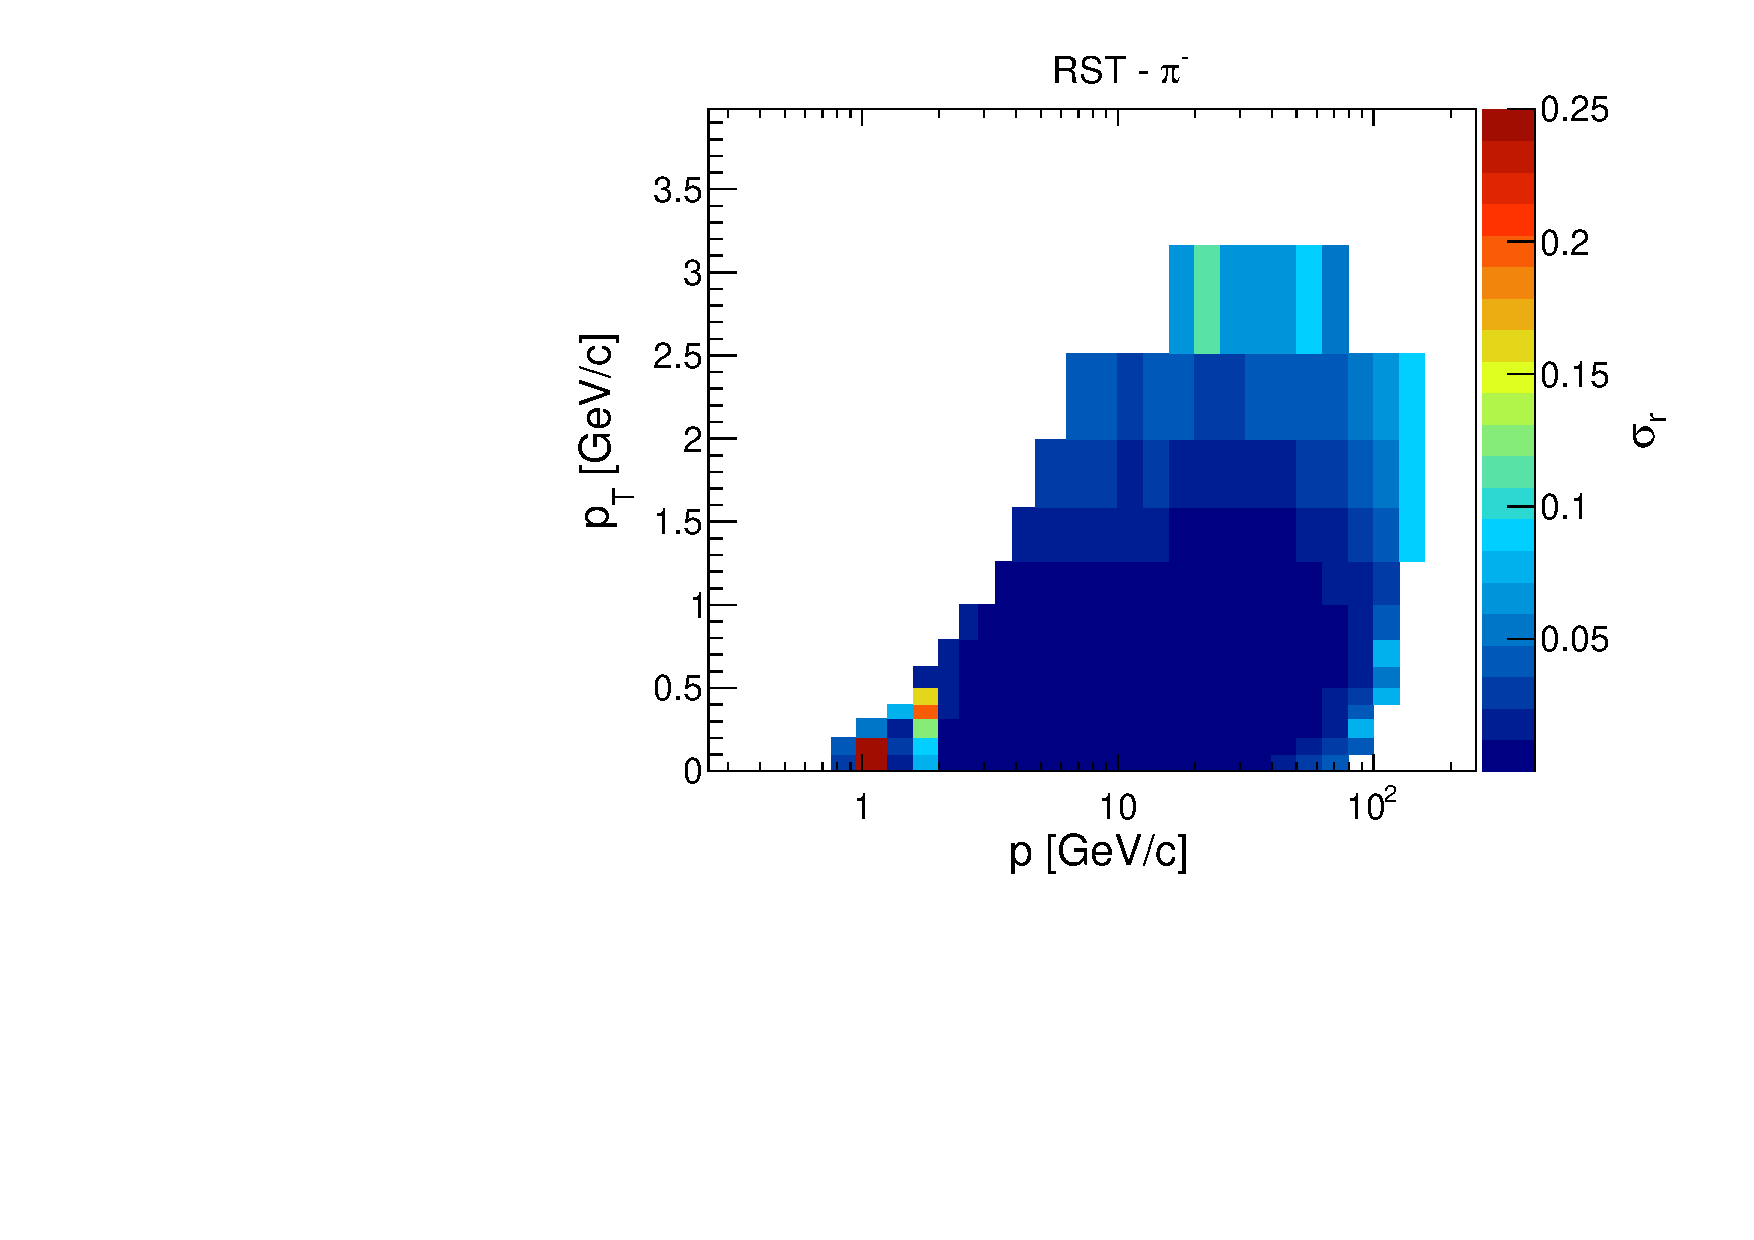
\includegraphics[clip, rviewport=0 0.13 1 0.94,width=0.4\textwidth]{dedx/fake_rel_sig_158_fl0_v0_c0_p1}
  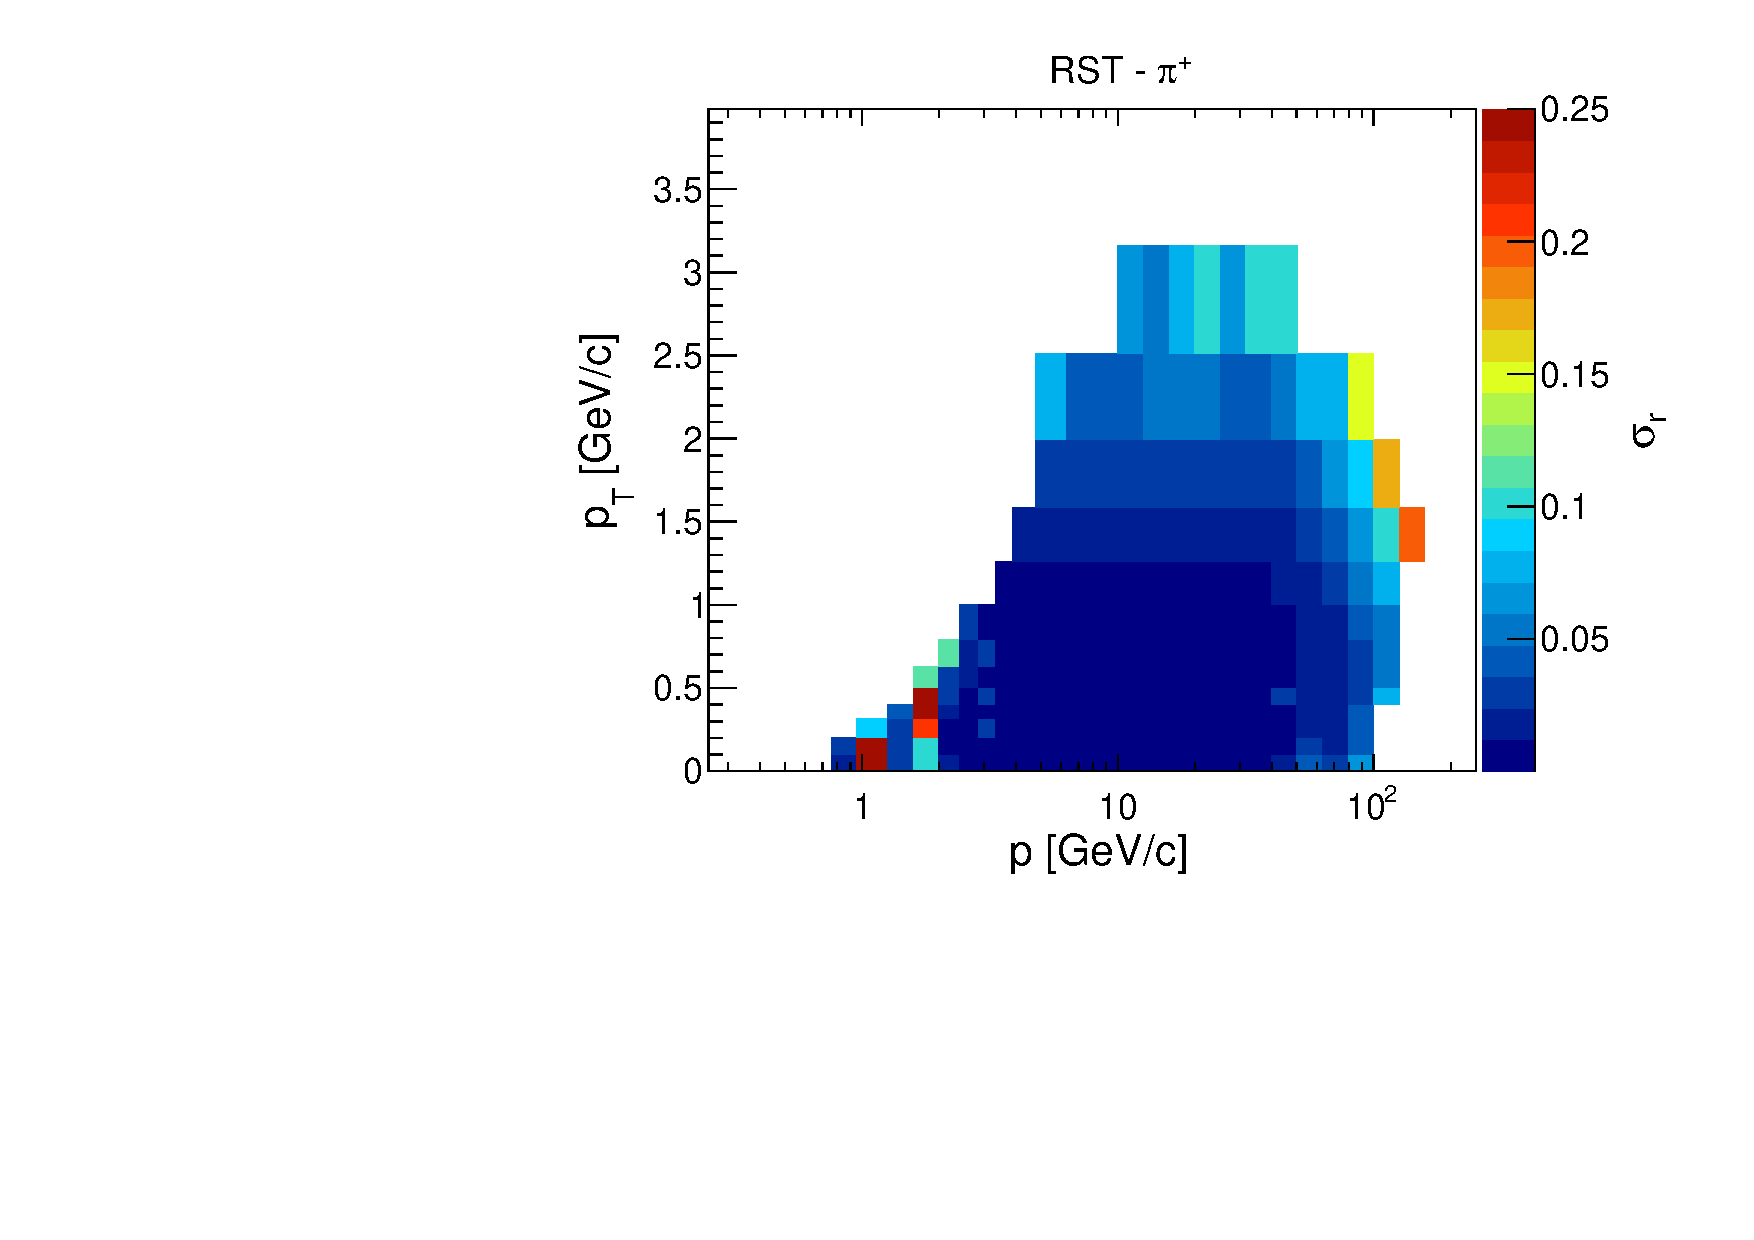
\includegraphics[clip, rviewport=0 0.13 1 0.94,width=0.4\textwidth]{dedx/fake_rel_sig_158_fl0_v0_c1_p1}

  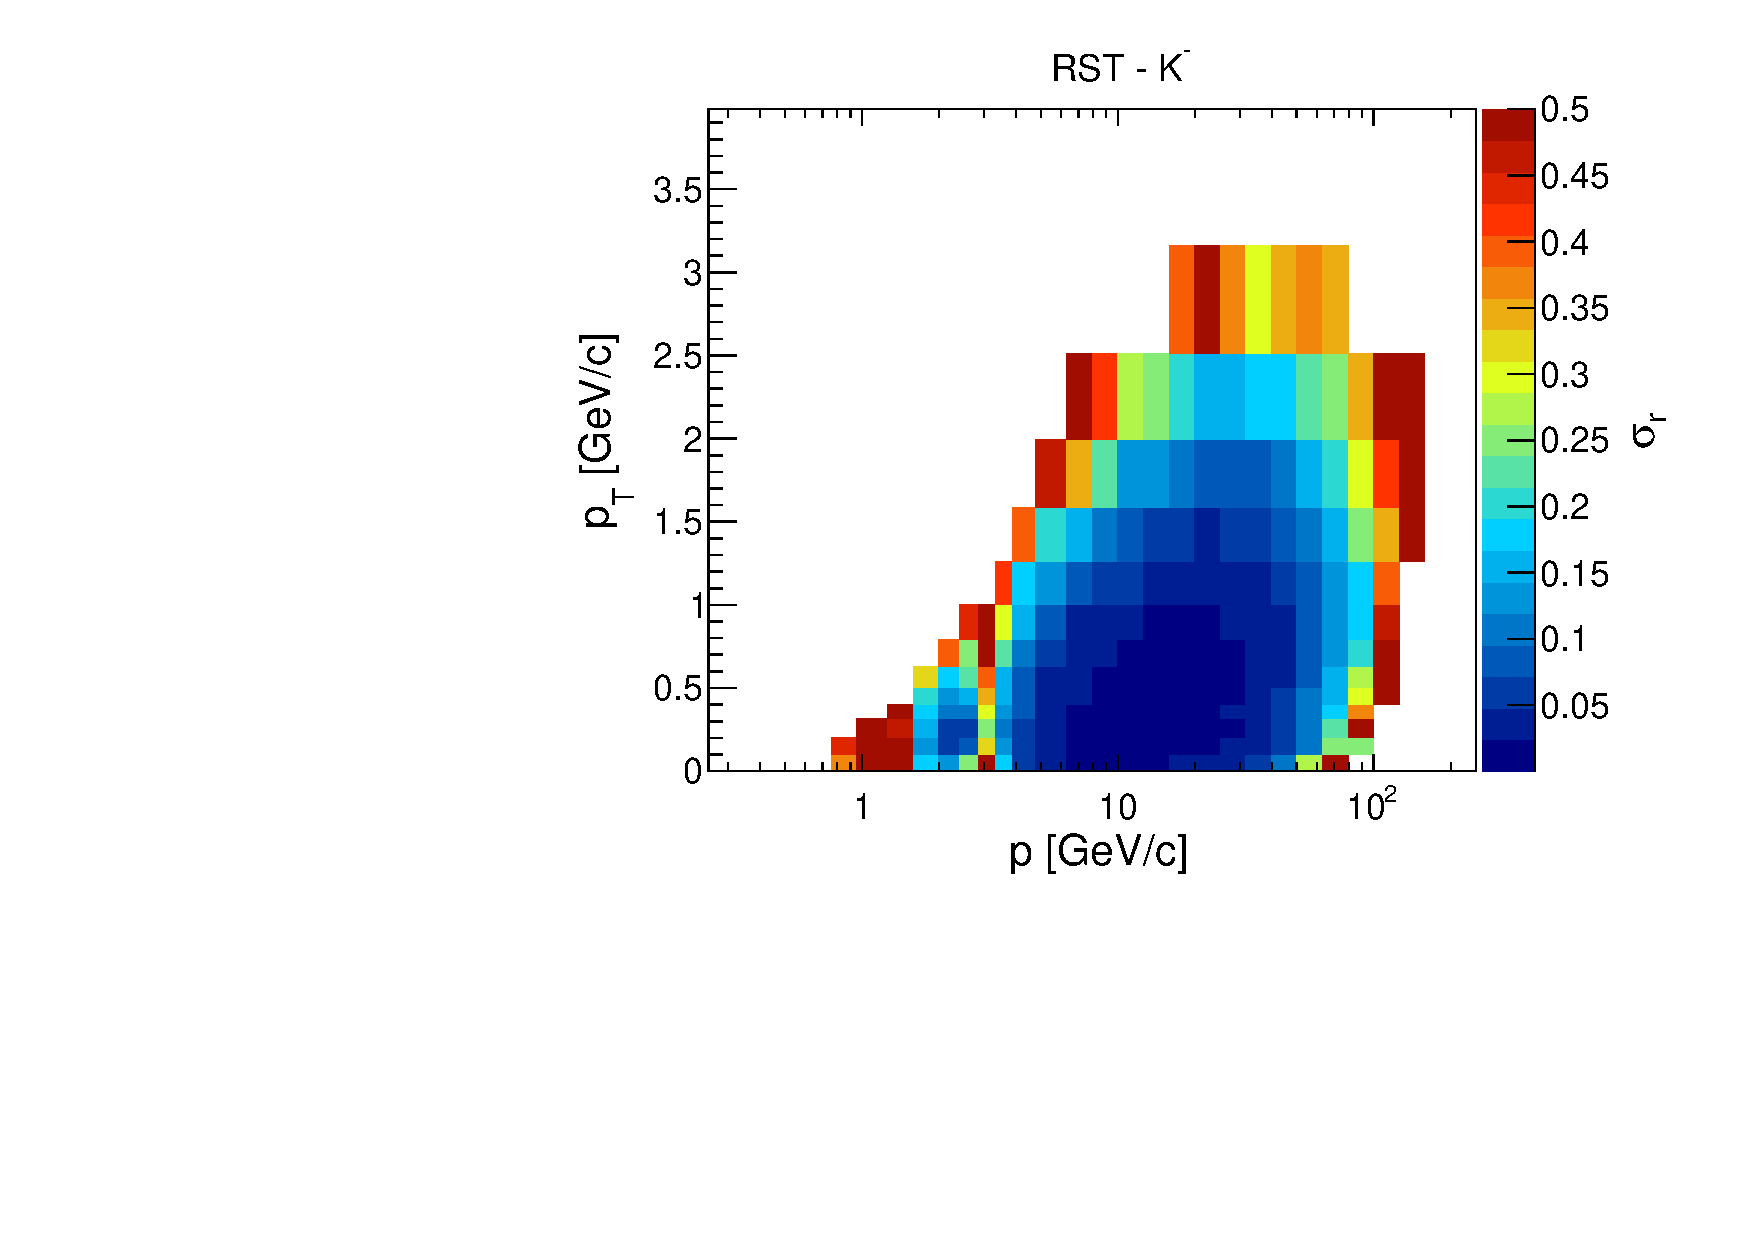
\includegraphics[clip, rviewport=0 0.13 1 0.94,width=0.4\textwidth]{dedx/fake_rel_sig_158_fl0_v0_c0_p2}
  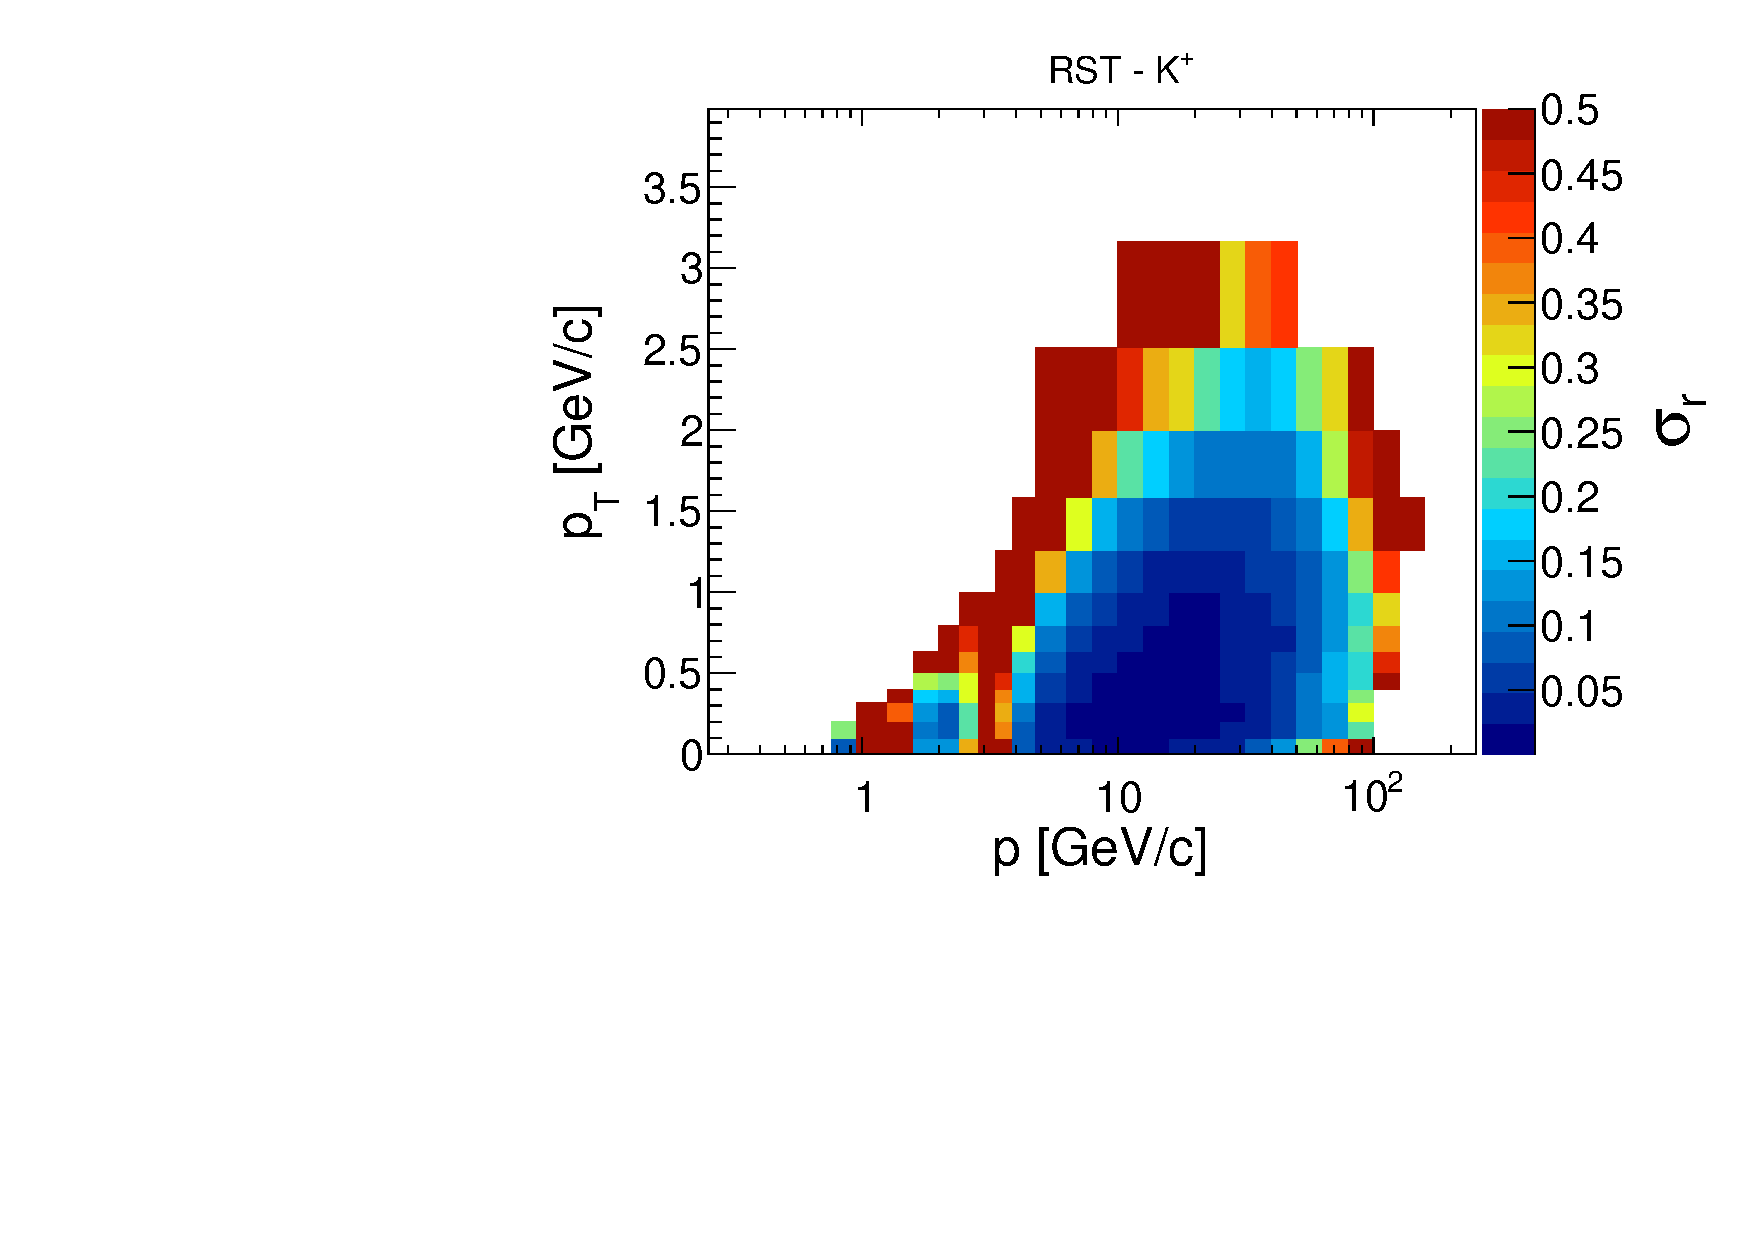
\includegraphics[clip, rviewport=0 0.13 1 0.94,width=0.4\textwidth]{dedx/fake_rel_sig_158_fl0_v0_c1_p2}

  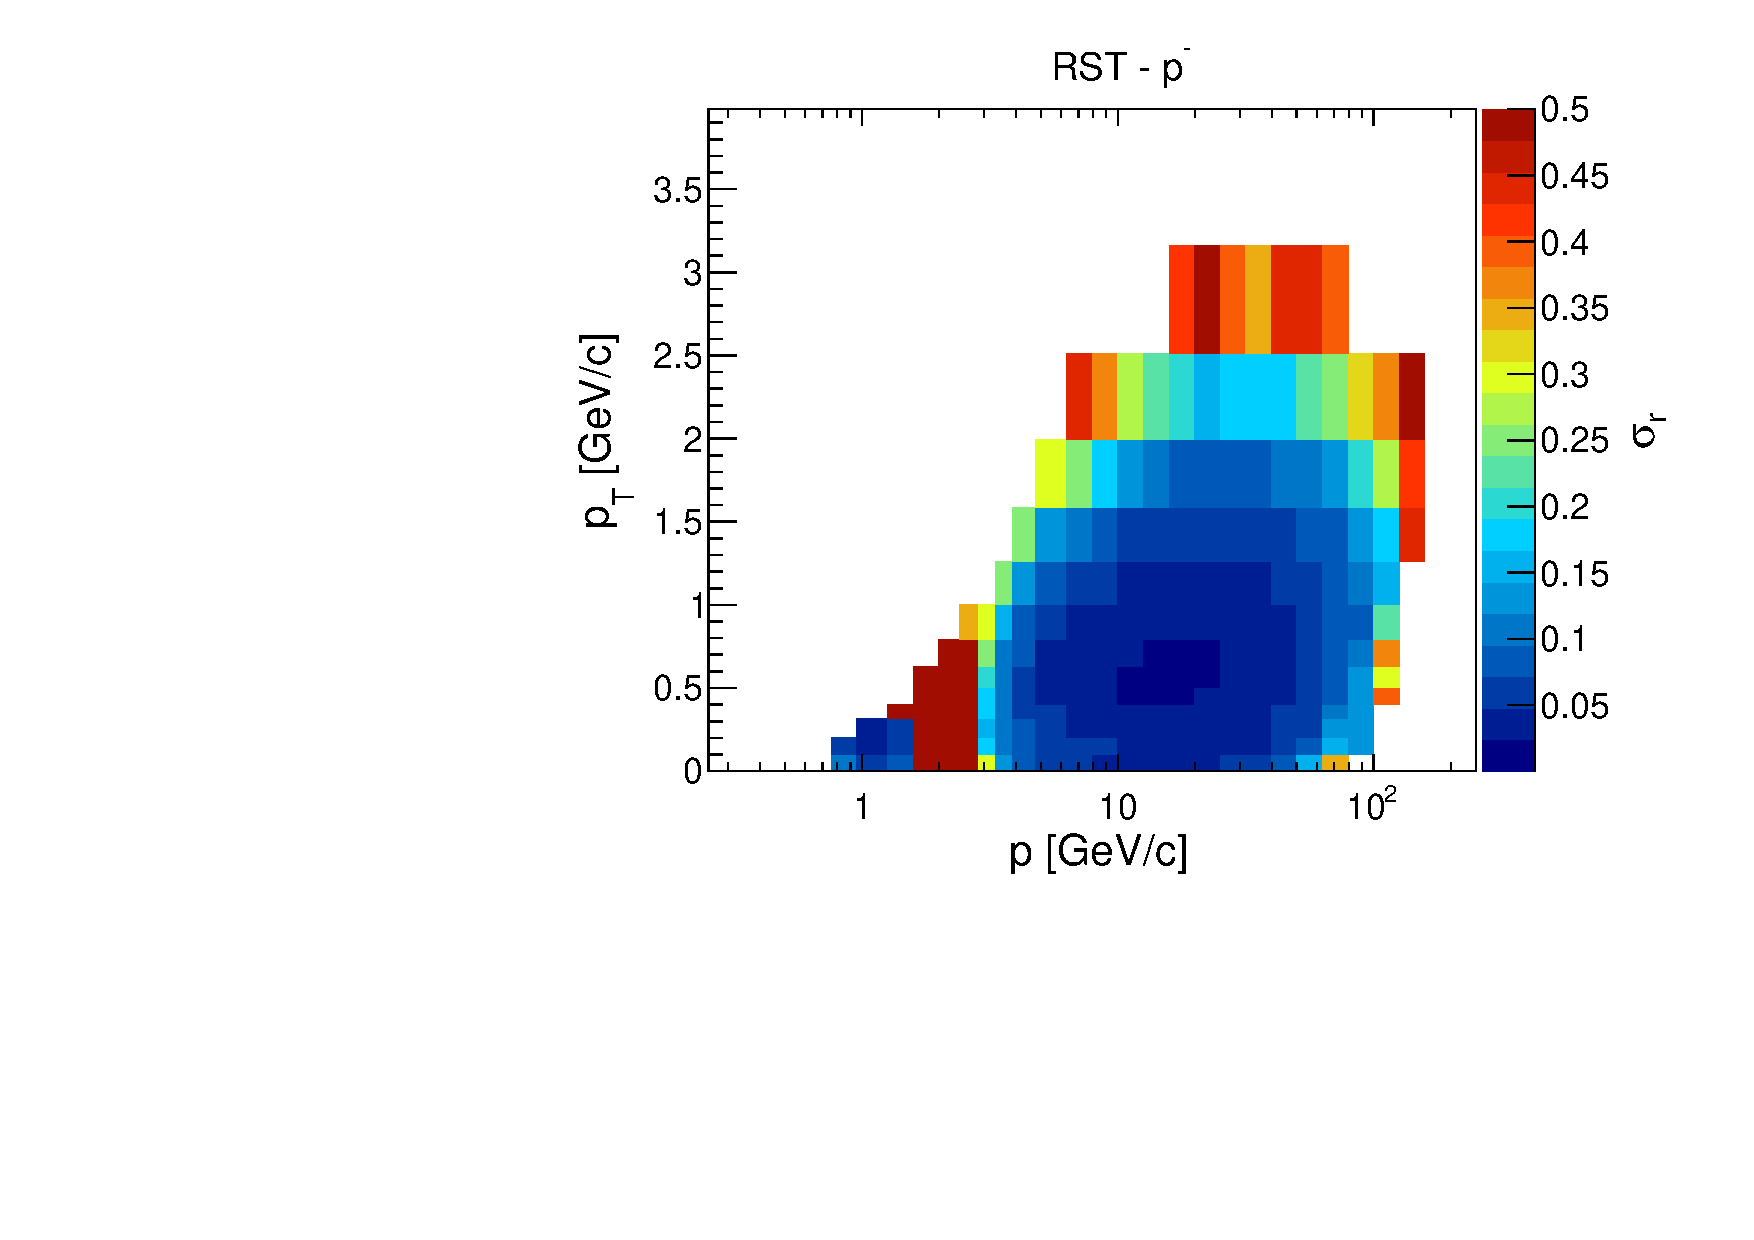
\includegraphics[clip, rviewport=0 0 1 0.94,width=0.4\textwidth]{dedx/fake_rel_sig_158_fl0_v0_c0_p3}
  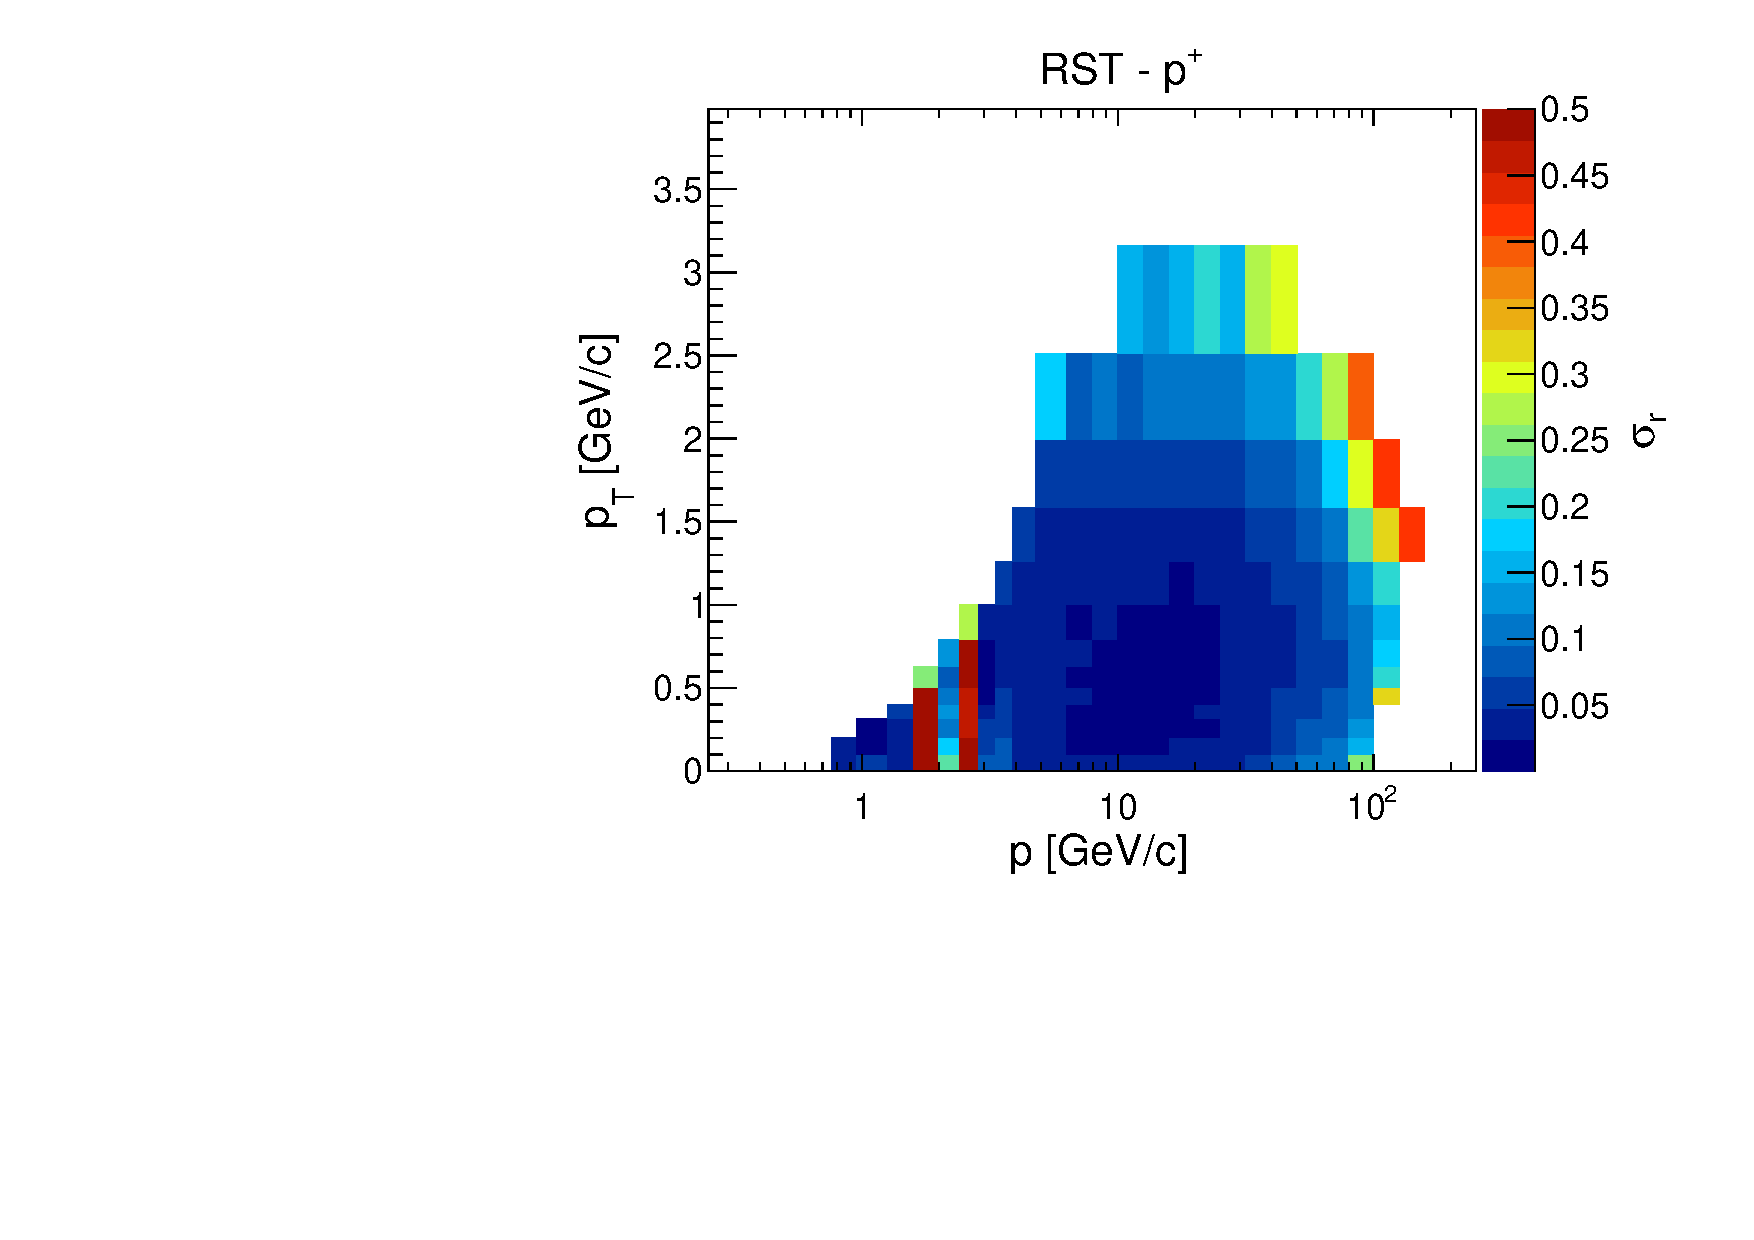
\includegraphics[clip, rviewport=0 0 1 0.94,width=0.4\textwidth]{dedx/fake_rel_sig_158_fl0_v0_c1_p3}


  \caption{Relative standard deviation of the particle fractions obtained with SDEs for RST and 158 \GeVc dataset.}
  \label{fig:hadron:dedx:fit:fake:relsig158r}
\end{figure}


%%%%%%%%%% FAKE REL DEV %%%%%%%%%%%%%%
\begin{figure}[!ht]
  \centering
  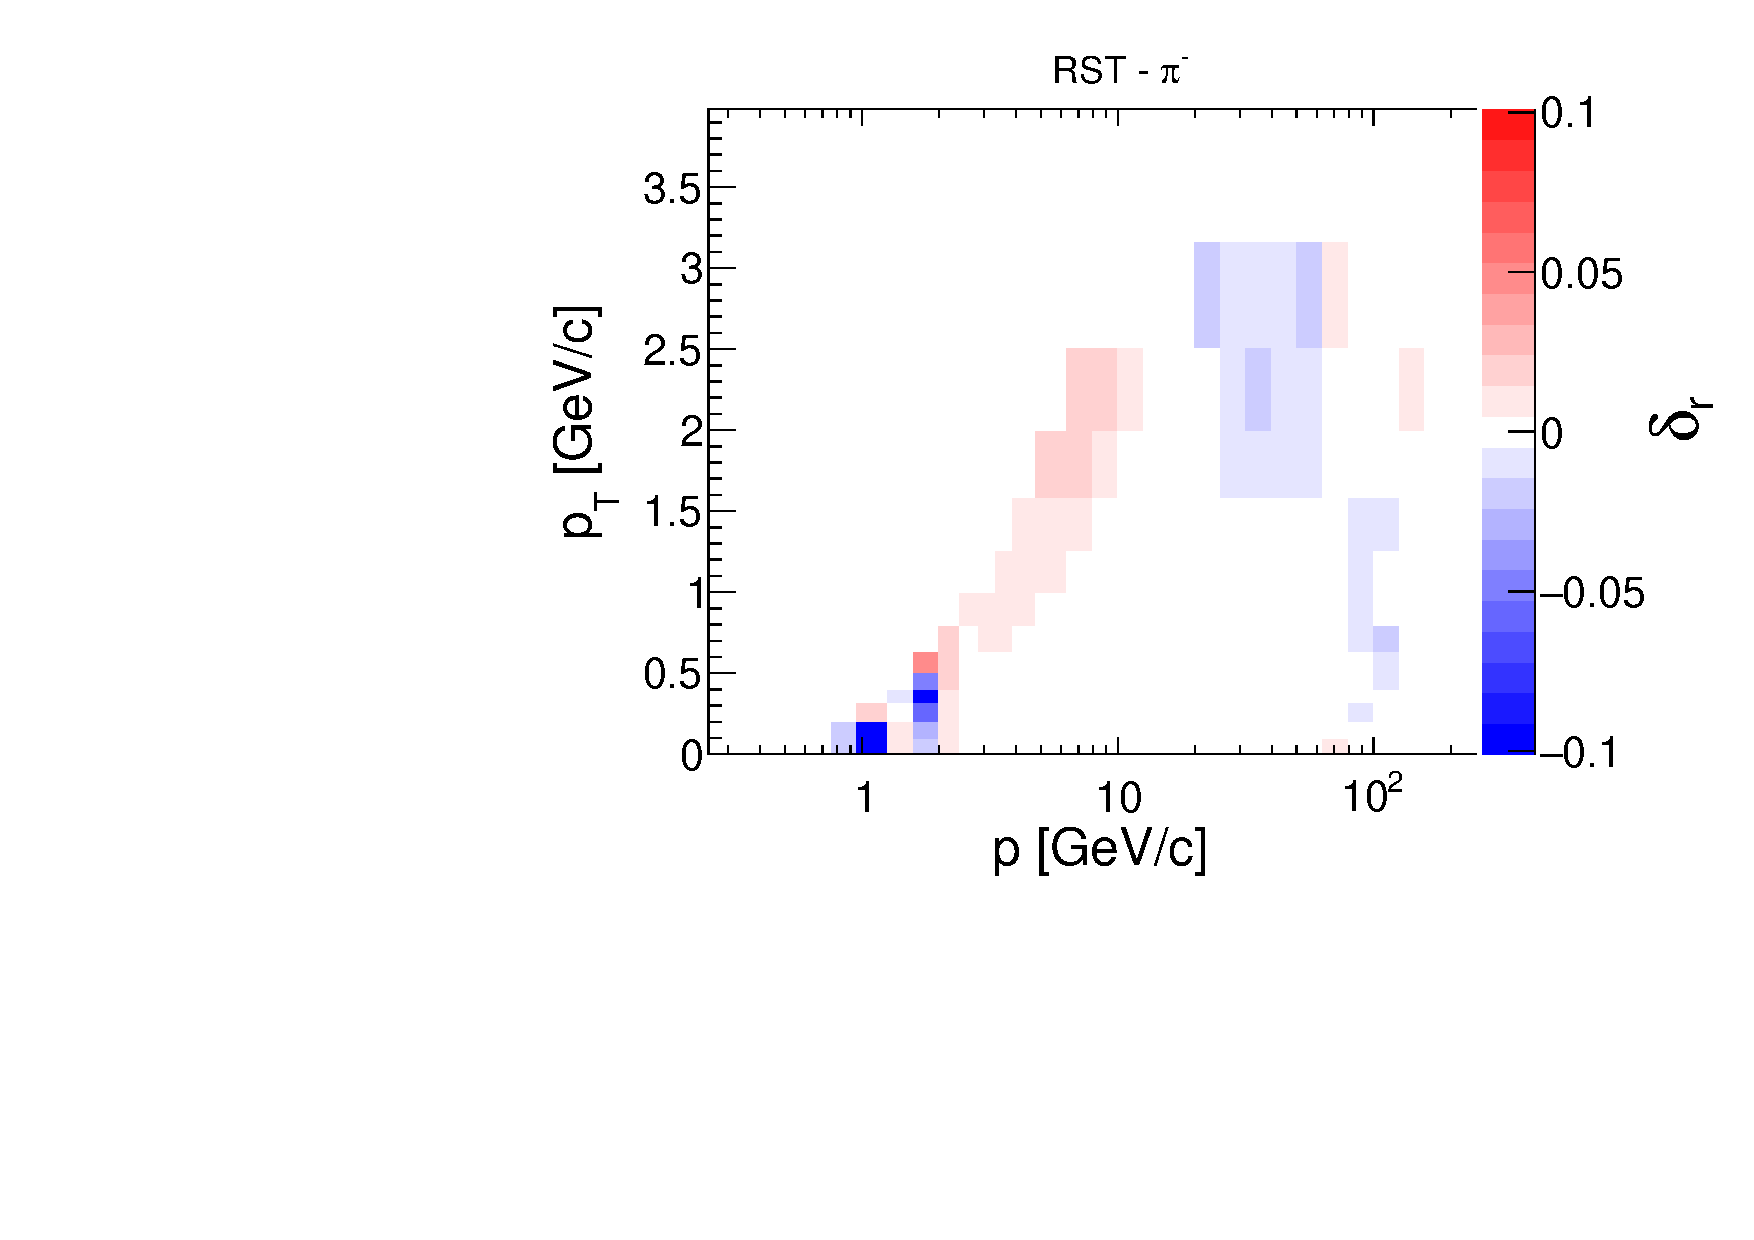
\includegraphics[clip, rviewport=0 0.13 1 0.94,width=0.4\textwidth]{dedx/fake_rel_dev_158_fl0_v0_c0_p1}
  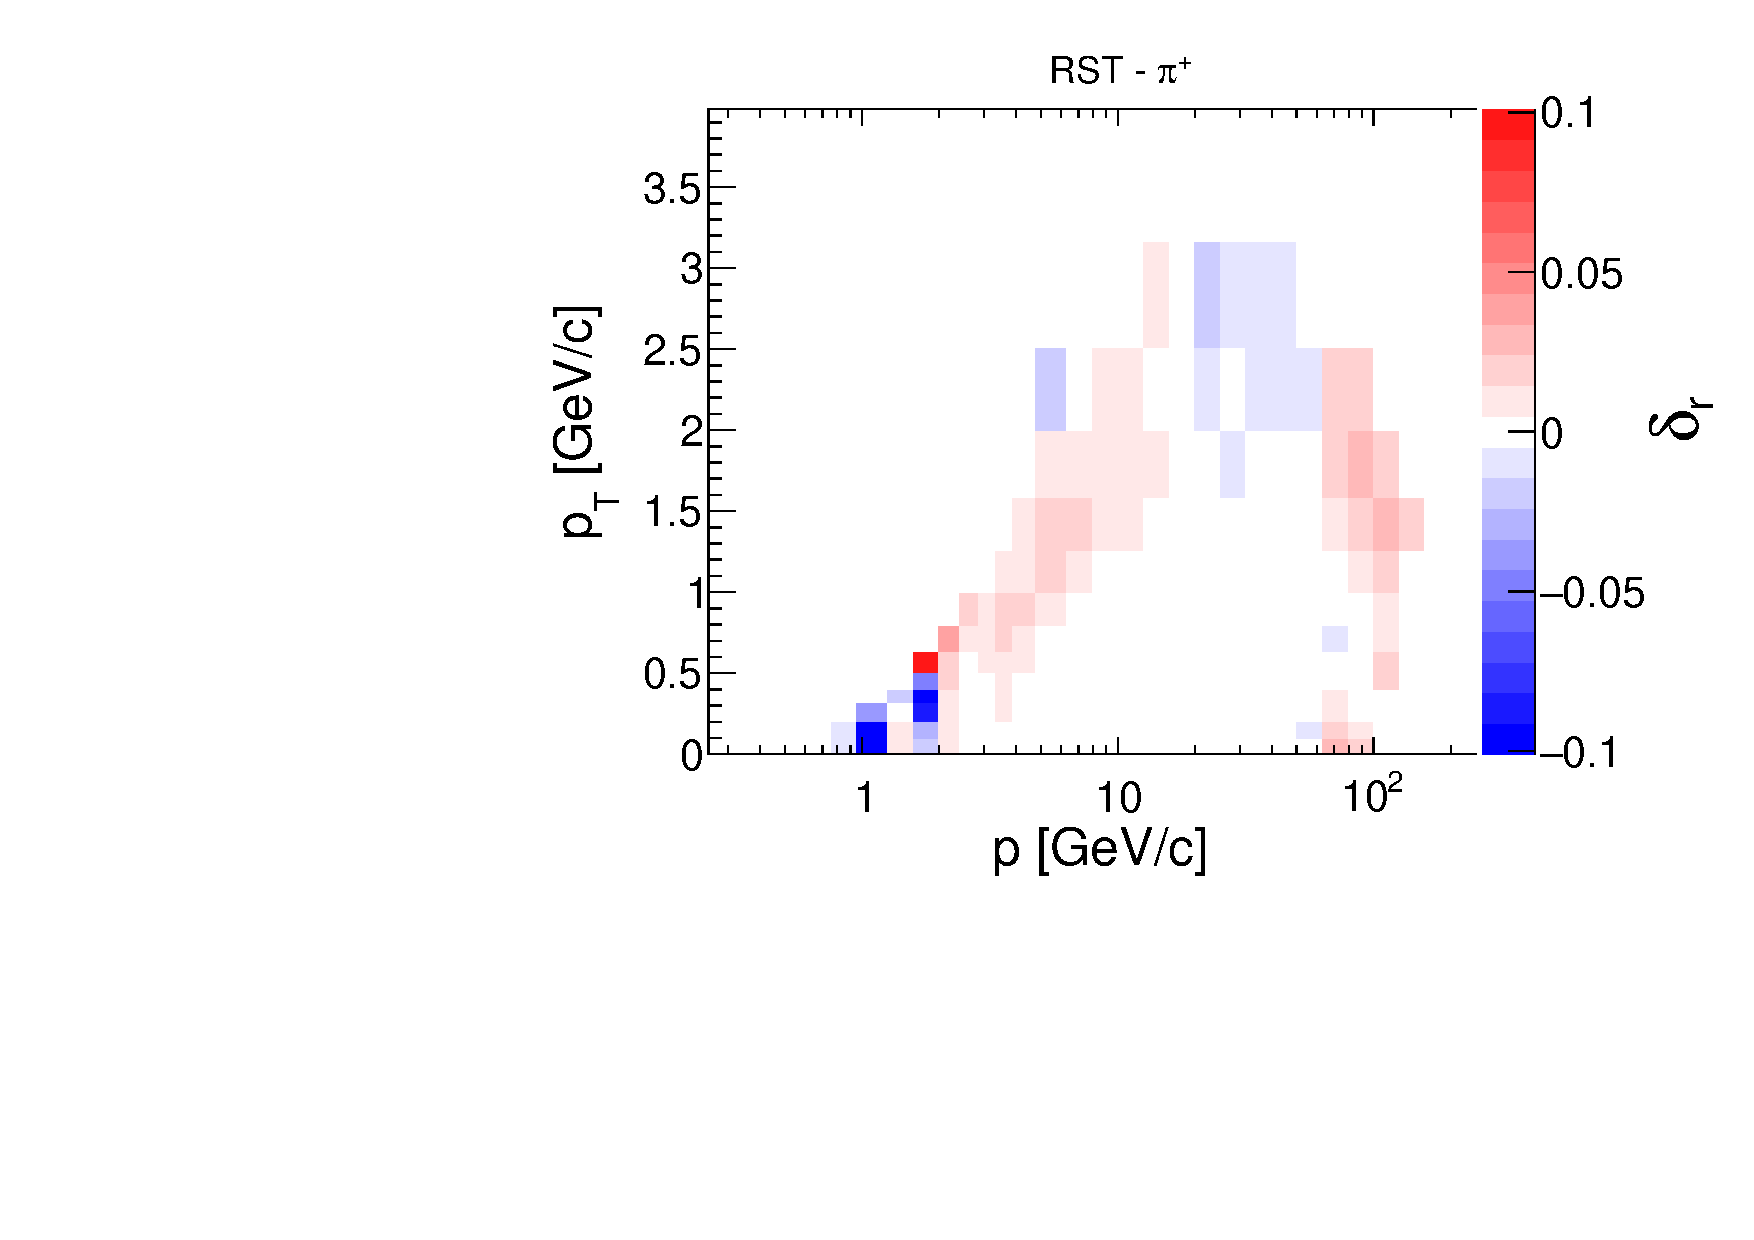
\includegraphics[clip, rviewport=0 0.13 1 0.94,width=0.4\textwidth]{dedx/fake_rel_dev_158_fl0_v0_c1_p1}

  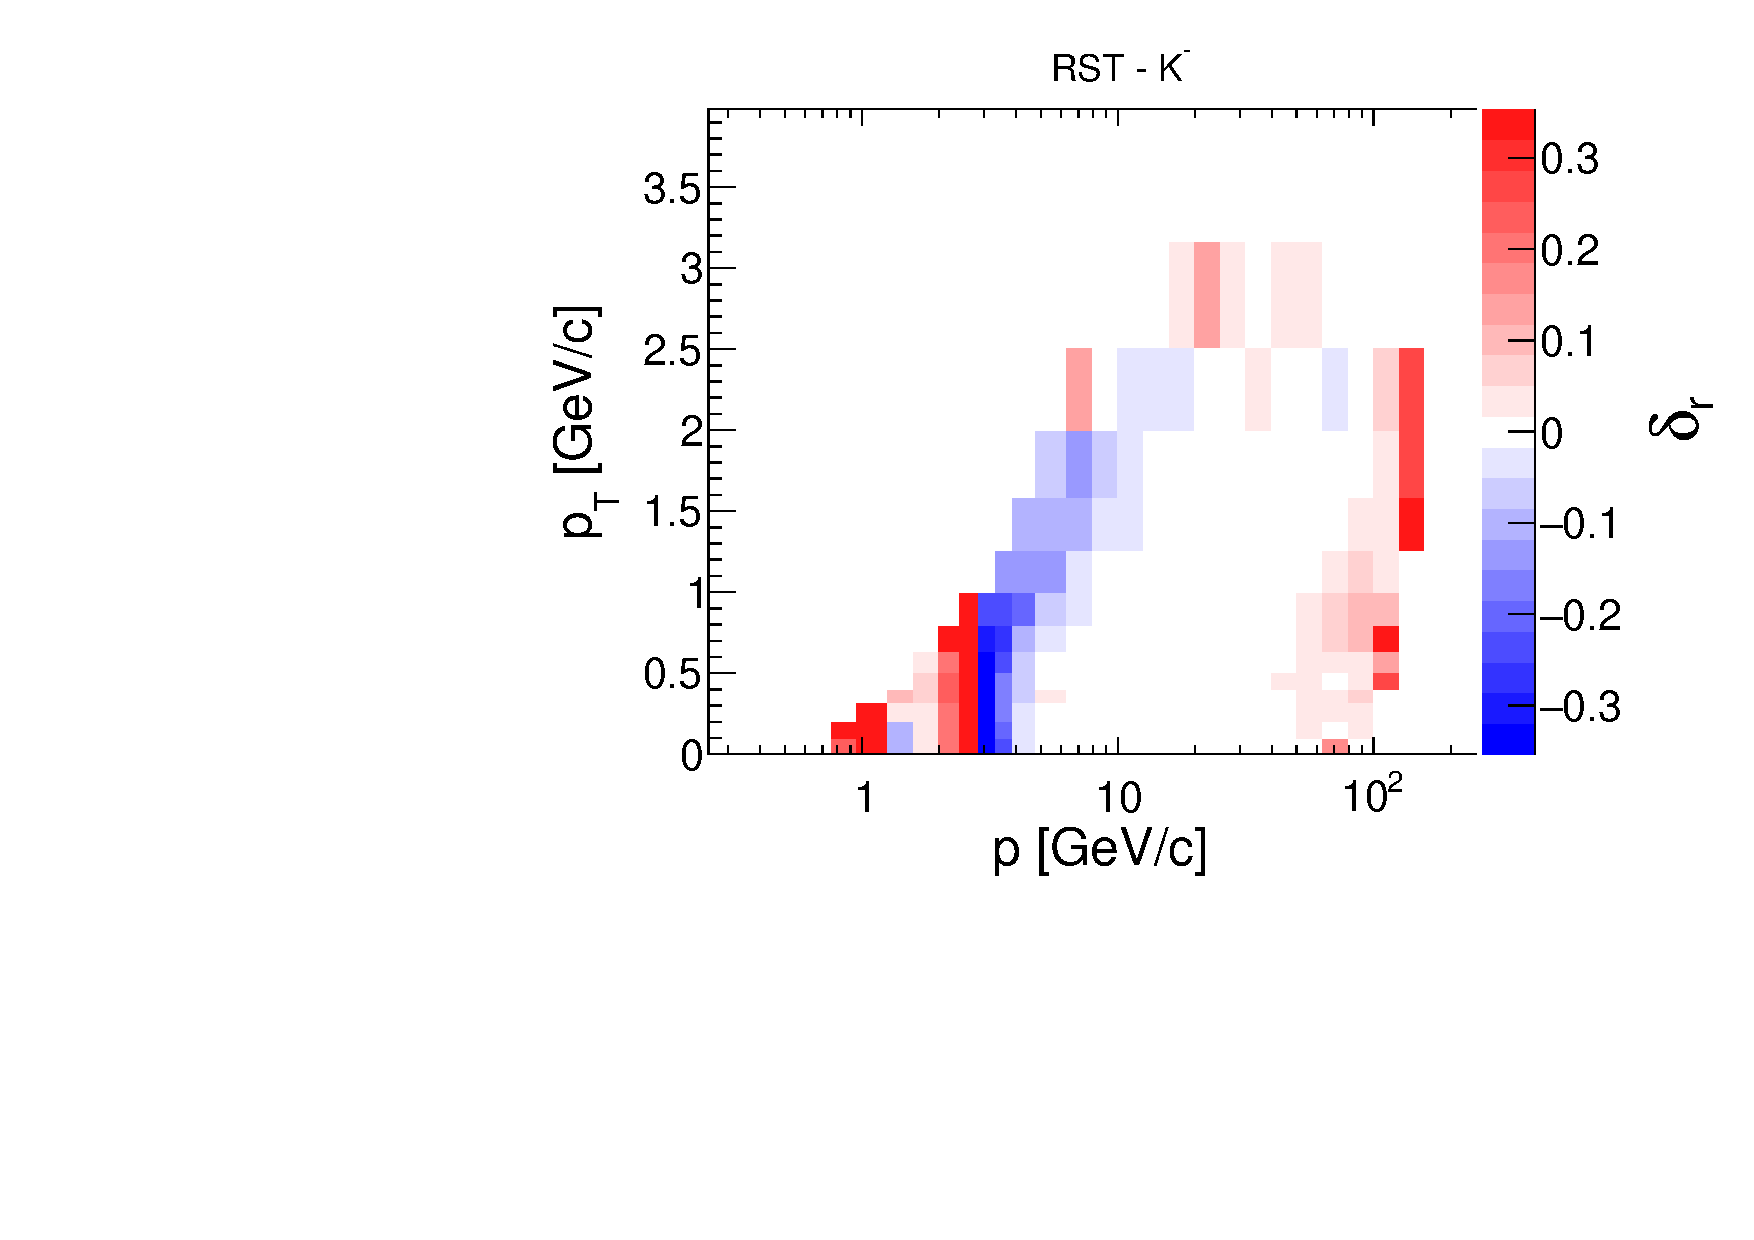
\includegraphics[clip, rviewport=0 0.13 1 0.94,width=0.4\textwidth]{dedx/fake_rel_dev_158_fl0_v0_c0_p2}
  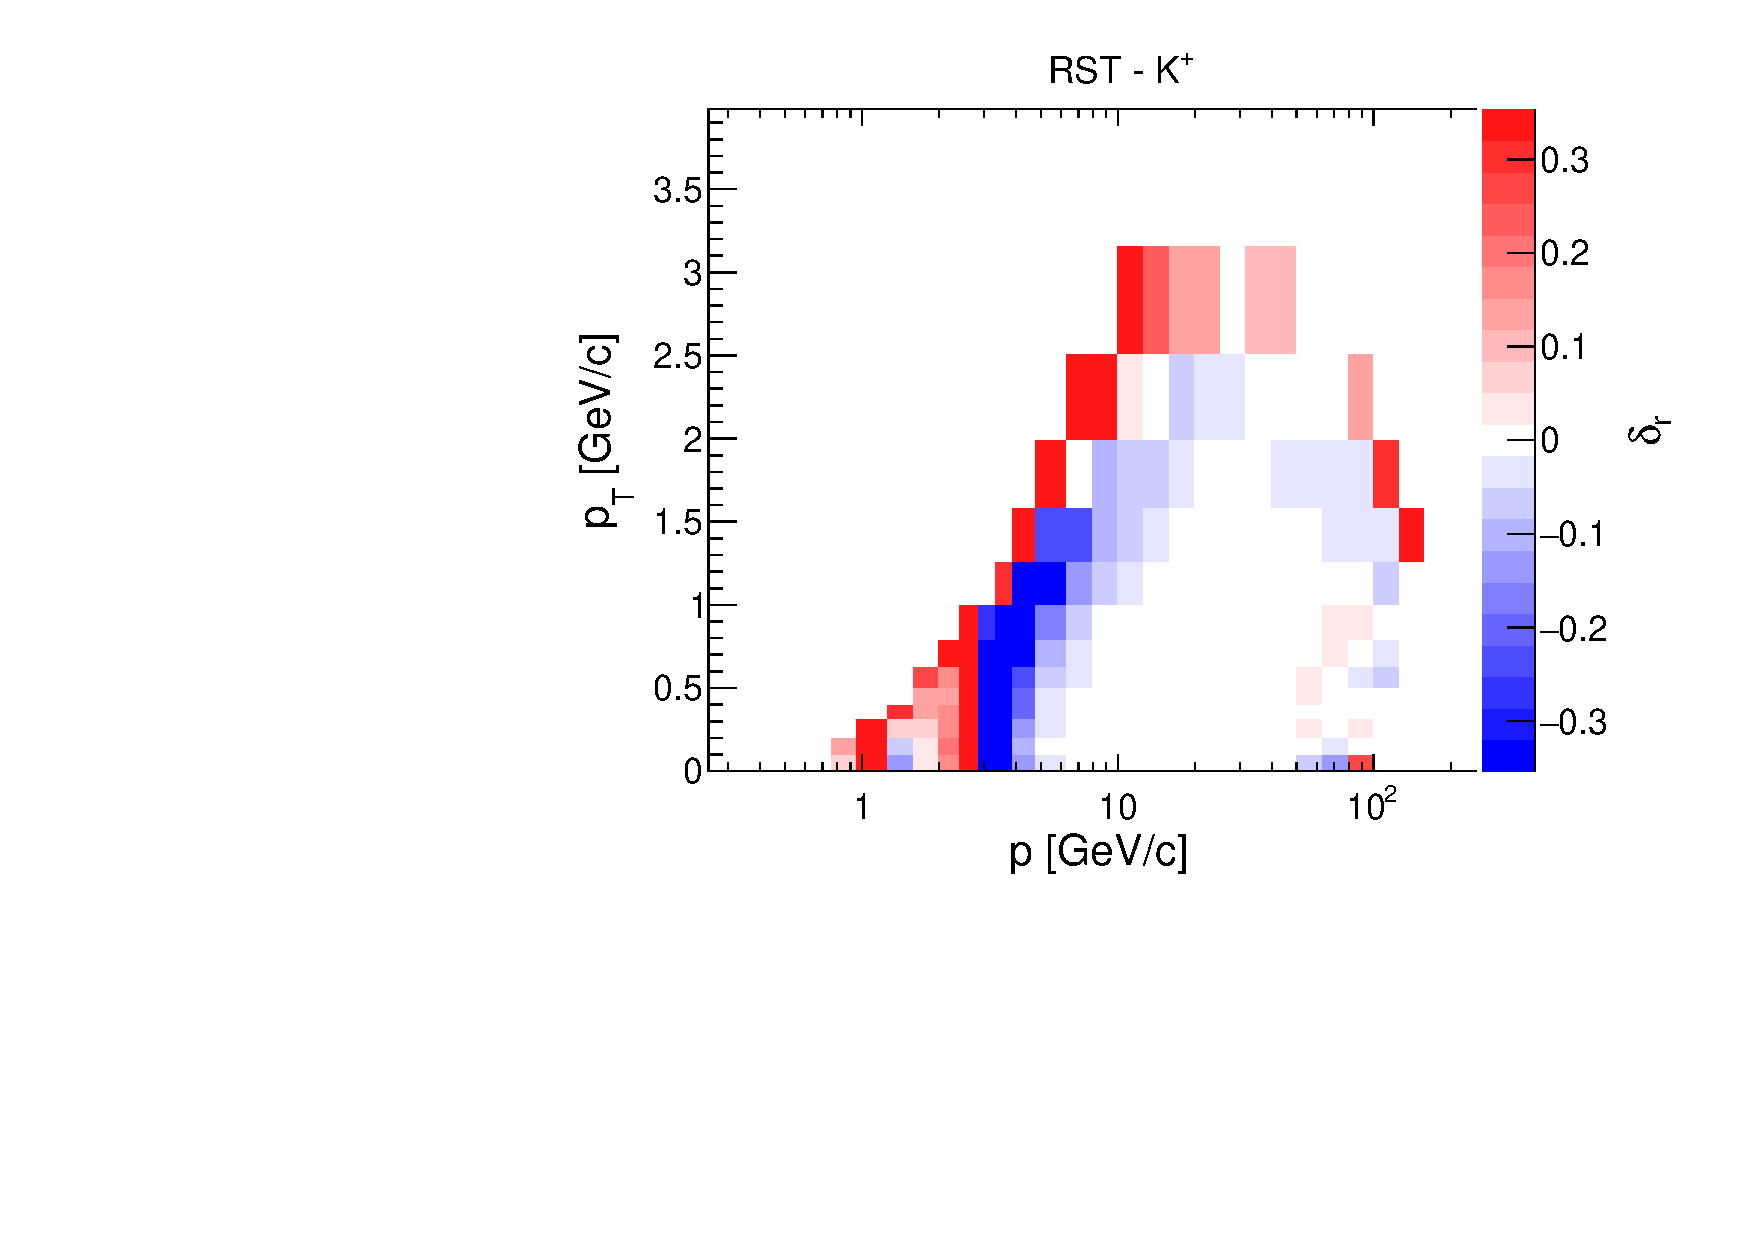
\includegraphics[clip, rviewport=0 0.13 1 0.94,width=0.4\textwidth]{dedx/fake_rel_dev_158_fl0_v0_c1_p2}

  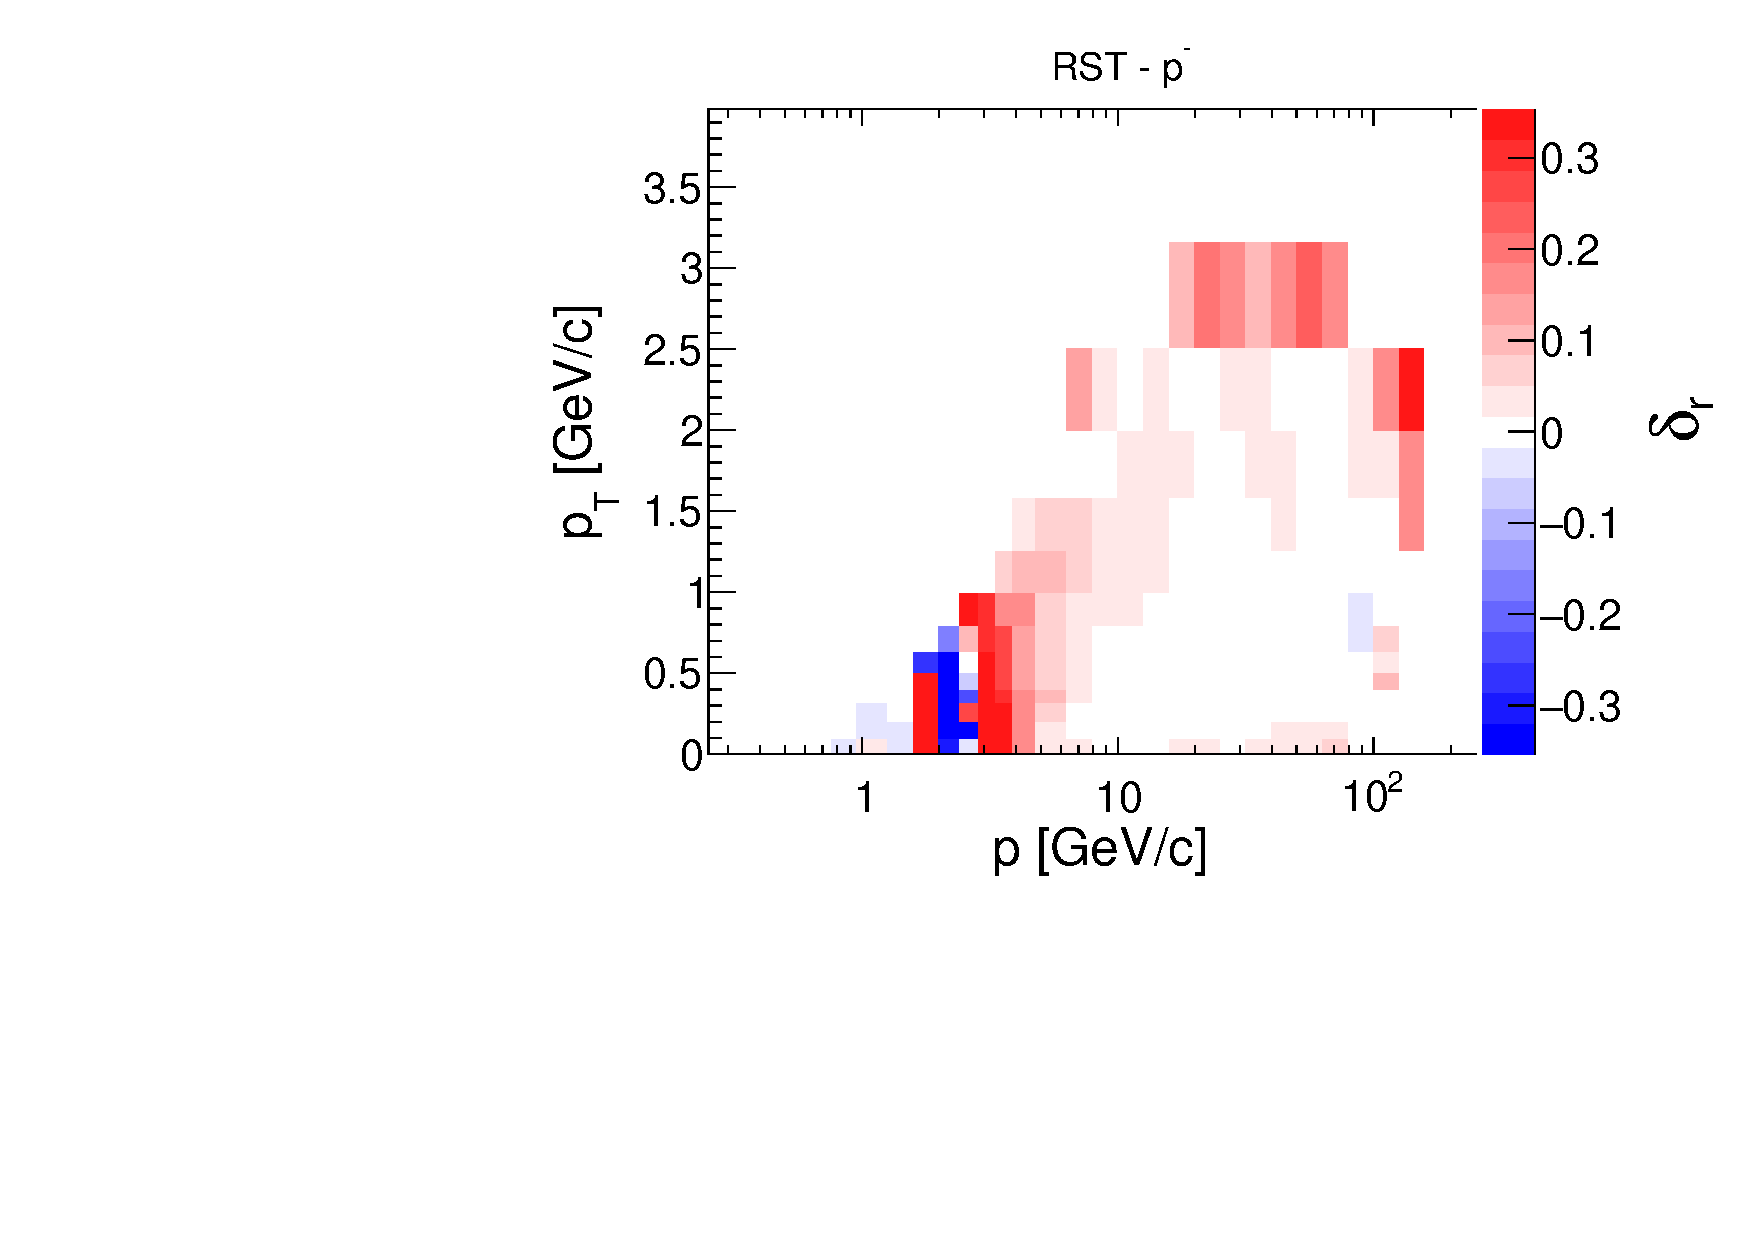
\includegraphics[clip, rviewport=0 0 1 0.94,width=0.4\textwidth]{dedx/fake_rel_dev_158_fl0_v0_c0_p3}
  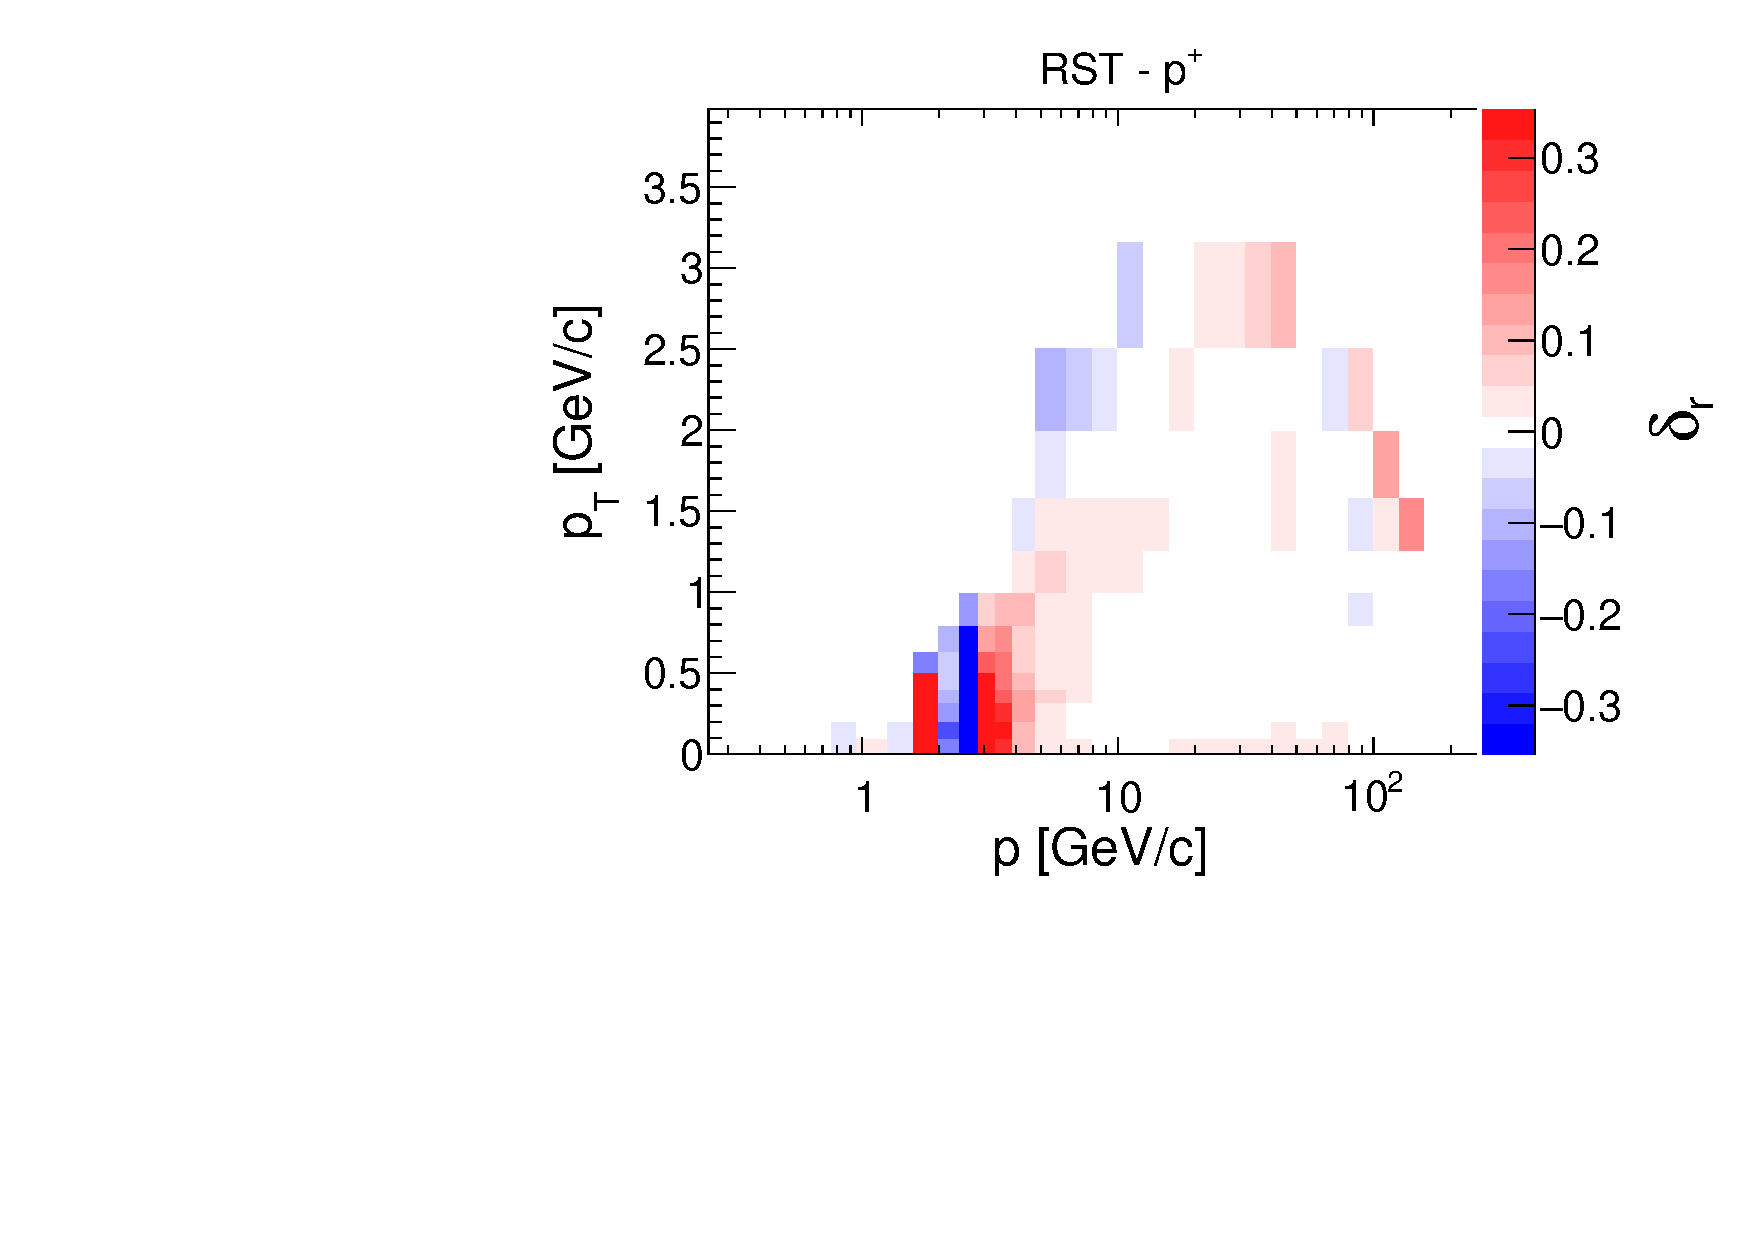
\includegraphics[clip, rviewport=0 0 1 0.94,width=0.4\textwidth]{dedx/fake_rel_dev_158_fl0_v0_c1_p3}


  \caption{Average relative bias of the particle fractions obtained with SDEs for RST and 158 \GeVc dataset.}
  \label{fig:hadron:dedx:fit:fake:reldev158r}
\end{figure}

From the $\sigma_r$ one can clearly see
that for few \pp bins, mainly between 1 and 10 \GeVc,
the fitted fractions present a very large relative
standard deviation in comparison to the remaning phase space regions.
This is because of the proximity between the mean of the
\dedx distribution of two particle types that cause
a partial degeneracy between their fractions. The result
of the \dedx fit at these phase space bins are evidently not
suitable and because of that they will be removed from our analysis.
To this aim, the bins with $\sigma_r$ larger than 0.15 for \pions,
and 0.25 for \kaons and \protons were removed. 

From the $\delta_r$ we can observe that there are regions
of the phase space which presents a significant relative
bias on the fractions.
These regions are mainly the low statistic and the high \pp
bins. In the latter case, the fraction are biased because
the \dedx distributions of all particle types
approach to each other following the relativistic rise
behavior of the deposit energy function.
Attempts were made to eliminate this bias
by changing the fit strategy, however, we found no effective solution.
Therefore, we have decided for a correction procedure based on
the $\delta_r$ obtained from the SDEs.
The multiplicative correction factors is called $c$ and is shown
in~\cref{fig:hadron:dedx:fit:fake:cor158r} for the RST and 158 \GeVc case,
while the remaning cases are shown
in~\cref{fig:hadron:dedx:fit:fake:cor158w,fig:hadron:dedx:fit:fake:cor350r,fig:hadron:dedx:fit:fake:cor350w}.
The phase space bins removed the criteria described above are shown
as white bins.

Besides the cuts and corrections, the SDEs can also
be used to compute the statistical uncertainties of the particle fractions.
This was one by computing the standard deviation of
fractions obtained from the SDEs.


%The fit performance can be studied by means of the
%pull distributions of the particle fractions.
%In~\cref{}

\note{pull distributions?}

\note{discussions here}

%%%%%%%%%% COR %%%%%%%%%%%%%%
\begin{figure}[!ht]
  \centering
  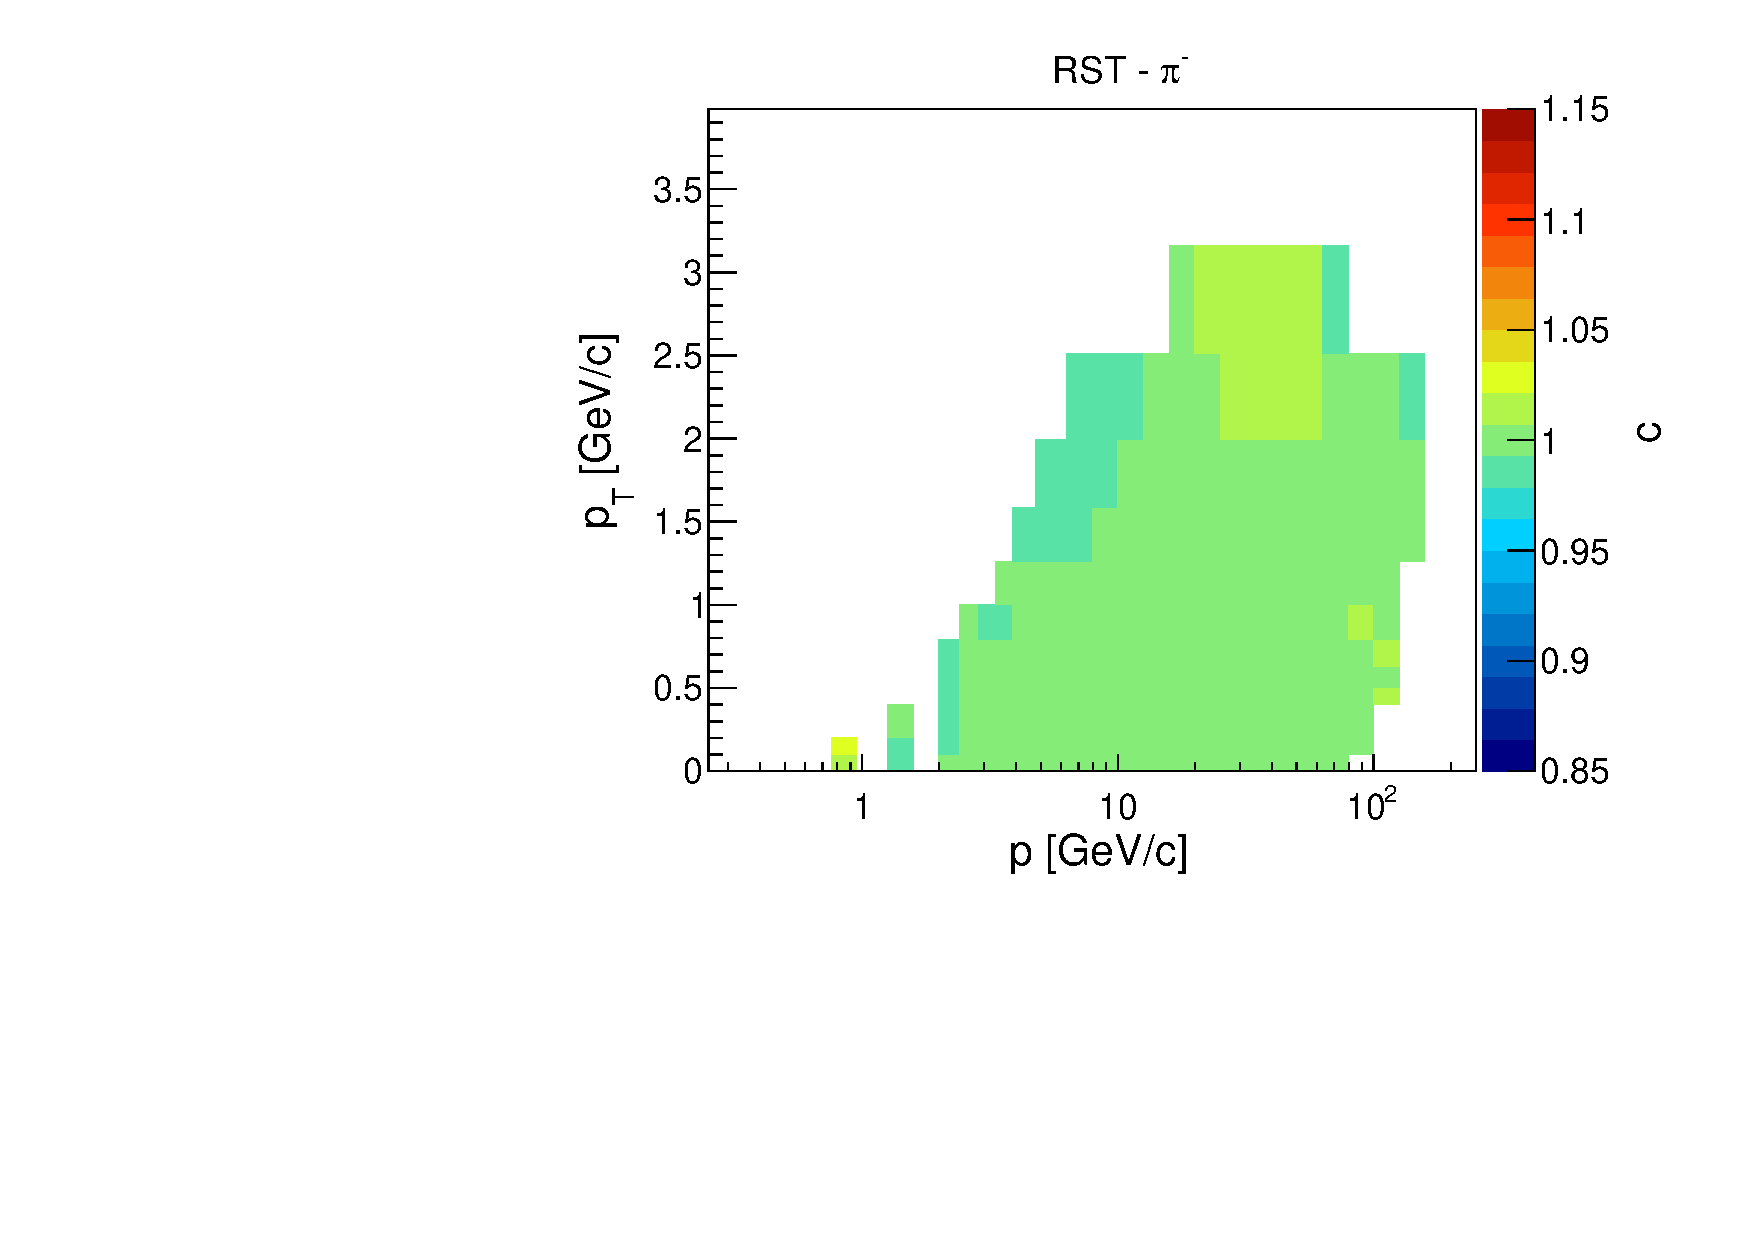
\includegraphics[clip, rviewport=0 0.13 1 0.94,width=0.4\textwidth]{dedx/cor_158_v0_c0_p1}
  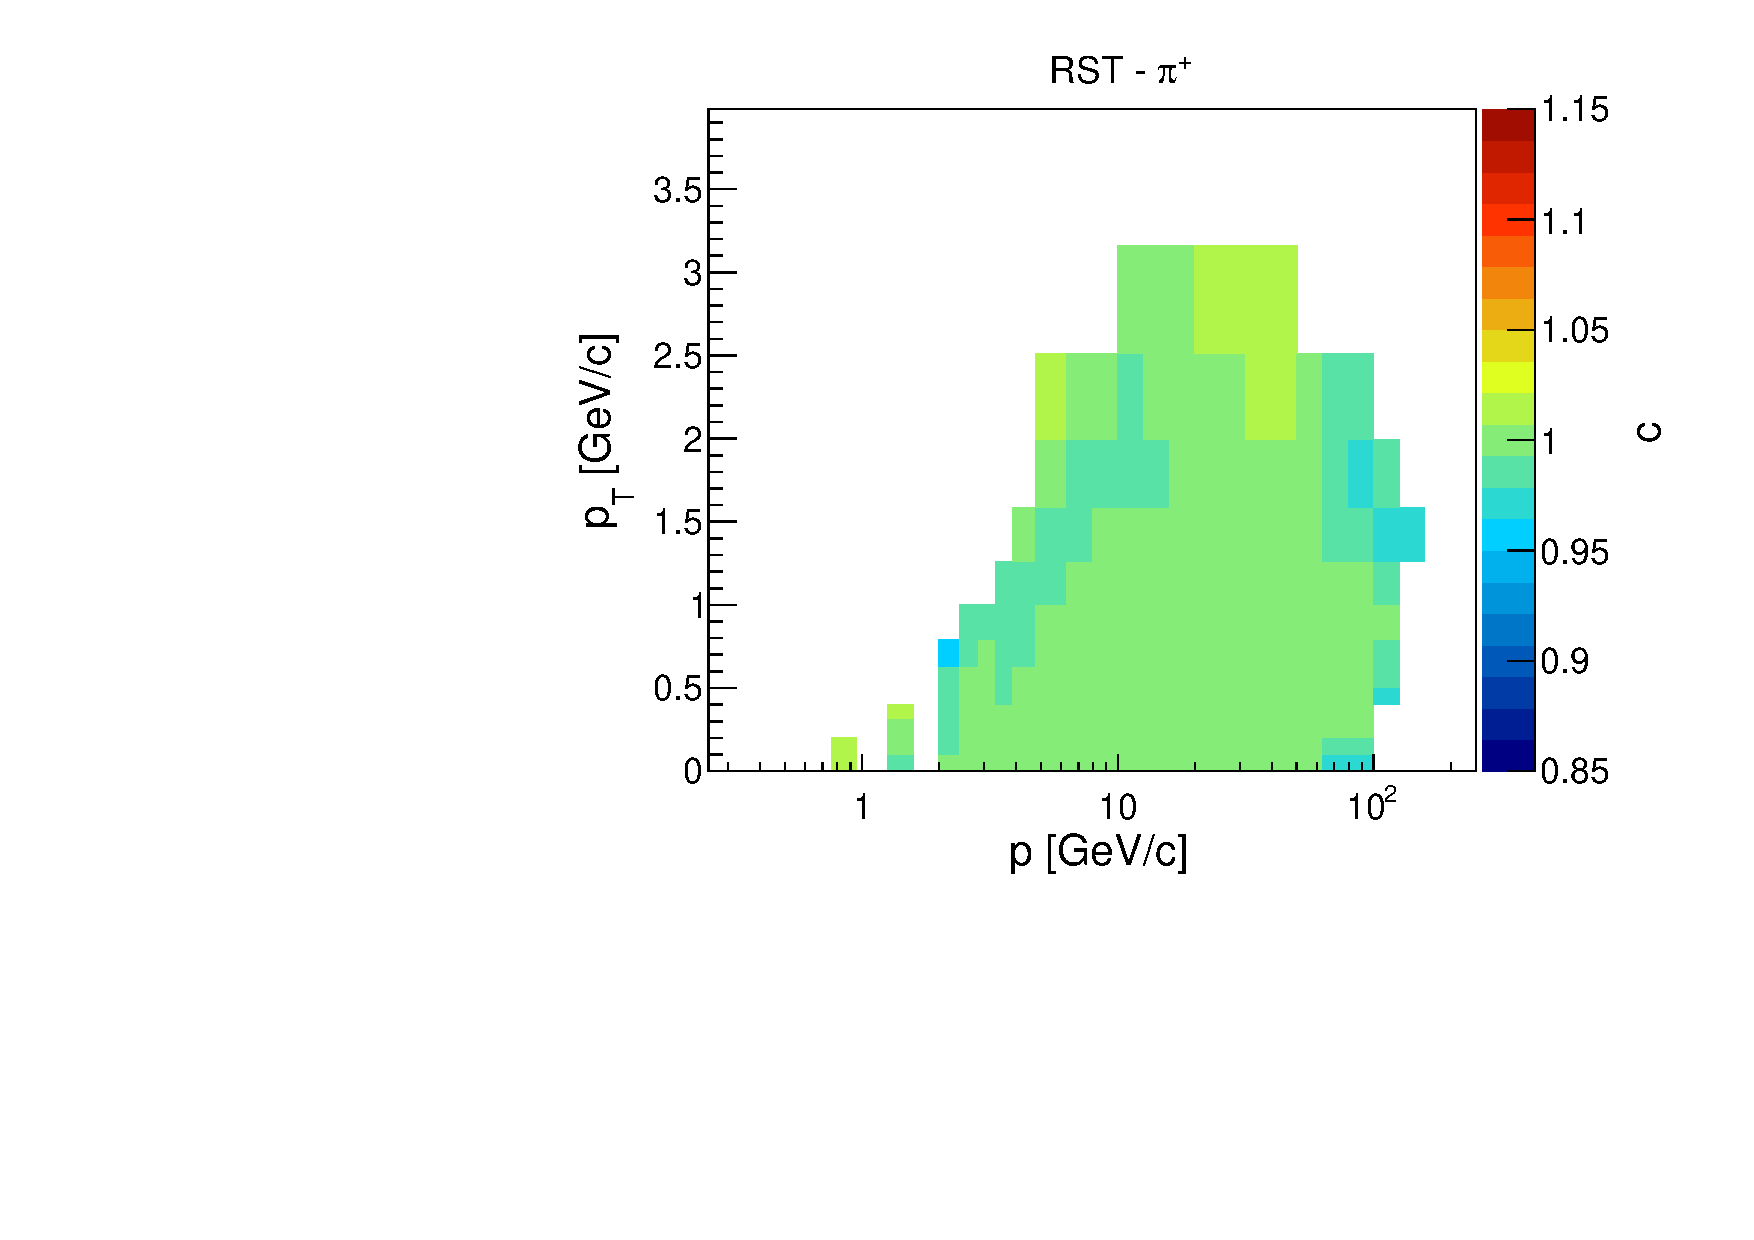
\includegraphics[clip, rviewport=0 0.13 1 0.94,width=0.4\textwidth]{dedx/cor_158_v0_c1_p1}

  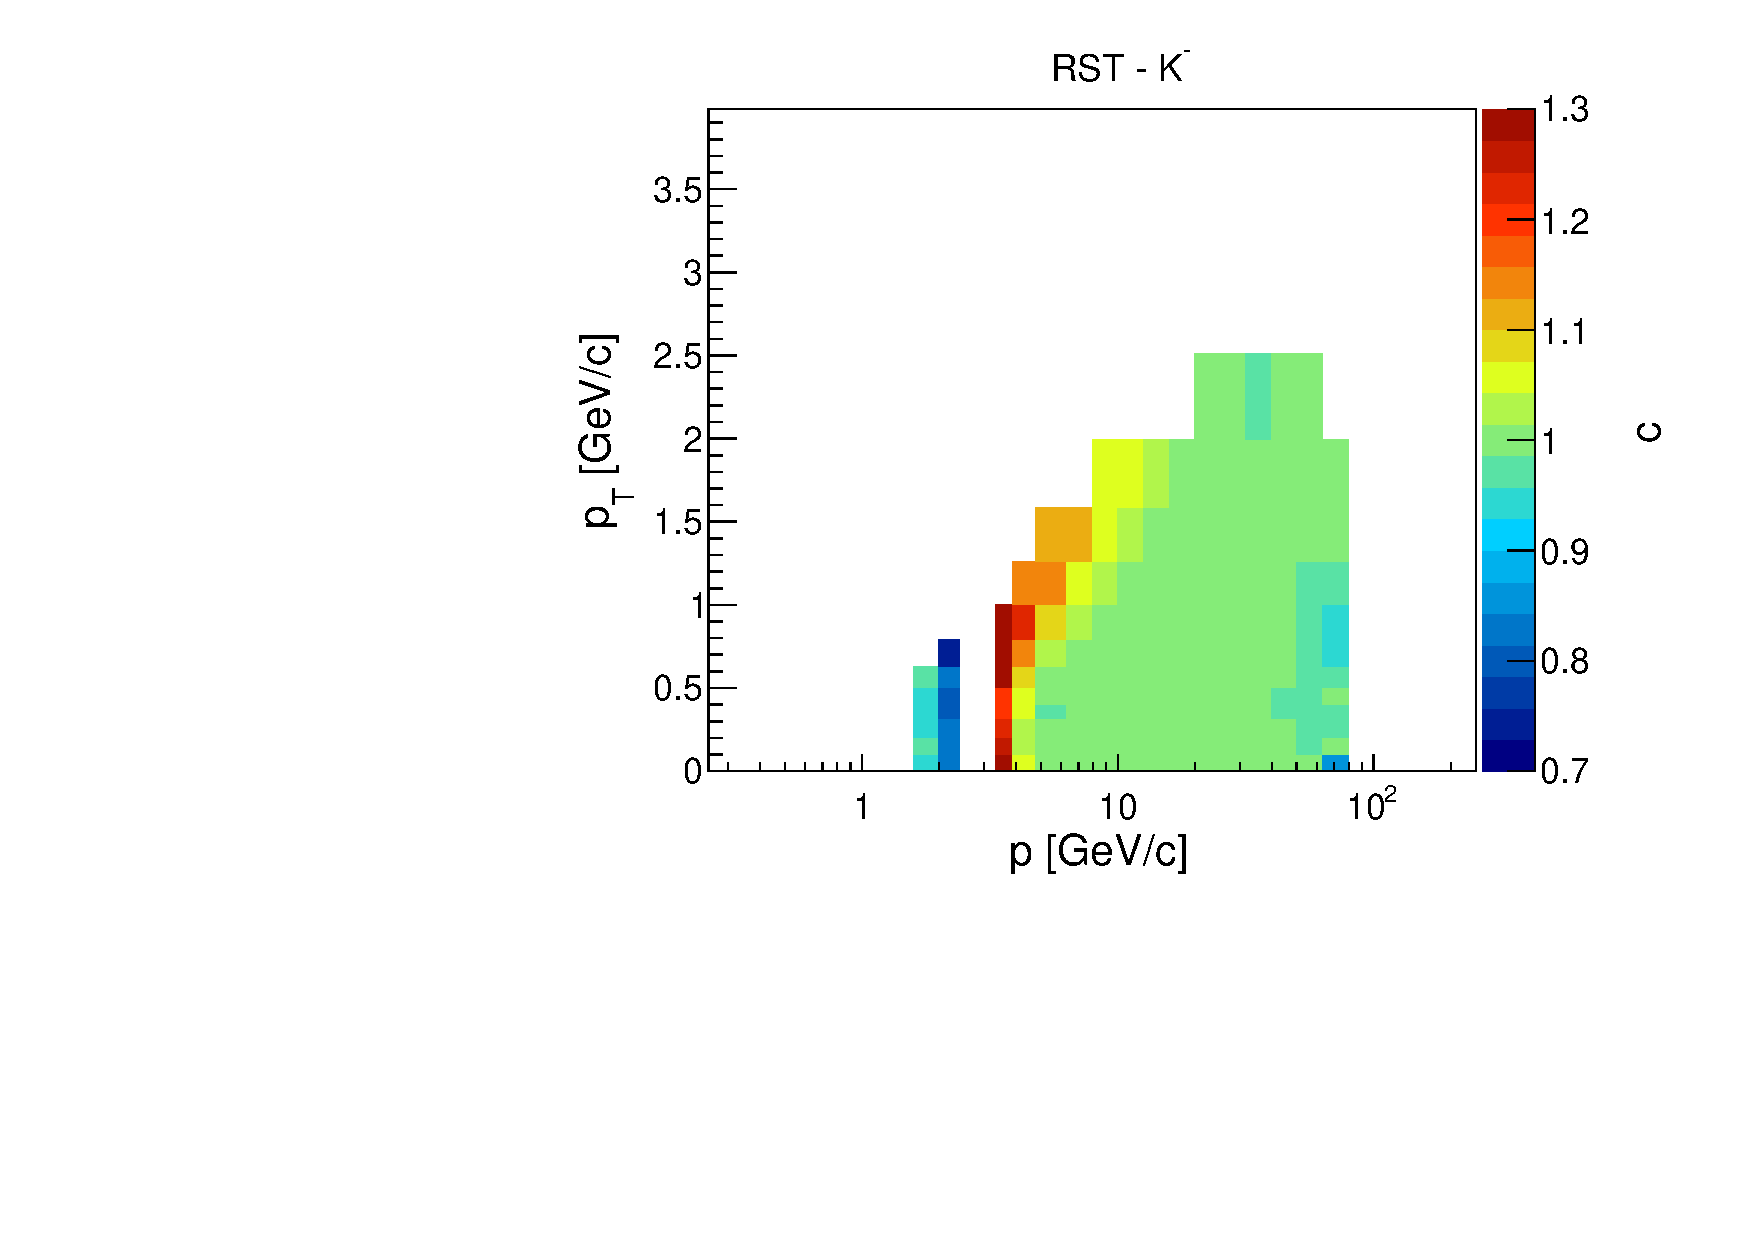
\includegraphics[clip, rviewport=0 0.13 1 0.94,width=0.4\textwidth]{dedx/cor_158_v0_c0_p2}
  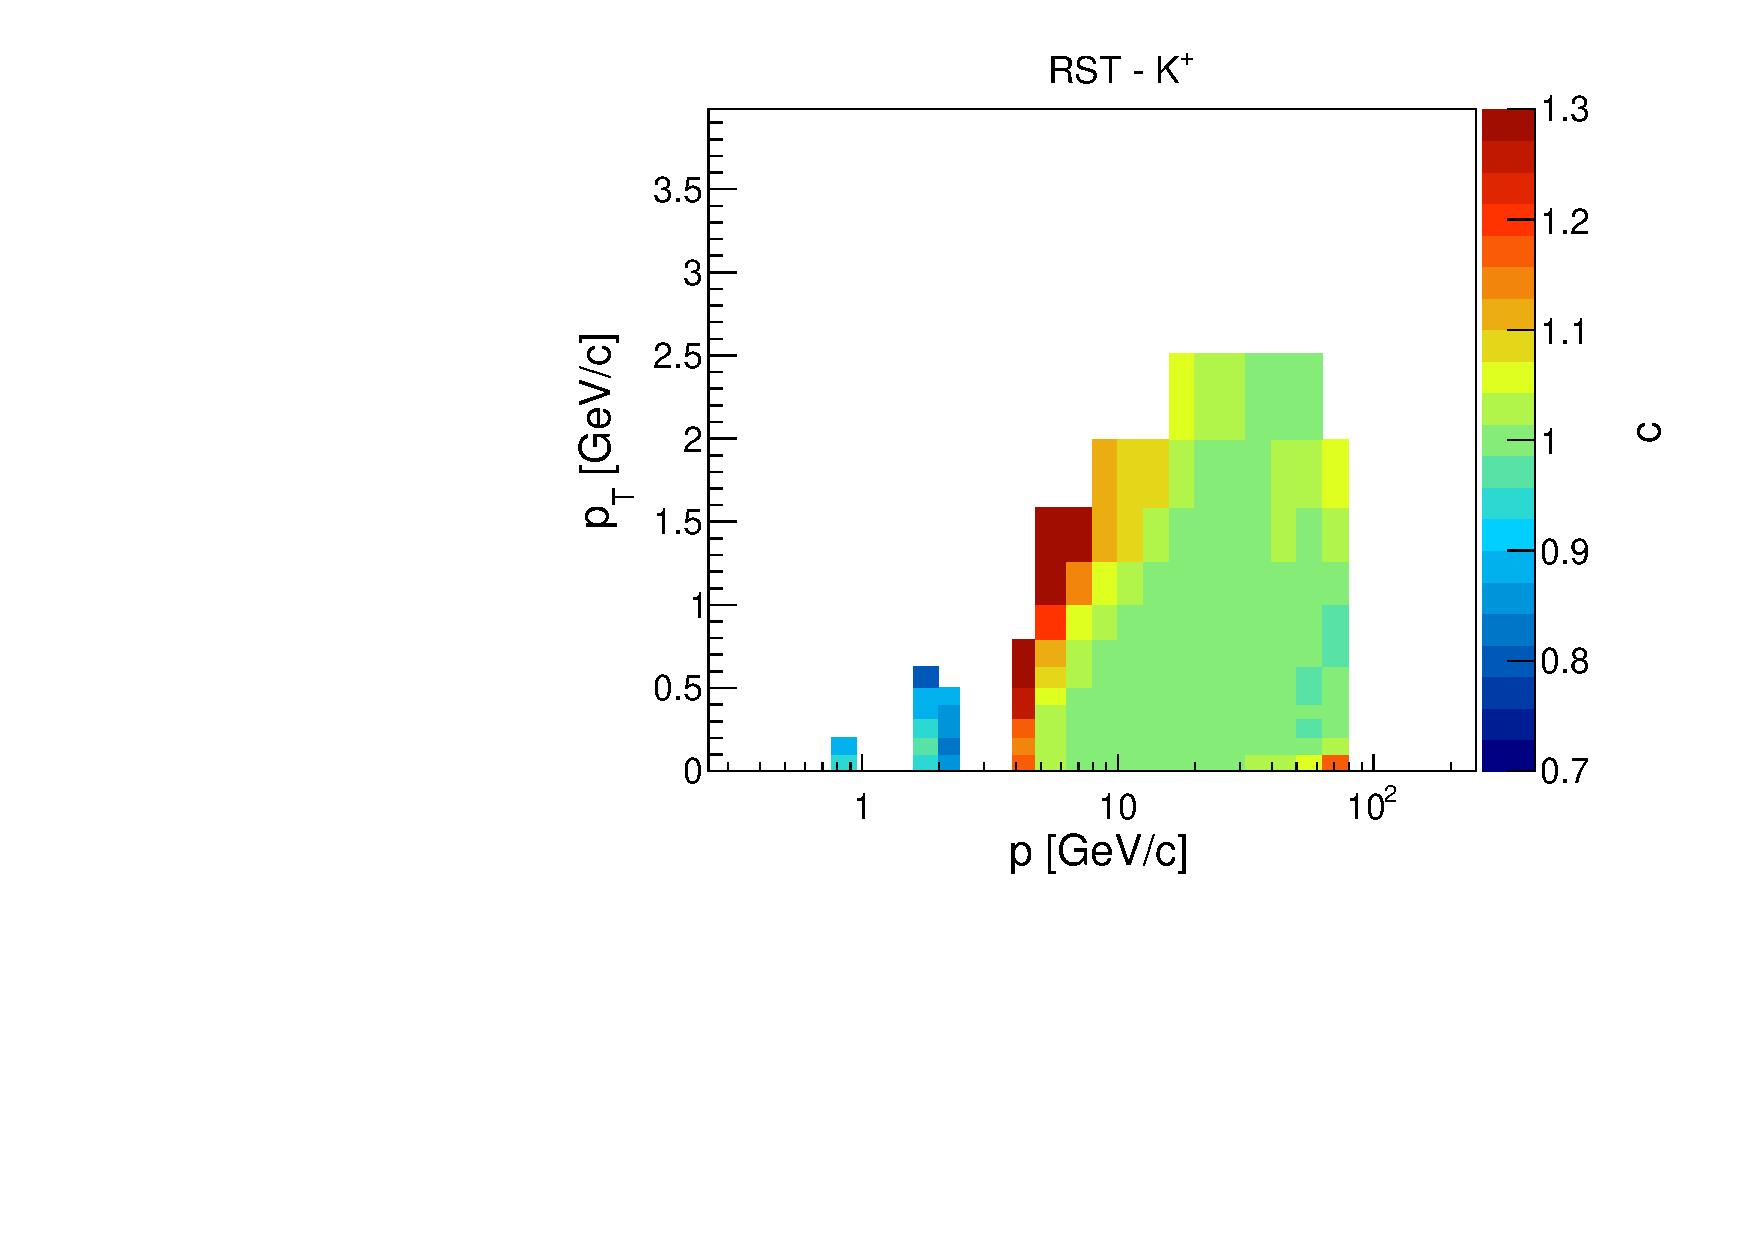
\includegraphics[clip, rviewport=0 0.13 1 0.94,width=0.4\textwidth]{dedx/cor_158_v0_c1_p2}

  \includegraphics[clip, rviewport=0 0 1 0.94,width=0.4\textwidth]{dedx/cor_158_v0_c0_p3}
  \includegraphics[clip, rviewport=0 0 1 0.94,width=0.4\textwidth]{dedx/cor_158_v0_c1_p3}

  \caption{Correction factor for RST and 158 \GeVc dataset.}
  \label{fig:hadron:dedx:fit:fake:cor158r}
\end{figure}


%%%---------------------------------%%%%
\subsection{Particle identification results}
\label{sec:hadron:dedx:results}

After applying the cuts and corrections discussed
in~\cref{sec:hadron:dedx:sde} we obtain the final
particle fractions to be used to compute the spectra.
In~\cref{fig:hadron:dedx:fit:final158r} we show examples
of the final fractions for RST and 158 \GeVc dataset,
while the remaning cases are shown 
in~\cref{fig:hadron:dedx:fit:final158w,fig:hadron:dedx:fit:final350r,fig:hadron:dedx:fit:final350w}.
Only the three particle types of interested are shown: $\pi$, $K$ and $p$.
Each plot shows the fractions as a function of \pp for one \pT bin.
The equivalent plots for the target removed dataset are shown
in~\cref{fig:hadron:dedx:fit:out158r,fig:hadron:dedx:fit:out158w,fig:hadron:dedx:fit:out350r,fig:hadron:dedx:fit:out350w}.

%%%%%%%%%% FRACTION %%%%%%%%%%%%%%
\begin{figure}
  \centering
  \includegraphics[clip, rviewport=0 0 1 1,width=1.00\textwidth]{dedx/fraction_pt_158_fl2_v0}
  \caption{Particle fractions obtained from the \dedx fit of the RST and 158 \GeVc dataset, with target inserted.}
  \label{fig:hadron:dedx:fit:final158r}
\end{figure}


%%%%%%%%%%%%%%%%%%%%%%%%%%%%%%%%%%%%%%%%
\section{\vzero analysis}
\label{sec:hadron:vzero}


%%%---------------------------------%%%%
\subsection{Signal extraction}
\label{sec:hadron:vzero:signal}


\subsubsection{\vzero cuts}
\label{sec:hadron:vzero:signal:cuts}


%%%%%%%%%%%%%%%%%%%%%%%%%%%%%%%%%%%%%%%%
\section{Monte Carlo corrections}
\label{sec:hadron:correction}


The measured number of events, tracks and \vzeros
particles in a given phase space bin are naturally biased by
detector effects. To determine the final spectra,
these effects must be corrected, and that
is done by applying a correction factor obtained
from Monte Carlo simulations. This factor is called here \cmc.
For a given phase space bin, \cmc is basically the ratio
between the generated and measured spectra and it
is written as
\begin{equation}
  \cmc = \left( \frac{n^\gen}{N^\gen} \right) / \left( \frac{n^\sel}{N^\sel} \right).
  \label{eq:hadron:correction:cmc}
\end{equation}
where $N$ refers to number of events and $n$ can be either the number of
tracks, for the identified spectra analysis, or the number
of \vzeros, for the \vzero analysis.
The indexes \gen and \sel refer to generated and selected quantities and,
while the first is obtained directly from the Monte Carlo generators,
the second is obtained by the detector simulations, in which the
reconstruction algorithm and selection are exactly the same
as the one applied to data.
For the sake of clearness, the \cmc can be split in the
event and track or \vzero contributions, which will be refereed as
$\alpha$ and $\beta$. In this way, \cmc becomes
\begin{equation}
  \cmc = \left( \frac{N^\sel}{N^\gen} \right) / \left( \frac{n^\sel}{n^\gen} \right) = \alpha / \beta.
  \label{eq:hadron:correction:cmc:2}
\end{equation}
The $\alpha$ factor is common to all the datasets,
while the $\beta$ is different for each phase space bin. 

The \cmc was determined here by 
the three simulation sets, generated with different hadronic
interaction models (see~\cref{sec:hadron:data}).
The $\alpha$ factor obtained is summarized
in~\cref{tab:hadron:alpha}, where we show the values for each simulation
set and their average value, which will be used in this work. 
The observed differences in the $\alpha$ factor due
to the hadronic interaction models are expected mainly
because of the large discrepancy between the particle
multiplicities. As an illustration, we can take the \DPMJetLong
case, in which the average multiplicity is
fairly larger than the others and consequently the
$\alpha$ is also significantly larger. 
This relation is caused mainly by two effects. First,
the interaction trigger probability is larger on average
because the larger number of particles crossing the detector.
Second, the cut on the Z position of the main vertex
tends to remove less events since, with more detected particles,
the fit of main vertex tends to be more precise.
The model dependence of the $\alpha$ will be accounted
on the systematic uncertainties in~\cref{sec:hadron:spec:syst}.

\begin{table}
  \begin{center}
    \begin{tabular}{|r|c|c|} \hline
      & 158 GeV/c & 350 GeV/c \\ \hline
      \EposLong   & 0.875     & 0.744 \\
      \DPMJetLong & 0.949     & 0.848 \\
      \QGSJetLong & 0.868     & 0.721 \\ \hline
      Average     & 0.897     & 0.771 \\ \hline
    \end{tabular}
    \caption{}
    \label{tab:hadron:alpha}
  \end{center}
\end{table}

The $\beta$ factor for \pions, \kaons and \protons
is computed by the ratio of the generated and
measured number of tracks. 
In~\cref{fig:hadron:correction:beta:dedx158,fig:hadron:correction:beta:dedx350}
we show the $\beta$ for these particles.
For the \vzero particles, \lambs and \kzeros, the $\beta$
is computed as the ratio between the \vzero particles generated and
measured in a given phase space bin.
In~\cref{fig:hadron:correction:beta:vzero158,fig:hadron:correction:beta:vzero350}
we show the $\beta$ for these particles.
It is important to note that the $\beta$ factor
for the \vzero particle includes the effect
of the \vzero cuts, presented in~\cref{sec:hadron:signal:cuts}.


%%%%%%%%%% BETA %%%%%%%%%%%%%%%%
\begin{figure}
  \centering
  \includegraphics[clip, rviewport=0 0.13 1 0.94,width=0.4\textwidth]{dedx/fac_158_All_beta_c0_p1}
  \includegraphics[clip, rviewport=0 0.13 1 0.94,width=0.4\textwidth]{dedx/fac_158_All_beta_c1_p1}

  \includegraphics[clip, rviewport=0 0.13 1 0.94,width=0.4\textwidth]{dedx/fac_158_All_beta_c0_p2}
  \includegraphics[clip, rviewport=0 0.13 1 0.94,width=0.4\textwidth]{dedx/fac_158_All_beta_c1_p2}

  \includegraphics[clip, rviewport=0 0.13 1 0.94,width=0.4\textwidth]{dedx/fac_158_All_beta_c0_p3}
  \includegraphics[clip, rviewport=0 0.13 1 0.94,width=0.4\textwidth]{dedx/fac_158_All_beta_c1_p3}

  \caption{$\beta$ correction factor for the 158 \GeVc dataset.}
  \label{fig:hadron:correction:beta:dedx158}
\end{figure}

%%%%%%%%%%% BETA %%%%%%%%%%%%%%%%%%
\begin{figure}
  \centering
  \includegraphics[clip, rviewport=0 0 1 1,width=0.95\textwidth]{vzero/beta158}
  
  \caption{$\beta$ correction factor for the 158 \GeVc dataset.}
  \label{fig:hadron:correction:beta:vzero158}
\end{figure}

The geometrical acceptance of the detector
is the dominant contribution to the $\beta$ factor
for both identified spectra and \vzero cases.
Smaller effects, but still significant, are related
to the event selection, track reconstruction efficiency, 
bin migration and feed-down from re-interactions and weak decays.
Apart from the feed-down from weak decays,
the model dependence due to all these effects is very small.
In particular the model dependence of the event selection
contribution can reach few percents. This differences
will be taken into account in the systematic uncertainty estimation.
See~\cref{sec:hadron:spec:syst} for more details.
On the other hand, the feed-down contribution from weak decays
is the only one that can present a large model
dependence, reaching up to YYY\%.  
Given that the feed-down contribution itself
can reach up to 20\% of the total $\beta$
correction, we must give it more attention.


Concerning the charged particles, \pions and \protons
are strongly fed by the decay of \lambs and \kzeros,
with a small contribution from other particles.
In~\cref{} we show all the particles that decay in
\pions, \kaons and \protons within their relative abudance(?),
obtained with the model \EposLong.
The \kaons in turn are weakly fed only by YYY, and YYY.
Since the \lambs and \kzeros production is very different
among the hadronic interaction models, the model dependence
on the $\beta$ correction for \pions and \protons would
naturally be very large. To avoid that, in this work the
measured spectra of \lambs and \kzeros will be used
to correct the feed-down contribution from these particles.
The description of the procedure adopted by us is given
in~\cref{sec:hadron:correction:fd}.


Concerning the \lambs and \kzeros,
the particles that contribute to the feed-down
are shown in~\cref{} for the hadronic model \EposLong.
In this case the model differences are still
large and they will be accounted for in the systematic
uncertainties (see~\cref{sec:hadron:spec:syst}). 



%%%---------------------------------%%%%
\subsection{Feed-down}
\label{sec:hadron:correction:fd}




%%%%%%%%%%%%%%%%%%%%%%%%%%%%%%%%%%%%%%%%
\section{Spectra}
\label{sec:hadron:spec}


%%%---------------------------------%%%%
\subsection{Statistical uncertainties}
\label{sec:hadron:spec:stat}


%%%---------------------------------%%%%
\subsection{Systematic uncertainties}
\label{sec:hadron:spec:syst}



%%%%%%%%%%%%%%%%%%%%%%%%%%%%%%%%%%%%%%%%
\section{Results}

%%%%%%%%%%%%%%%%%%%%%%%%%%%%%%%%%%%%%%%%
\section{Summary and conclusions}

